\let\orilabel\label
\documentclass[showkeys,noshowpacs,superscriptaddress,pre,preprint]{revtex4-1}
\let\label\orilabel
\usepackage{graphicx}
\usepackage{subcaption}
\usepackage{amsmath}
\usepackage{amssymb}
\usepackage{tikz}
\usetikzlibrary{calc,decorations.markings}
\usepackage[hypertexnames=false]{hyperref}

% REVTeX centers short captions via \hfil...\hfil; use flush-left (APS/PRE convention).
\makeatletter
\long\def\@makecaption#1#2{%
  \par
  \vskip\abovecaptionskip
  \begingroup
   \small\rmfamily
   \flushing
   \let\footnote\@footnotemark@gobble
   \@make@capt@title{#1}{#2}\par
  \endgroup
  \vskip\belowcaptionskip
}
\makeatother
\captionsetup{justification=raggedright,singlelinecheck=false,skip=0.5em}

% Submission figure numbering (independent of float counter increments per page).
\newcounter{submitfig}
\newcounter{submitpanel}
\renewcommand{\thesubmitfig}{\arabic{submitfig}}
\renewcommand{\thesubmitpanel}{\arabic{submitfig}(\alph{submitpanel})}

% Panel tag only — visual label without REVTeX auto-caption text.
\newcommand{\figurepaneltag}[1]{%
  \par\medskip
  {\centering\small\rmfamily #1\par}%
}

% Standalone submission figure (one number, one page).
\newcommand{\registerstandalonefigurelabel}[1]{%
  \refstepcounter{submitfig}%
  \phantomsection
  \label{#1}%
}

% Composite figure panel: one number shared; panels become 3(a), 3(b), ...
\newcommand{\registerpanelfigurelabel}[2][]{%
  \ifx\relax#1\relax
    \refstepcounter{submitpanel}%
    \phantomsection
    \label{#2}%
  \else
    \refstepcounter{submitfig}%
    \setcounter{submitpanel}{0}%
    \phantomsection
    \label{#1}%
    \refstepcounter{submitpanel}%
    \phantomsection
    \label{#2}%
  \fi
}

% Legacy name kept for Fig.~1--2; routes to standalone registration.
\newcommand{\registerfigurelabels}[1]{%
  \registerstandalonefigurelabel{#1}%
}

% Traditional submission layout: one panel per page, full text width.
% Optional first argument: composite cross-reference label (e.g., fig:bare-lindhard).
\newcommand{\panelpagefigure}[3][]{%
  \clearpage
  \begin{figure}[p]
    \centering
    \vfill
    \includegraphics[width=\textwidth]{#2}%
    \vfill
    \registerpanelfigurelabel[#1]{#3}%
    \figurepaneltag{Fig.~\thesubmitpanel}%
  \end{figure}%
}

% AFOSR grant number: replace placeholder when award ID is confirmed.
\newcommand{\afosrgrantnumber}{FA9550-XX-XXXX}

\begin{document}
\title{Linear response representation of two-fermion plasmas}
\author{In-Gee Kim}
\email{kim.ingee@bonasapiens.com}
\affiliation{Bona Sapiens, Inc., Seoul 07332, Republic of Korea}

% \author{Michael S. Murillo}
% \email{murillom@msu.edu}
% \affiliation{Department of Computational Mathematics, Science and Engineering and Department of Chemical Engineering and Materials Science, Michigan State University, East Lansing, Michigan 48824, USA}

\date{\today}

\begin{abstract}
We present a deterministic, causality-constrained formulation for the finite-temperature Lindhard linear response and two-component random-phase approximation (RPA) dielectric functions, resolving analytic inconsistencies in widely used routes based on contour integration over Matsubara frequencies. We demonstrate that pole-summation formulations---which assemble the real susceptibility from infinite residue sums over Matsubara-like poles---fail through violations of Jordan's lemma, divergent series tails, and order interchanges not justified by Fubini's theorem; hybrid treatments that combine grand-canonical dissipation with canonical contour sums further induce ensemble inconsistency, breaking exact causality and producing persistent $\mathcal{O}(1)$ real-part offsets from exact $T=0$ analytical limits in the highly degenerate regime. Elevating the Kramers--Kr\"onig relation to the primary construction principle rather than an \emph{a posteriori} consistency check, we derive the imaginary part in closed form within the grand-canonical ensemble and obtain the real part solely as its Hilbert transform on a strictly constrained real-axis physical space, bypassing the infinite Matsubara pole barrier entirely. By employing a modified sinc-quadrature rule with theoretical truncation error bound $\mathcal{O}(\sqrt{N} \exp(-\sqrt{\pi d \alpha N}))$ (where $N$ is the truncation limit, $d$ is the half-width of the analytic strip, and $\alpha$ is a convergence parameter), we achieve evaluation accuracy exponentially suppressed well below machine precision ($\sim 10^{-259}$ for $N=16384$, $d/\alpha=7$). We validate this deterministic framework by extracting the electron plasmon dispersion and exact Landau damping via derivative-free root finding, and by demonstrating precise satisfaction of four macroscopic dynamic structure factor sum rules within machine precision without ad hoc regularization or parameter tuning.
\end{abstract}
%\pacs{52.25.Mq, 52.27.Cm, 05.30.Fk, 71.45.Gm}
\keywords{Plasma physics; Multicomponent plasmas; Electron gas; Dielectric function; Dynamic structure factor; Random phase approximation; Linear response; Kramers--Kr\"onig relations}
\maketitle

\section{Classical representation}
\label{sec:classical}

A classical system is specified by the classical potential $u(q)$, 
where $q = \left| \mathbf{q} \right|$ is the length of the reciprocal vector for the homogeneous and isotropic system.
The classical potential is determined by a requirement that 
the corresponding structure factor $S (q)$ is the same as the realistic quantum structure factors $S_Q(q)$, 
which are supposed to be known from quantum mechanics,
of the homogeneous and isotropic plasma with density $n$.

From the classical linear response theory~\cite{Ichimaru1973},
the static structure factor of a monatomic gas at a given temperature $T$ is given by
\begin{equation}
{S(q)} = {\chi_0}^{-1} {\chi (q)},
\label{classical-structure-factor}
\end{equation}
where $\chi_0 = - n/k_\mathrm{B} T$ is the classical ideal gas density response 
and ${\chi (q)}$ is the classical susceptibility.
When we introduce a potential $u(q)$ describing the interparticle interaction, 
the structure factor form may be corrected,  
in spirit of the random phase approximation (RPA), 
to include the effects of this interaction
\begin{equation}
{S(q)} = {\chi_0}^{-1} \frac{\chi_0}{1 - {u(q)} \chi_0} .
\label{classical-rpa}
\end{equation}
This implies that one can always possible 
to find the classical interaction potential ${u(q)}$ of a gas with the density $n$ and temperature $T$
if one is well informed about the structure factor ${S(q)}$.
The explicit procedure for this inversion is as follows: 
\begin{eqnarray}
\left( 1 - {u(q)} \chi_0 \right) {S(q)} &=& 1, \nonumber\\
{u(q)} &=& \frac{1- {S(q)}}{\chi_0 S(q) } \nonumber\\
&=& \left( {\chi_0} {S(q)} \right)^{-1} - {\chi_0}^{-1} .
\label{classical-potential}
\end{eqnarray}
Substituting Eq. (\ref{classical-structure-factor}) into Eq. (\ref{classical-potential}), we get
\begin{equation}
{u(q)} = \chi^{-1} (q) - {\chi_0}^{-1}.
\end{equation}
Therefore, a classical interparticle potential is interpreted as a measure of response deviation of the interacting gas from that of the corresponding ideal gas.
Note that the potential ${u(q)}$ and the responses ${\chi_0}^{-1}$ and ${\chi}^{-1} (q)$ depend 
on the density $n$ and the temperature $T$ implicitly.

Eq. (\ref{classical-rpa}) is quite useful because it does not restrict the information source of ${S(q)}$; 
we can provide ${S(q)}$ either from an experiment or from a quantum mechanical calculation.
For example, ${S(q)}$ may be obtained quantum mechanically~\cite{Giuliani-Vignale2005}, 
for a homogeneous and isotropic gas of $N$ fermions, from the relation
\begin{equation}
{S_\mathrm{Q} (q)} = \frac{1}{N} \int_{- \infty}^{\infty} {d\omega}\, {S_\mathrm{Q} (q, \omega)},
\label{static-structure-factor}
\end{equation}
where the quantum mechanical dynamical structure factor ${S_\mathrm{Q} ( q, \omega )}$ 
satisfies the fluctuation-dissipation theorem~\cite{Giuliani-Vignale2005}
\begin{equation}
\Im {\chi_{nn} ( q, \omega )} = - \frac{\pi}{\hbar V} \left( 1 - e^{-\beta \hbar \omega} \right) {S_\mathrm{Q}( q, \omega )} ,
\label{fluctuation-dissipation}
\end{equation}
where $\chi_{nn}$ is the quantum mechanical density-density response function, $\beta= 1/k_\mathrm{B}T$ is the inverse temperature,
and $V$ is the volume of the unit cell containing $N$ fermions.
Substituting Eq. (\ref{fluctuation-dissipation}) to Eq. (\ref{static-structure-factor}), we obtain
\begin{equation}
{S_\mathrm{Q} (q)} = - \frac{\hbar}{n} \int_{- \infty}^\infty \frac{d\omega}{\pi} 
\frac{\Im \chi_{nn} ( q, \omega )}{1 - e^{-\beta\hbar\omega}} ,
\label{structure-factor-response}
\end{equation}
where we used the definition of the density $n={\left\langle N \right\rangle}/\Omega$.
We treat $S_\mathrm{Q}$ being a realistic structure factor 
so $S_\mathrm{Q} (q)$ replaces $S (q)$ in Eq. (\ref{classical-potential}) to obtain the classical potential
\begin{equation}
u(q) =  {\chi_0}^{-1}  {{S_Q}^{-1} (q)} - {\chi_0}^{-1}  .
\label{classical-potential-quantum-structure-factor}
\end{equation}
Substituting Eq. (\ref{structure-factor-response}) into Eq. (\ref{classical-potential-quantum-structure-factor}),
we have an explicit form of the classical potential corrected by the quantum mechanical density-density response
\begin{equation}
u(q) = \frac{k_\mathrm{B}}{\hbar}  T 
\left( \int_{-\infty}^\infty \frac{d\omega}{\pi} \frac{\Im \chi_{nn} ( q, \omega )}{1 - e^{-\beta\hbar\omega}} \right)^{-1}
- {\chi_0}^{-1} ,
\label{explicit-classical-potential}
\end{equation}
in which the explicit dependence of density $n$ in the first term is eliminated.
Note that the quantum correction at a given $T$ is multiplied by a ratio of two fundamental constants $k_\mathrm{B} / \hbar$, 
which seems too tiny $\approx 10^{-11} / \mathrm{sK}$.

However, it is also noticeable that there is the other factor that the inverse of the frequency integral of the dissipation of the density-density response function,
$\left( \int_{-\infty}^\infty \frac{d\omega}{\pi} \frac{\Im \chi_{nn} ( q, \omega )}{1 - e^{-\beta\hbar\omega}} \right)^{-1}$.
It is instructive to investigate the structure of $\Im \chi_{nn} ( q, \omega )$ by means of the Lindhard response theory,
which considers only the quantum effects of responses.
The Lindhard function is written as~\cite{Giuliani-Vignale2005}
\begin{equation}
\chi_L \left( q, \omega \right) = \frac{1}{V}
\sum_{\mathbf{k} \sigma} \frac{n_{\mathbf{k}, \sigma} - n_{\mathbf{k}+\mathbf{q}, \sigma}}{
\hbar\omega + \epsilon_{\mathbf{k}+\mathbf{q}, \sigma} - \epsilon_{\mathbf{k}, \sigma}
+ i \delta } ,
\label{Lindhard}
\end{equation}
where $n_{\mathbf{k}\sigma}$ is the Fermi-Dirac distribution function, 
$\epsilon_{\mathbf{k}\sigma}$ is the single-particle energy dispersion function of the wavevector $\mathbf{k}$ and the spin $\sigma$,
and $\delta$ is the positive infinitesimal, $\delta \rightarrow 0^+$.
While the poles of the real part of the Lindhard function give the corresponding quasiparticle energy levels,
the imaginary part describes the dissipation of the quasiparticles into the many-body sea such that
\begin{equation}
\Im \chi_L \left( q, \omega \right) = - \frac{\pi}{V}
\sum_{\mathbf{k}\sigma} \left( n_{\mathbf{k}\sigma} - n_{\mathbf{k}+\mathbf{q}\sigma} \right)
\delta \left( \hbar\omega + \epsilon_{\mathbf{k}\sigma} - \epsilon_{\mathbf{k}+\mathbf{q}\sigma} \right) .
\label{one-imaginary-Lindhard}
\end{equation}
The contribution of $\Im \chi_L ( q, \omega )$ to the frequency integral in Eq. (\ref{explicit-classical-potential})
is close to zero in most ranges of $q$ and $\omega$, 
except for the cases described in the $\delta$-function of $\Im \chi_L$.
So the inverse of the frequency integral of $\Im \chi_L  ( q, \omega )$ compensates the small constant factor $k_\mathrm{B}/\hbar$
and the quasiparticle contributions determined by the $\delta$-function of $\Im \chi_L ( q, \omega )$ yield the structure of the classical potential.
Indeed, Dufty and Dutta~\cite{Dufty-Dutta2013} showed that there are significant quantum contributions 
to the structure and thermodynamics for two kinds of one-component Fermi systems.

\section{Multicomponent plasmas}
\label{sec:multicomponent}

The one-component plasma is decomposed into two fermionic subsystems; the definitely fermionic electron subsystem and the fermionic ion one.
Let us stress ourselves, for a moment, to consider only fermionic ions.
In this case, the interactions among the plasma components separate to $u_{st} (q)$ 
so the structure factors $S_{st} (q)$ do also,
where $s$ and $t \left( = \mathrm{e} \;\textrm{and}\; \mathrm{i} \right)$ denote the electrons and the ions, respectively.
When we turn off the interaction between the electron subsystem and the ion subsystem so $u_\mathrm{ei} (q) = 0$, 
the problem reduces to two independent problems discussed above,
\textit{i.e.}, for obtaining $u_\mathrm{ii} (q)$ and $u_\mathrm{ee} (q)$,
but the masses of electrons and ions are reflected in each energy spectrum $\epsilon_{\mathbf{k}\sigma}$:
the electronic spectrum is highly dispersive, while the ionic spectrum is quite flat.

Let us turn on the interaction between two subsystems so $u_\mathrm{ei} (q) \neq 0$.
Once the electron-ion interaction turned on,
the structure factor of a component $s$, say $s=\mathrm{e}$,  cannot take the form of Eq. (\ref{classical-rpa}),
\begin{equation}
S_\mathrm{e} (q) = {\chi_{0\mathrm{e}}}^{-1} 
\frac{\chi_{0\mathrm{e}}}{1 - {u_\mathrm{e} (q)} \chi_{0\mathrm{e}}} ,
\tag{\ref{classical-rpa}$^\prime$}
\end{equation}
anymore, because the $s$-th component response function is altered by the $t$-th component response functions and
furthermore a new structure factor which is the consequence of the interaction between the two subsystems emerges.
Correspondingly, we need to have a set of coupled equations for relating the response functions 
$\chi_{0s} \left( = {k_\mathrm{B}T_s} / n_s \right)$ 
and the potentials $u_{st} (q)$ to the structure factors $S_{st} (q)$:
\begin{subequations}
  \label{set-of-classical-structure-factors}
  \begin{align}
    S_\mathrm{ee} (q) &= \frac{\chi_{0\mathrm{e}} \left( 1 - {u_\mathrm{ii} (q)} \chi_{0\mathrm{i}} \right)}{D(q)} ,
    \label{structure-factor-ee} \\
    S_\mathrm{ii} (q) &= \frac{\chi_{0\mathrm{i}} \left( 1 - {u_\mathrm{ee} (q)} \chi_{0\mathrm{e}} \right)}{D(q)} ,
    \label{structure-factor-ii} \\
    S_\mathrm{ei} (q) &= \frac{{u_\mathrm{ei} (q)} \chi_{0\mathrm{e}} \chi_{0\mathrm{i}}}{D(q)} ,
    \label{structure-factor-ei} 
  \end{align}
where the common denominator $D(q)$ is defined by
\begin{equation}
{D(q)} \equiv \left( 1 - {u_\mathrm{ee} (q)} \chi_{0\mathrm{e}} \right) \left( 1 - {u_\mathrm{ii} (q)} \chi_{0\mathrm{i}} \right) 
  - {{u_\mathrm{ei}}^2 (q)} \chi_{0\mathrm{e}} \chi_{0\mathrm{i}} .
\label{common-denominator}
\end{equation}
\end{subequations}
It is easily visualized that the effects of the interwoven mutual screening from reciprocals of the structure factors,
\begin{subequations}
  \label{set-of-reciprocal-structure-factors}
  \begin{align}
  {S_\mathrm{ee}}^{-1} (q) &= {\chi_{0\mathrm{e}}}^{-1} \left( 1 - {u_\mathrm{ee} (q)} \chi_{0\mathrm{e}} \right) 
    - {{u_\mathrm{ei}}^2 (q)} \chi_{0\mathrm{i}} ,
  \label{reciprocal-structure-factor-ee} \\
  {S_\mathrm{ii}}^{-1} (q) &= {\chi_{0\mathrm{i}}}^{-1} \left( 1 - u_\mathrm{ii} (q) \chi_{0\mathrm{i}} \right) 
    - {{u_\mathrm{ei}}^2 (q)} \chi_{0\mathrm{e}} ,
  \label{reciprocal-structure-factor-ii} \\
 {S_\mathrm{ei}}^{-1} (q) &= \frac{u_\mathrm{ei} (q)}{\chi_{0\mathrm{e}} \chi_{0\mathrm{i}}}  
     \left\{ \left( 1 - {u_\mathrm{ee} (q)} \chi_{0\mathrm{e}} \right) \left( 1 - {u_\mathrm{ii} (q)} \chi_{0\mathrm{i}} \right)
     - \chi_{0\mathrm{e}} \chi_{0\mathrm{i}} \right\} .
  \label{reciprocal-structure-factor-ei}
  \end{align}
\end{subequations}
By setting ${u_\mathrm{ei} (q)} = 0$,
one can find straightforwardly that Eqs. (\ref{set-of-classical-structure-factors}) and/or Eqs. (\ref{set-of-reciprocal-structure-factors}) 
reduce to two independent equations of the form Eq. (\ref{classical-rpa}).

However, an attempt to solve for $u_{st} (q)$ 
by inverting Eqs. (\ref{set-of-classical-structure-factors}) and/or Eqs. (\ref{set-of-reciprocal-structure-factors})
as described previously is disappointed, 
because these equations yield a fifth order coupled algebraic equation for $u_{st} (q)$ which is not solvable algebraically.
It is convenient to consider iteration method, for example by means of the Newton-Raphson method 
which is an algorithm to find a root of a function by using the derivative of the function.
Let us map Eqs. (\ref{set-of-classical-structure-factors}) to a generic vector equations
suitable for the Newton-Raphson method.
At the stage of solving Eqs. (\ref{set-of-classical-structure-factors}),
we are given the temperature(s), density, and $q$ as parameters.
The given structure factors may be written as
\begin{equation}
y_1 = {S_\mathrm{ee} (q)}, \; y_2 = {S_\mathrm{ii} (q)}, \; y_3 = {S_\mathrm{ei} (q) } ,
\end{equation}
which can be consolidated into a vector $\mathbf{y} = \left( y_1, y_2, y_3 \right)$.
Similarly, we replace $u$'s by a vector $\mathbf{x} = \left( x_1, x_2, x_3 \right)$, where
\begin{equation}
x_1 = {u_\mathrm{ee} (q)}, \; x_2 = {u_\mathrm{ii} (q)}, \; x_3 = {u_\mathrm{ei} (q)} .
\end{equation}
By replacing the constants $a = \chi_{0\mathrm{e}}$ and $b = \chi_{0\mathrm{i}}$,
Eqs. (\ref{set-of-classical-structure-factors}) map to a vector equation
\begin{equation}
\mathbf{y} = {\mathbf{f} ( \mathbf{x} ) } ,
\end{equation}
where the vector function $\mathbf{f}$ is defined in its components as
\begin{equation}
\begin{aligned}
{f_1 ( \mathbf{x} )} &= \frac{a \left( 1 - b x_2 \right)}{D ( \mathbf{x} )}, \\
{f_2 ( \mathbf{x} )} &= \frac{b \left( 1 - a x_1 \right)}{D ( \mathbf{x} )}, \\
{f_3 ( \mathbf{x} )} &= \frac{ab x_3}{D ( \mathbf{x} )}.
\end{aligned}
\end{equation}
where ${D ( \mathbf{x} )} = \left( 1 - a x_1 \right) \left( 1 - b x_2 \right) - a b x_3^2$.
Defining a new vector function
\begin{equation}
{\mathbf{F} \left( \mathbf{x} \right) } = \mathbf{y} - {\mathbf{f} ( \mathbf{x} ) } = 0 ,
\label{vector-equation}
\end{equation}
we are ready to apply the Newton-Raphson method to find the solution $\mathbf{x}$ 
for solving Eq. (\ref{vector-equation}).

A generic Newton-Raphson method~\cite{NR} is simply written as follows:
\begin{enumerate}
\item Guess the initial $\mathbf{x}_\mathrm{old}$,
\item calculate the function ${\mathbf{F} \left( \mathbf{x}_\mathrm{old} \right)}$,
\item calculate the Jacobian matrix $\mathbf{J}$,
whose matrix elements are $J_{ij} = \partial F_i / \partial x_j$,
\item calculate the changes in coordinates $\delta \mathbf{x}$ 
by solving $\mathbf{J} \cdot {\delta \mathbf{x}} = - \mathbf{F}$,
\item update the coordinates $\mathbf{x}_\mathrm{new} = \mathbf{x}_\mathrm{old} + {\delta \mathbf{x}}$,
\item check the convergencies $\left\| \mathbf{x}_\mathrm{new} - \mathbf{x}_\mathrm{old} \right\|$
and $\left\| {\mathbf{F} \left( \mathbf{x}_\mathrm{new} \right)} - {\mathbf{F} \left( \mathbf{x}_\mathrm{old} \right)} \right\|$,
\item and go back to Step 2 with $\mathbf{x}_\mathrm{old} \leftarrow \mathbf{x}_\mathrm{new}$ if the convergence is not satisfied,
otherwise $\mathbf{x}_\mathrm{old}$ is the answer.
\end{enumerate}

Because our nonlinear equation system is only three dimensional one,
the required matrix inversion of Step 4 can be done manually.
The inverse matrix of $\mathbf{J}$ is written to be
\begin{equation}
\mathbf{J}^{-1} = \frac{1}{\det \mathbf{J}}
\begin{pmatrix}
J_{22} J_{33} - J_{23} J_{32} & J_{13} J_{32} - J_{12} J_{33} & J_{12} J_{23} - J_{13} J_{22} \\
J_{23} J_{31} - J_{21} J_{33} & J_{11} J_{33} - J_{13} J_{31} & J_{13} J_{21} - J_{11} J_{23} \\
J_{21} J_{32} - J_{22} J_{31} & J_{12} J_{31} - J_{11} J_{32} & J_{11} J_{22} - J_{12} J_{21}
\end{pmatrix} ,
\end{equation}
where $\det \mathbf{J} = J_{11} J_{22} J_{33} + J_{21} J_{32} J_{13} + J_{31} J_{12} J_{23}
- J_{11} J_{32} J_{23} - J_{31} J_{22} J_{13} - J_{21} J_{12} J_{33}$.
The elements of $J_{ij}$ are explicitly written as
\begin{equation}
\mathbf{J} = \frac{1}{D^2 \left( \mathbf{x} \right)}
\begin{pmatrix}
a \left( b x_2 - 1 \right) d_1 & - a \left( b {D ( \mathbf{x} )} + \left( 1 - b x_2 \right) \right) d_2 & a \left( b x_2 - 1 \right) d_3 \\
- b \left( a {D ( \mathbf{x} )} + \left( 1 - a x_1 \right) \right) d_1 & b \left( a x_1 - 1 \right) d_2 & b \left( a x_1 - 1 \right) d_3 \\
- a b x_3 d_1 & - a b x_3 d_2 & a b \left( {D ( \mathbf{x} )} - x_3 d_3 \right)
\end{pmatrix} ,
\end{equation}
where we introduced the short-hand notations,
\begin{eqnarray*}
d_1 &=& \frac{\partial}{\partial x_1} {D ( \mathbf{x} )} = - a \left( 1 - b x_2 \right) , \\
d_2 &=& \frac{\partial}{\partial x_2} {D ( \mathbf{x} )} = - b \left( 1 - a x_1 \right) , \\
d_3 &=& \frac{\partial}{\partial x_3} {D ( \mathbf{x} )} = - a b x_3 .
\end{eqnarray*}
We may employ a more sophisticated algorithm such as the Broyden's secant method,
but the employment of the Broyden's method will be decided after checking the numerical stability of considered systems.

\section{Quantum mechanical structure factors}
\label{sec:quantum-mechanical-structure-factor}

Let us consider the quantum mechanical structure factor calculations.
The static structure factors of a two-component system are in a generalized form~\cite{Kremp2010}
\begin{equation}
\label{two-component-quantum-structure-factor}
{S_{st} (q)} = \frac{1}{\sqrt{n_s n_t}} \int_{-\infty}^{\infty} \frac{d\omega}{\pi} \frac{1}{e^{-\beta\hbar\omega} - 1} {\Im {\chi_{st}} ( q, \omega )} ,
\end{equation}
where $n_s = {\left\langle N_s \right\rangle} / \Omega$ is the density of the $s$-th component
and ${{\chi_{st}} ( q, \omega )}$ is the two-density fluctuation correlation functions.
An explicit description of the dynamic response of a two-component model plasma 
was established by Selchow, R\"opke, \textit{et al.}~\cite{Selchow2001}.
As we considered in Eq. (\ref{Lindhard}), the first order approximation can be the Lindhard function
in an extended form to consider two components:
\begin{equation}
{\chi^L_{st} \left( q, \omega \right)} = 
\delta_{st} {\chi^L_{s} \left( q, \omega \right)} =
\delta_{st} \frac{1}{V}
\sum_{\mathbf{k} \sigma} \frac{n^s_{\mathbf{k}, \sigma} - n^s_{\mathbf{k}+\mathbf{q}, \sigma}}{
\hbar\omega + \epsilon^s_{\mathbf{k}+\mathbf{q}, \sigma} - \epsilon^s_{\mathbf{k}, \sigma}
+ i \delta } .
\label{multicomponent-Lindhard}
\end{equation}

Although the two-component Lindhard response functions provide the effects of Pauli exclusion,
it is required to consider a higher-order approximations with the inclusion of the interaction.
It is instructive to consider the multicomponent quantum Hamiltonian
\begin{equation}
H = \sum_{s,\mathbf{k},\sigma} \epsilon^s_{\mathbf{k} \sigma} a^\dag_{\mathbf{k} s \sigma} a_{\mathbf{k} s \sigma}
+ \frac{1}{2} \sum_{\sigma, \sigma^\prime} \sum_{s, t} \sum_{\mathbf{k}, \mathbf{k}^\prime, \mathbf{G}}
v_{s t, \sigma \sigma^\prime} \left( \mathbf{G} \right) 
a^\dag_{\left( \mathbf{k} - \mathbf{G} \right) s \sigma} a^\dag_{\left( \mathbf{k} + \mathbf{G} \right) t \sigma^\prime}
a_{\mathbf{k}^\prime t \sigma^\prime} a_{\mathbf{k} s \sigma},
\end{equation}
where $\epsilon^s_{\mathbf{k} \sigma}$ is the single-particle kinetic energy of momentum $\hbar \mathbf{k}$
of component $s$ of spin $\sigma$ and mass $m_s$,
$v_{s t, \sigma \sigma^\prime} \left( \mathbf{G} \right)$ is the two-body interaction potential between a particle type of $s$ and spin $\sigma$
and a particle type of $t$ and spin $\sigma^\prime$ with momentum exchange $\hbar \mathbf{G}$,
and $a^\dag_{\mathbf{k} s \sigma}$ and $a_{\mathbf{k} s \sigma}$
are the fermionic creation and annihilation operators of a particle with momentum $\hbar \mathbf{k}$
of component $s$ of spin $\sigma$.

The partial equilibrium correlation functions are defined as
\begin{equation}
{\chi_{st} \left( \mathbf{q}, \omega \right)} = \frac{i}{\hbar} \lim_{\eta \rightarrow 0}
\int_0^\infty dt \, e^{i \left( \omega + i\eta \right) t} 
\left\langle \left[
{\delta n^s_{\mathbf{q} \sigma}} , {\delta n^t_{\mathbf{q} \sigma^\prime}}
\right] \right\rangle_\mathrm{eq} ,
\label{partial-equilibrium-correlation}
\end{equation}
of local density fluctuations with the fluctuations of occupation numbers;
\begin{equation}
{\delta n^s_{\mathbf{q} \sigma}}
= \sum_\mathbf{k} {\delta n^{s, \sigma}_{\mathbf{k}, \mathbf{q}}}
= \sum_\mathbf{k} \left( {a^\dag_{\left( \mathbf{k} - \frac{\mathbf{q}}{2} \right) s \sigma}} 
{a_{\left( \mathbf{k} + \frac{\mathbf{q}}{2} \right) s \sigma}}
- \left\langle {a^\dag_{\left( \mathbf{k} - \frac{\mathbf{q}}{2} \right) s \sigma}} 
{a_{\left( \mathbf{k} + \frac{\mathbf{q}}{2} \right) s \sigma}}
\right\rangle_\mathrm{eq} 
\right) .
\label{density-fluctuations}
\end{equation}
We have used the notations $\left[ A, B \right] = AB - BA$ for the commutator
and $\left\langle \cdots \right\rangle_\mathrm{eq}$ for representing
the thermal average in equilibrium state, $\mathrm{tr} \left( e^{-\beta H} \cdots \right) / \mathrm{tr} \left( e^{-\beta H} \right)$.

At this stage, one has to note that Eq.~(\ref{partial-equilibrium-correlation}) limits our temperature considerations.
We can consider, from Eq.~(\ref{density-fluctuations}),
two individual component temperatures, $T_\mathrm{e}$ and $T_\mathrm{i}$,
for a two-component plasma, because a usual plasma is not in its equilibrium.
When the individual local density fluctuations Eq.~(\ref{density-fluctuations}) are inserted into
Eq.~(\ref{partial-equilibrium-correlation}),
they are subjected to the thermal average operator $\left\langle \cdots \right\rangle_\mathrm{eq}$
in which a new temperature $T_{st}$ overrides all the previously defined individual temperatures $T_s$'s.
This limitation if a consequence of the intrinsic requirements of the linear response theory.

One way to decide the temperature $T_{st}$ is defined by 
a reduced temperature assumption~\cite{Dharma-wardana-Murillo2008}:
\begin{equation}
T_{st} = \frac{m_t T_s + m_s T_t}{m_s + m_t} .
\label{reduced-temperature}
\end{equation}
A set of tests within the hypernetted chain and the classical-map hypernetted chain 
indicates the reduced temperature approximation being valid
until the mass ratio $m_s / m_t = 5$.
When the plasma is made of electrons and ions, 
the mass ratio $m_\mathrm{e} / m_\mathrm{i} \le 1/1836$
suggests the valid application of the reduced temperature Eq.~(\ref{reduced-temperature}).
On the other hand, the reduced temperature approximation may fail
for the mass ratio $m_s / m_t \le 5$,
because of the strong coupling between the components $s$ and $t$.

There are two possible ways for overcoming the temperature-coupling problem.
The first approach is inspired by the Holstein polaron model~\cite{Holstein1959}:
one may introduce a collective mode or effective field that encodes the joint dynamics of both components.
The second approach extends the linear-response formalism to a nonequilibrium setting
within the Baym--Kadanoff--Keldysh (BKK) framework~\cite{Kadanoff1962,Stefanucci2013,Kim2018}.
In this framework, correlation functions are constructed from contour-ordered Green's functions
defined on the Keldysh contour~\cite{Stefanucci2013,Kim2018},
rather than from a single equilibrium thermal average $\langle \cdots \rangle_\mathrm{eq}$
as in Eq.~(\ref{partial-equilibrium-correlation}).
The equilibrium limit of the BKK formalism reproduces the Kadanoff--Baym equations
and their causality constraints~\cite{Kadanoff1962},
while the Keldysh generalization permits distinct component temperatures $T_s$ and $T_t$
without forcing a single effective temperature $T_{st}$ through Eq.~(\ref{reduced-temperature}).
A comprehensive exposition of the BKK structure, including the contour-ordered propagators
and the relation between retarded, advanced, and Keldysh components,
is provided in Refs.~\cite{Stefanucci2013,Kim2018}.
One must nevertheless exercise care when thermalization is incomplete or absent,
as the standard Markovian and gradient expansions underlying many BKK applications
may no longer be justified~\cite{Stefanucci2013}.
Since both the collective-mode and the full BKK routes lie outside the scope of the present work,
we retain the equilibrium linear-response formulation of Eqs.~(\ref{partial-equilibrium-correlation})--(\ref{reduced-temperature}),
with the reduced-temperature approximation Eq.~(\ref{reduced-temperature}) adopted for electron--ion plasmas.

In a weak coupling regime,
the random-phase approximation (RPA)~\cite{Selchow2001,RPA} is convenient for treating the intercomponent interaction.
This is equivalent to introduce a screened interaction $\tilde{v}$, instead of the bare interaction $v$, such as
\begin{equation}
{\tilde{v}_{st} \left( \mathbf{q}, \omega \right) }
= {v_{st} \left( \mathbf{q}, \omega \right) }
+\sum_{r} {v_{sr} \left( \mathbf{q}, \omega \right) }
{\chi^L_r \left( \mathbf{q}, \omega \right)} {\tilde{v}_{rt} \left( \mathbf{q}, \omega \right) } .
\label{screened-potential}
\end{equation}
This screened interaction yields the RPA correlation functions,
\begin{equation}
{\chi^\mathrm{RPA}_{st} \left( \mathbf{q}, \omega \right)} 
= \delta_{st}  
{\chi^L_\mathrm{s} \left( \mathbf{q}, \omega \right)} 
{\tilde{v}_\mathrm{st} \left( \mathbf{q} \right)}
{\chi^L_\mathrm{t} \left( \mathbf{q}, \omega \right)} .
\label{rpa-response-form}
\end{equation}
\begin{subequations}
Substituting the screened interaction $\tilde{v}$ in Eq.~(\ref{rpa-response-form}),
we obtain a set of multicomponent response functions 
in terms of the Lindhard function and the bare interaction~\cite{Kremp2010,Selchow2001},
\label{rpa-responses}
\begin{eqnarray}
{\chi^\mathrm{RPA}_\mathrm{ee} \left( \mathbf{q}, \omega \right)} 
&=& \frac{1}{\varepsilon \left( \mathbf{q}, \omega \right)}
\left[ {\chi^L_\mathrm{e} \left( \mathbf{q}, \omega \right)} 
- {\chi^L_\mathrm{e} \left( \mathbf{q}, \omega \right)} v_\mathrm{ii} \left( \mathbf{q} \right)
{\chi^L_\mathrm{i} \left( \mathbf{q}, \omega \right)}
\right] ,
\label{response-ee} \\
{\chi^\mathrm{RPA}_\mathrm{ii} \left( \mathbf{q}, \omega \right)} 
&=& \frac{1}{\varepsilon \left( \mathbf{q}, \omega \right)}
\left[ {\chi^L_\mathrm{i} \left( \mathbf{q}, \omega \right)} 
- {\chi^L_\mathrm{i} \left( \mathbf{q}, \omega \right)} v_\mathrm{ee} \left( \mathbf{q} \right)
{\chi^L_\mathrm{e} \left( \mathbf{q}, \omega \right)}
\right] ,
\label{response-ii} \\
{\chi^\mathrm{RPA}_\mathrm{ei} \left( \mathbf{q}, \omega \right)} 
&=& \frac{1}{\varepsilon \left( \mathbf{q}, \omega \right)}
\left[  {\chi^L_\mathrm{e} \left( \mathbf{q}, \omega \right)} v_\mathrm{ei} \left( \mathbf{q} \right)
{\chi^L_\mathrm{i} \left( \mathbf{q}, \omega \right)}
\right] ,
\label{response-ei}
\end{eqnarray}
where we defined the dielectric function
\begin{eqnarray}
{\varepsilon \left( \mathbf{q}, \omega \right)} &=&
1 - \chi^L_\mathrm{e} \left( \mathbf{q}, \omega \right) v_\mathrm{ee} \left( \mathbf{q} \right)
- \chi^L_\mathrm{i}\left( \mathbf{q}, \omega \right) v_\mathrm{ii}  \left( \mathbf{q} \right)
\nonumber \\
& & \quad
+ \chi^L_\mathrm{e} \left( \mathbf{q}, \omega \right) \chi^L_\mathrm{i} \left( \mathbf{q}, \omega \right)
\left( v_\mathrm{ee}  \left( \mathbf{q} \right) v_\mathrm{ii}  \left( \mathbf{q} \right) - v_\mathrm{ei}^2  \left( \mathbf{q} \right) \right) ,
\label{dielectric-function}
\end{eqnarray}
evaluated at temperature $T_{st}$ in Eq.~(\ref{reduced-temperature}).
\end{subequations}
Note that we suppressed the effects of spin-polarizations of each fermion component.
Substituting Eqs.~(\ref{rpa-responses}) into Eq~(\ref{two-component-quantum-structure-factor}),
we will obtain the quantum version of the structure factors in the same functional form of classical ones, 
Eqs.~(\ref{set-of-classical-structure-factors}).

\section{The finite-temperature Lindhard function}
\label{sec:finite-temperature-Lindhard}

Eqs.~(\ref{rpa-responses}) are extremely useful when we consider a homogeneous and isotropic
Coulombic two-component Fermionic systems,
because the required information is only the real and imaginary parts 
of the finite temperature dynamic response function, 
or the Lindhard function Eq. (\ref{multicomponent-Lindhard})
of each component and spin.
The calculation, however, is not a trivially easy integral 
even if we are dealing with the noninteracting fermions
due to the existence of the Fermi-Dirac distribution function generating 
infinite numbers of simple poles in the complex $k$-plane.
It is possible to apply the high-temperature ($T \rightarrow \infty$) 
limit~\cite{Fetter-Walecka1971} for the finite temperature Lindhard function.
However, we will try to find out a general expressions.

The first complete calculation for the finite temperature Lindhard function
was done by Khanna and Glyde~\cite{Khanna-Glyde1976}
starting from the Lindhard function Eq. (\ref{Lindhard}).
It is instructive to investigate the origin of the integration difficulty.
We can rewrite the Lindhard function in a symmetric form
\begin{equation}
\chi^L \left( q, \omega \right) = \frac{1}{N} \sum_{\mathbf{k}} n_\mathbf{k} \left(
\frac{1}{\epsilon_{\mathbf{k} + \mathbf{q}} - \epsilon_{\mathbf{k}} - \hbar\omega - i \delta} 
- \frac{1}{\epsilon_{\mathbf{k}} - \epsilon_{\mathbf{k} - \mathbf{q}} - \hbar\omega - i \delta}
\right) .
\label{symmetric-Lindhard}
\end{equation}
Note here that we used a different normalization constant $1/N$ from the previous ones, 
but it does not matter for the final results.
For a homogeneous and isotropic system, the summation is replaced by an integral with the substitution
\begin{equation*}
\frac{1}{N} \sum_\mathbf{k} \rightarrow \frac{V_0}{\left( 2 \pi \right)^3} \int d^3 k
\end{equation*}
where
\begin{equation*} 
V_0 = \frac{3 \pi^2}{ {k_\mathrm{F}}^{3} }
\end{equation*}
is the volume per particle in terms of the Fermi wavevector $k_\mathrm{F}$.
It is convenient to introduce the reduced wavevector
\begin{equation*}
\boldsymbol{\kappa} = \mathbf{k}/ k_\mathrm{F}
\end{equation*}
and the reduced chemical potential
\begin{equation*}
\gamma = \frac{\mu}{\epsilon_\mathrm{F}} ,
\end{equation*}
where $\epsilon_\mathrm{F}$ is the Fermi energy,
so we have the consequent substitutions
\begin{equation*}
\epsilon_\mathbf{k} = \left( \frac{\hbar}{2m} \right) k^2 \rightarrow {\epsilon ( \kappa )} = \epsilon_\mathrm{F} \kappa^2 ; \;
n_\mathbf{k} \rightarrow {n ( \kappa )} = \frac{1}{e^{\left( \kappa^2 - \gamma \right) / \tau} + 1} ,
\end{equation*}
where $\tau = k_\mathrm{B} T / \epsilon_\mathrm{F}$ the reduced temperature.
By introducing two dimensionless variables,
\begin{equation*}
\bar{q} = \frac{q}{k_\mathrm{F}} \; \textrm{and} \;
\bar{\omega} = \frac{\hbar \omega}{\epsilon_\mathrm{F}} ,
\end{equation*}
the dynamic susceptibility Eq.~(\ref{symmetric-Lindhard}) becomes
\begin{equation}
\chi^L \left( \bar{q}, \bar{\omega}, \tau \right) = \left( \frac{3}{8 \pi} \right) \frac{1}{\epsilon_\mathrm{F}}
\int d^3 \kappa \, {n( \kappa )} \left(
\frac{1}{\left( \kappa + \bar{q} \right)^2 - \kappa^2 - \bar{\omega}} 
- \frac{1}{\kappa^2 - \left( \kappa - \bar{q} \right)^2 - \bar{\omega}}
\right) ,
\label{integral-form-susceptibility}
\end{equation}
where we understand that $\bar{\omega}$ absorbs the positive infinitesimal $i \delta$ terms.
The angular part of the integrals can be performed well~\cite{Fetter-Walecka1971} so that we arrived at the form
\begin{equation}
\frac{\chi^L \left( \bar{q}, \bar{\omega}, \tau \right)}{\hbar D \left( \epsilon_\mathrm{F} \right) }
= \frac{1}{2 \bar{q}} 
\int_0^\infty d \kappa \,  \kappa {n( \kappa )}  \left(
\ln \frac{{\xi_{-} \left( \bar{\omega} \right)} - \kappa}{{\xi_{-} \left( \bar{\omega} \right)} + \kappa} 
- \ln \frac{{\xi_{+} \left( \bar{\omega} \right)} - \kappa}{{\xi_{+} \left( \bar{\omega} \right)} + \kappa}
\right) ,
\label{reduced-Lindhard}
\end{equation}
where we introduced the density of states at Fermi level 
\begin{equation}
{D \left( \epsilon_\mathrm{F} \right)} = \frac{3n}{2 \epsilon_\mathrm{F}} 
\label{dos-at-Fermi-energy}
\end{equation}
and 
\begin{equation*}
\xi_\pm \left( \bar{\omega} \right) = \frac{1}{2} \left( \frac{\bar{\omega}}{\bar{q}} \pm \bar{q} \right) . 
\end{equation*}
Note that the arguments of the logarithmic functions in Eq.~(\ref{reduced-Lindhard}) 
are not in the absolutes value form $\ln \left\vert x \right\vert$,
because we did not take the limit $\delta \rightarrow 0^+$ contained in $\xi_\pm$ yet.

Let us write Eq.~(\ref{reduced-Lindhard}) as the form
\begin{equation*}
\frac{\chi^L \left( \bar{q}, \bar{\omega}, \tau \right)}{\hbar D \left( \epsilon_\mathrm{F} \right) }
= \frac{1}{2 \bar{q}}  {J\left( \bar{q}, \bar{\omega}, \tau \right)} ,
\end{equation*}
where the integral $J$ can be obtained from the relation
\begin{equation*}
{J\left( \bar{q}, \bar{\omega}, \tau \right)} - {J\left( \bar{q}, 0, \tau \right)}
= \int_0^{\bar{\omega}} 
\frac{\partial {J\left( \bar{q}, {\bar{\omega}^\prime}, \tau \right)}}{\partial {\bar{\omega}^\prime}} 
d{\bar{\omega}^\prime} ,
\end{equation*}
where
\begin{eqnarray}
\frac{\partial {J\left( \bar{q}, {\bar{\omega}^\prime}, \tau \right)}}{\partial {\bar{\omega}^\prime}} 
&=& \int_0^\infty d\kappa \, \kappa {n( \kappa )} \frac{1}{2 \bar{q}} \left(
\frac{1}{\xi_{-} \left( {\bar{\omega}^\prime} \right) - \kappa} - \frac{1}{\xi_{-} \left( {\bar{\omega}^\prime} \right) + \kappa}
- \frac{1}{\xi_{+} \left( {\bar{\omega}^\prime} \right) - \kappa} + \frac{1}{\xi_{+} \left( {\bar{\omega}^\prime} \right) + \kappa}
\right) 
\nonumber \\
&=& \frac{1}{\bar{q}} \int_0^\infty d\kappa \, {n ( \kappa )} \left(
\frac{{\xi_{-}}^2 \left( {\bar{\omega}^\prime} \right)}{{\xi_{-}}^2 \left( {\bar{\omega}^\prime} \right) - \kappa^2}
- \frac{{\xi_{+}}^2 \left( {\bar{\omega}^\prime} \right)}{{\xi_{+}}^2 \left( {\bar{\omega}^\prime} \right) - \kappa^2}
\right) .
\label{differential-integral}
\end{eqnarray}
The second line of Eq.~(\ref{differential-integral}) tells us that
the integrand is even in $\kappa$ and falls off as fast as $\sim \kappa^{-2}$ at least.
This feature enables us to perform an analytic continuation of Eq. (\ref{differential-integral}) 
over the complex $\kappa$-plane such as
\begin{equation}
\frac{\partial {J\left( \bar{q}, {\bar{\omega}^\prime}, \tau \right)}}{\partial {\bar{\omega}^\prime}} 
= \frac{1}{2 \bar{q}}  \frac{1}{2} \int_C d\kappa \, \kappa {n( \kappa )} \left(
\frac{1}{\xi_{-} \left( {\bar{\omega}^\prime} \right) - \kappa} - \frac{1}{\xi_{-} \left( {\bar{\omega}^\prime} \right) + \kappa}
- \frac{1}{\xi_{+} \left( {\bar{\omega}^\prime} \right) - \kappa} + \frac{1}{\xi_{+} \left( {\bar{\omega}^\prime} \right) + \kappa}
\right) ,
\label{differential-Lindhard-analytic-continuation}
\end{equation}
where the choice of the contour and the location of the poles can be found schematically in Fig.~\ref{contour}.
There are four real axis poles at  $\pm \xi_{+}$ and $\pm \xi_{-}$,
but only the residue at the poles $+ \xi_{\pm}$ are included during the contour integration
over $\bar{\omega}^\prime$ domain
because ${\bar{\omega}}^\prime$ contains the positive infinitesimal $i \delta \rightarrow 0^+$.

In addition to these real axis poles, ${n ( \kappa )}$ gives an infinite series of poles
located at the zeros of $e^{\left( \kappa^2 - \gamma \right) / \tau} + 1$ which are
\begin{equation}
{\kappa_j}^2 = \gamma \pm i \pi \tau_j , \quad
j = 0, 1, 2, \cdots, \infty ,
\label{series-poles}
\end{equation}
where $\tau_j = \left( 2j + 1 \right) \tau$.
Writing $\kappa_j = \kappa_j^\prime + i \kappa_j^{\prime\prime}$,
we have for $\kappa_j^\prime$ and $\kappa_j^{\prime\prime}$
\begin{subequations}
\label{cartesian-form-series-poles}
\begin{eqnarray}
\kappa_j^\prime &=& \pm \frac{1}{\sqrt{2}} \sqrt{\gamma + \sqrt{\gamma^2 + \left( \pi \tau_j \right)^2} } , 
\label{real-kappa} \\
\kappa_j^{\prime\prime} &=& \pm \frac{1}{\sqrt{2}} \sqrt{ - \gamma + \sqrt{\gamma^2 + \left( \pi \tau_j \right)^2} } .
\label{imaginary-kappa}
\end{eqnarray}
\end{subequations}
We can also write these pole positions in the polar form 
${\kappa_j^+} = {\eta_j} e^{i \varphi_j}$ and ${\kappa_j^-} = \eta_j e^{i \left( \pi - \varphi_j \right) }$
with their complex conjugate ${\kappa_j^{+\ast}}$ and ${\kappa_j^{-\ast}}$,
where
\begin{equation}
\label{polar-form-series-poles}
\begin{aligned}
{\eta_j}  &= \left( \gamma^2 + \left( \pi {\tau_j} \right)^2 \right)^{1/4}, \\
{\varphi_j} &= \begin{cases}
\frac{1}{2} {\tan^{-1} \left( \frac{\pi {\tau_j}}{\gamma} \right) }, & \gamma > 0 , \\
\frac{\pi}{2} - \frac{1}{2} {\tan^{-1} \left( \frac{\pi {\tau_j}}{\gamma} \right)}, & \gamma < 0 .
\end{cases}
\end{aligned}
\end{equation}
The pole topology is summarized schematically in Fig.~\ref{contour}
with labels ${\kappa_j^\pm}$ and ${\kappa_j^{\pm\ast}}$.
Following the analytic continuation route of Ref.~\cite{Khanna-Glyde1976}, one might formally treat the squared momentum as a generic complex variable, $\theta = \kappa^2$. By invoking Euler's identity, $e^{i\pi} + 1 = 0$, the roots of the Fermi--Dirac denominator effortlessly emerge at $\theta_j = \gamma \pm i\pi\tau_j$. Mapping this back to the momentum space yields the complex squared-momenta of Eq.~(\ref{series-poles}). (As we will demonstrate below and in Appendix~\ref{sec:Gouedard-Deutsch}, however, this very formal maneuver---forcing $\kappa^2$ into the complex plane to enforce a contour closure---is the precise topological origin of the analytic breakdown and the divergent Matsubara-series tails in the standard contour-integration routes of Refs.~\cite{Khanna-Glyde1976,Gouedard-Deutsch1978}. Physically, forcing the real momentum into these complex discrete poles implicitly shatters the single continuous grand-canonical ensemble into an unphysical discrete mixture of non-Hermitian states, a topological breakdown we identify as \textbf{ensemble fragmentation}.)
Each zero of $e^{\left( \kappa^2 - \gamma \right) / \tau} + 1 = 0$ produces a simple pole;
the index factor $\tau_j = \left( 2j + 1 \right) \tau$ in Eq.~(\ref{series-poles})
carries the same $(2j+1)$ arithmetic as the fermionic Matsubara frequency ladder
\begin{equation}
\omega_n = i \left( 2n + 1 \right) \pi k_\mathrm{B} T \qquad (n = 0, 1, 2, \ldots),
\label{Matsubara-frequencies}
\end{equation}
where $\tau = k_\mathrm{B} T / \epsilon_\mathrm{F}$ is the reduced temperature.
In an imaginary-frequency representation the Matsubara poles lie on the imaginary axis
and extend without bound as $n \to \infty$;
the $\kappa$-plane continuation maps this countably infinite tower onto four ray families
(${\kappa_j^\pm}$ and their complex conjugates ${\kappa_j^{\pm\ast}}$)
whose asymptotes coincide with the rectangular hyperbola $x^2 - y^2 = \gamma$.
As $j$ increases, the pole spacing decreases as $\Delta |\kappa| \sim \mathcal{O}\!\left(j^{-1/2}\right)$,
so the singularities accumulate toward the asymptotic directions rather than forming a finite cluster.
This unbounded pole sequence is the geometric origin of the divergent Matsubara-series tail
encountered in the real-part summation below.

Application of Cauchy's residue theorem to Eq.~(\ref{differential-Lindhard-analytic-continuation})
requires a closed contour $C$ for which (i)~all enclosed poles are accounted for and
(ii)~the integral over any infinite auxiliary arc that closes $C$ vanishes as its radius $R \to \infty$.
Condition~(ii) is the content of Jordan's Lemma \cite{Jordan1894,Arfken-Weber1995}:
for an integrand $g(\kappa)$ analytic in the upper half-plane except for isolated singularities,
the integral over the semicircular arc $|\kappa| = R$, $\mathrm{Im}\,\kappa > 0$ satisfies
$\int g(\kappa)\,d\kappa \to 0$ as $R \to \infty$ only if $|g(\kappa)|$ decays sufficiently rapidly
uniformly in the upper-half directions.
This vanishing arc contribution is a non-negotiable prerequisite for replacing a real-axis integral
by a sum of residues~\cite{Byron-Fuller1992}.

For the present integrand, $g(\kappa) = \kappa\, n(\kappa)\,[\cdots]$,
the Fermi--Dirac factor $n(\kappa) = \left[e^{\left(\kappa^2 - \gamma\right)/\tau} + 1\right]^{-1}$
does not satisfy the decay condition on the upper-half semicircular arc.
With $\kappa = R e^{i\theta}$ ($0 \le \theta \le \pi$),
the exponent depends on $\mathrm{Re}\!\left(\kappa^2\right) = R^2 \cos 2\theta$.
In the angular wedge $\pi/4 < \theta < 3\pi/4$, $\cos 2\theta < 0$,
so $e^{\left(\kappa^2 - \gamma\right)/\tau} \to 0$ and $n(\kappa) \to 1$ as $R \to \infty$.
The integrand therefore does not decay along a substantial portion of the closing arc;
the arc integral does not vanish, and Jordan's Lemma \cite{Jordan1894,Arfken-Weber1995} cannot be invoked.
Applying Cauchy's residue theorem along the contour routes of Refs.~\cite{Khanna-Glyde1976,Gouedard-Deutsch1978} while neglecting this non-vanishing arc contribution
introduces an analytic inconsistency in the contour integration.
Because the pole sequence Eq.~(\ref{series-poles}) extends to infinity with spacing $\mathcal{O}(j^{-1/2})$,
the inconsistency is not removable by enclosing a finite number of poles:
it reflects a violation of the contour prerequisite inherent to the infinite Matsubara tower Eq.~(\ref{Matsubara-frequencies}) in the pole-summation formalism of Refs.~\cite{Khanna-Glyde1976,Gouedard-Deutsch1978}.

The two real axis poles at $+ \xi_{-}$ and $+ \xi_{+}$ enable us 
to split Eq.~(\ref{differential-Lindhard-analytic-continuation})
into the real and imaginary parts by applying the Sokhotski-Plemelj formula~\cite{Byron-Fuller1992}
to the reduced frequency domain:
\begin{equation*}
\lim_{\delta \rightarrow 0^+} \frac{1}{\bar{\omega} - \alpha - i\delta}
= \wp  \frac{1}{\bar{\omega} - \alpha}  + i \pi {\delta ( \alpha - \bar{\omega} )} ,
\end{equation*}
where $\wp$ denotes the principal part of the integral and $\alpha$ is a real constant.
With the choice of the contour given in Fig.~\ref{contour},
the necessary poles are ${\kappa_j^+}$ and ${\kappa_j^-}$
for each $+ {\xi_+}$ and $+ {\xi_-}$ poles,
in order to perform the contour integration Eq.~(\ref{differential-Lindhard-analytic-continuation})
in terms of the residue theory~\cite{Byron-Fuller1992}.
The imaginary part of the integral Eq.~(\ref{differential-Lindhard-analytic-continuation})
is readily evaluated~\cite{Khanna-Glyde1976} as
\begin{equation*}
\Im \left( \frac{\partial J}{\partial \bar{\omega}^\prime} \right) = 
- \frac{1}{2 \bar{q}} \pi \left[ {\xi_{-} \left( \bar{\omega}^\prime \right)} {n \left( {\xi_{-} \left( \bar{\omega}^\prime \right)} \right) }
- {\xi_{+} \left( \bar{\omega}^\prime \right)} {n \left( {\xi_{+} \left( \bar{\omega}^\prime \right)} \right) } \right] 
\end{equation*}
which yield to the imaginary part Lindhard function 
after integrating $\partial J / \partial \bar{\omega}^\prime$ over $\bar{\omega}^\prime$
to be
\begin{equation}
\frac{\Im \chi^L \left( \bar{q}, \bar{\omega}, \tau \right)}{\hbar D \left( \epsilon_\mathrm{F} \right) } 
= \frac{\pi \tau}{4 \bar{q}} {\ln \left[ \frac{1+ \exp {  \left( - \frac{\xi_{-}^2 \left( \bar{\omega} \right) - \gamma }{\tau} \right)} 
}{
1+ \exp \left( - \frac{\xi_{+}^2 \left( \bar{\omega} \right) - \gamma  }{ \tau}  \right) }
\right] } .
\label{imaginary-Lindhard}
\end{equation}
The real part of the integral Eq.~(\ref{differential-Lindhard-analytic-continuation})
is rather complicated that
\begin{equation*}
\Re \left( \frac{\partial J}{\partial \bar{\omega}^\prime} \right) =  \frac{1}{2 \bar{q}} \frac{1}{2}
\wp_{\bar{\omega}^\prime} \int_C d\kappa \kappa n\left( \kappa \right)
\left(
\frac{1}{\xi_{-} \left( {\bar{\omega}^\prime} \right) - \kappa} - \frac{1}{\xi_{-} \left( {\bar{\omega}^\prime} \right) + \kappa}
- \frac{1}{\xi_{+} \left( {\bar{\omega}^\prime} \right) - \kappa} + \frac{1}{\xi_{+} \left( {\bar{\omega}^\prime} \right) + \kappa}
\right)  ,
\end{equation*}
where $\wp_{\bar{\omega}^\prime}$ represent the principal value of the integral in the $\bar{\omega}^\prime$-domain.
Applying the residue theorem for the simple poles of Eqs.~(\ref{cartesian-form-series-poles}) again,
we obtain
\begin{equation*}
\Re \left( \frac{\partial J}{\partial \bar{\omega}^\prime} \right) =
- \frac{ i \pi \tau}{4 \bar{q}} \sum_{j = 0}^{\infty} 
\left(
\frac{1}{\xi_{-} \left( {\bar{\omega}^\prime} \right) - \kappa_j } - \frac{1}{\xi_{-} \left( {\bar{\omega}^\prime} \right) + \kappa_j }
- \frac{1}{\xi_{+} \left( {\bar{\omega}^\prime} \right) - \kappa_j } + \frac{1}{\xi_{+} \left( {\bar{\omega}^\prime} \right) + \kappa_j }
\right)  ,
\end{equation*}
which is subjected to be integrated with respect to $\bar{\omega}^\prime$ to yield
\begin{equation}
\Re \chi^L \left( \bar{q} , \bar{\omega}, \tau \right) =
\chi^L \left( \bar{q} , 0, \tau \right)
+ \hbar D\left( \epsilon_\mathrm{F} \right) \frac{ \pi \tau}{ 2 \bar{q}} \sum_{j = 0}^{\infty}
\left\{
\tan^{-1}\left. \frac{\xi_+ \kappa_j^{\prime\prime}}{\xi_+^2 - \left\vert \kappa_j \right\vert^2} \right.
- \tan^{-1}\left. \frac{\xi_- \kappa_j^{\prime\prime}}{\xi_-^2 - \left\vert \kappa_j \right\vert^2} \right.
\right\} ,
\label{formal-real-Lindhard}
\end{equation}
where the negative sign of $\kappa_j^\prime$ has been written explicitly
so that the sign of $\kappa_j$ in Eqs.~(\ref{cartesian-form-series-poles}) is chosen to be positive.
This relation can also be derived in a different way as in Appendix~\ref{sec:Khanna-Glyde}.

However, the required summation in Eq.~(\ref{formal-real-Lindhard}) or in Eq.~(\ref{summation-form-real-Lindhard})
does not converge, against their claims~\cite{Khanna-Glyde1976,Gouedard-Deutsch1978}.
Kim and Lee~\cite{Kim-Lee1998} suggested a hybrid method for performing the summation 
by applying the Euler--Maclaurin formula to the summation after a certain amount of direct summation,
but this method does not provide physically correct features in whole $\bar{q}$-$\bar{\omega}$ domain of considerations.
The Kim-Lee method provides correct feature only when the direct summation contribution is excluded.
This method is summarized in Appendix~\ref{sec:Kim-Lee}.

The ensemble-mixed formulation of Ref.~\cite{Giuliani-Vignale2005}, together with the standard contour-integration routes of Refs.~\cite{Khanna-Glyde1976,Gouedard-Deutsch1978},
evaluates $\Im\chi^L$ within a grand-canonical ensemble while obtaining $\Re\chi^L$
through canonical contour integrals or mismatched analytic continuations.
These hybrid routes constitute an ensemble inconsistency:
they assign the real and imaginary parts to different thermodynamic prescriptions
and, as our deterministic evaluations confirm, violate the Kramers--Kr\"onig relation
with discrepancies $\Delta \sim \mathcal{O}(1)$ in the real part that cannot be removed by parameter adjustment,
because they break the causality constraint enforced by the Hilbert transform.

The pole-summation route of Refs.~\cite{Khanna-Glyde1976,Gouedard-Deutsch1978} shares a common failure mode with the ensemble-mixed formulation of Ref.~\cite{Giuliani-Vignale2005}:
both attempt to evaluate $\Re\chi^L$ outside the strictly constrained space defined by exact causality.
The residue sum underlying Eq.~(\ref{formal-real-Lindhard}) additionally suffers from
an analytic inconsistency in the contour integration (Appendix~\ref{sec:Gouedard-Deutsch})
and from the divergent Matsubara-series tail $\mathcal{O}(j^{-1/2})$.
Neither the Ref.~\cite{Giuliani-Vignale2005} ensemble-mixed prescription nor the Refs.~\cite{Khanna-Glyde1976,Gouedard-Deutsch1978} contour summation provides a convergent representation of $\Re\chi^L$.

The consistent formulation maps the calculation into a strictly constrained physical space
in which causality is enforced by construction.
The retarded susceptibility must satisfy the Kramers--Kr\"onig relation,
\begin{equation}
\Re \chi\left( \bar{\omega} \right) = 
\frac{1}{\pi} \wp \int_{-\infty}^{\infty} 
\frac{\Im \chi\left( \bar{\omega}^\prime \right)}{\bar{\omega}^\prime - \bar{\omega}} \, d\bar{\omega}^\prime ,
\label{Kramers-Kronig-relation}
\end{equation}
where we suppressed the arguments $\bar{q}$ and $\tau$.
Equation~(\ref{Kramers-Kronig-relation}) uniquely pins $\Re\chi$ to the dissipative content of $\Im\chi$
and cannot be satisfied if the real and imaginary parts are evaluated under inconsistent thermodynamic prescriptions.
This analytic continuity is further reinforced in the high-temperature limit ($\tau \to \infty$) detailed in Appendix~\ref{sec:Fried-Conte}, where the classical response function naturally collapses into the canonical Hilbert-transform structure of the plasma dispersion function, demonstrating that exact causality remains the invariant construction principle across all thermodynamic regimes.
This formulation bypasses the infinite Matsubara pole barrier entirely by redefining the evaluation domain into a strictly causal real-axis physical space, rather than attempting to sum over the divergent imaginary-frequency singularities of the pole tower Eq.~(\ref{series-poles}) in Refs.~\cite{Khanna-Glyde1976,Gouedard-Deutsch1978}:
the Hilbert transform operates on the smooth, convergent imaginary part Eq.~(\ref{imaginary-Lindhard})
rather than on a divergent residue sum over the $\kappa$-plane pole tower Eq.~(\ref{series-poles}).
Evaluating Eq.~(\ref{Kramers-Kronig-relation}) via the sinc-quadrature rule
Eq.~(\ref{sinc-quadrature-Cauchy-principal-value-integral})
therefore implements causality as a hard constraint, not as a post-hoc consistency check on a contour calculation.
By rewriting Eq.~(\ref{imaginary-Lindhard}) as
\begin{equation*}
\Im \chi\left( \bar{\omega} \right) = \mathcal{D} \left\{ \ln\left( 1 + e^{- \left( \xi_-^2 \left( \bar{\omega} \right) - \gamma \right) / \tau} \right) 
- \ln\left( 1 + e^{- \left( \xi_+^2 \left( \bar{\omega} \right) - \gamma \right) / \tau} \right) \right\} ,
\end{equation*}
where $\mathcal{D} = \hbar D\left( \epsilon_\mathrm{F} \right) \frac{\pi \tau}{4 \bar{q}}$,
and by changing the integration variable $\bar{\omega} \rightarrow \xi_\pm^\prime$,
we have
\begin{equation*}
\Re \chi\left( \bar{\omega} \right) = \mathcal{D} \left\{
\frac{1}{\pi} \wp \int_{-\infty}^{\infty} \frac{\ln\left( 1+ e^{-\left( \xi_-^2 - \gamma \right) / \tau} \right)}{
\xi_-^\prime - \xi_- \left( \bar{\omega} \right)}
\, d\xi_-^\prime
- \frac{1}{\pi} \wp \int_{-\infty}^{\infty} \frac{\ln\left( 1+ e^{-\left( \xi_+^2 - \gamma \right) / \tau} \right)}{
\xi_+^\prime - \xi_+ \left( \bar{\omega} \right)}
\, d\xi_+^\prime
\right\} .
\end{equation*}
Since the integration variables $\xi_\pm^\prime$ are dummy,
we can write the above equation as
\begin{equation}
\Re \chi\left( \bar{q}, \bar{\omega}, \tau \right) = \mathcal{D} \left\{
\frac{1}{\pi} \wp \int_{-\infty}^{\infty} \frac{\ln\left( 1+ e^{\left( \gamma - s^2 \right) / \tau} \right)}{
s - \xi_- \left( \bar{\omega} \right)}
\, ds
- \frac{1}{\pi} \wp \int_{-\infty}^{\infty} \frac{\ln\left( 1+ e^{\left( \gamma - s^2 \right) / \tau} \right)}{
s - \xi_+ \left( \bar{\omega} \right)}
\, ds
\right\} ,
\label{real-Lindhard-Kramers-Kronig}
\end{equation}
which is just the difference of two independent Hilbert transformations 
\begin{equation}
\left( H f \right) \left( x \right) 
= \frac{1}{\pi} \wp \int_{-\infty}^{\infty} \frac{f\left( s \right)}{s - x} \, ds 
\label{Hilbert-transformation}
\end{equation}
of the function
\begin{equation*}
f\left( x \right) = \ln\left( 1 + e^{\left( \gamma - x^2 \right) / \tau} \right) .
\end{equation*}
Since $\ln\left( 1 + e^{\left( \gamma - x^2 \right) / \tau} \right)$ generates
the infinite number of poles $x_j$ as in Eq.~(\ref{series-poles}),
the Cauchy principal value integration formula~\cite{Byron-Fuller1992,Arfken-Weber1995}
\begin{equation*}
\wp \int_{-\infty}^{\infty} \frac{f\left( x \right)}{x - \alpha} \, ds
= i \pi  f\left( \alpha \right)
\end{equation*}
may yield to the terms
\begin{equation*}
i \pi \sum_j \ln\left( 1 + e^{\left( \gamma - x_j \right) / \tau} \right) .
\end{equation*}
It is expected that the logarithmic representation of inverse tangent function,
\begin{equation*}
\tan^{-1}(x) = \frac{i}{2} \left[ \ln\left( 1 - i x \right)  - \ln\left( 1 + i x \right) \right],
\end{equation*}
will reproduce Eq.~(\ref{formal-real-Lindhard}).
This formal equivalence suggests us to evaluate the Hilbert transformation Eq.~(\ref{Hilbert-transformation})
numerically for obtaining the real part of the finite temperature Lindhard function.
The Cauchy principal value integral in the Kramers--Kr\"onig relation Eq.~(\ref{real-Lindhard-Kramers-Kronig}) can be solved numerically
by using a sinc-quadrature rule~\cite{Stanger1976} via the formulation appeared in Ref.~\cite{Davis-Rabinowitz1984}:
\begin{equation}
\left\vert
\frac{1}{\pi i} \wp \int_{-\infty}^{\infty} \frac{f\left( s \right)}{s - x}\, ds
- i \sum_{k = -N}^{N} f\left( k h \right)
\frac{1 - \cos\left( \frac{\pi}{h} \left( x - kh \right) \right)}{\frac{\pi}{h} \left( x - kh \right)}
\right\vert
\le
A_1 \sqrt{N} e^{- \sqrt{\pi d \alpha N}} ,
\label{sinc-quadrature-Cauchy-principal-value-integral}
\end{equation}
where $A_1$ is a constant depending on the half-width $d$ of the analytic strip in the complex plane and a convergence scaling parameter $\alpha$.
The trapezoidal integration step $h$ is determined by the relation
\begin{equation*}
h = \sqrt{\frac{\pi d}{\alpha N}} ,
\end{equation*}
where $N$ is the truncation limit of the summation.
Here we choose $N = 16384$ with $d/\alpha = 7$ as the convergence parameter with $A_1 = 1$ and $\alpha = 1$;
the choice suppresses the theoretical truncation error bound $\mathcal{O}(\sqrt{N} \exp(-\sqrt{\pi d \alpha N}))$ to $\sim 10^{-259}$, which securely anchors the evaluation well below double-precision machine limits and eliminates numerical instabilities from the poles of $f\left( x \right)$.

\section{Chemical potential at finite-temperature}
\label{sec:chemical-potential}

All the above results can be evaluated provided that 
we have an accurate value of the chemical potential ${\mu_{s\sigma} (T)}$ for any degeneracy
of each component and spin.
The chemical potential ${\mu_{s\sigma} (T)}$ is determined by the condition~\cite{Ashcroft-Mermin1976},
\begin{equation}
n = \int \frac{d\mathbf{k}}{\left( 2\pi \right)^3 }
\frac{1}{e^{ \beta \left( \epsilon^s_{\mathbf{k}\sigma} - {\mu_{s\sigma} (T) } \right) } +1} .
\label{definition-chemical-potential}
\end{equation}
For an isotropic system, Eq.~(\ref{definition-chemical-potential}) can be written as
\begin{equation}
n = \int_0^\infty \frac{k^2 dk}{2 \pi^2} 
\frac{1}{e^{ \beta \left( {\epsilon \left( \mathbf{k} \right)} - \mu \right) } +1} ,
\label{isotropic-density}
\end{equation}
where we suppressed the component and spin indices $s\sigma$ 
and omitted the explicit temperature dependence of the chemical potential.
Adapting the reduced variables used previously, 
we convert the density as a function of 
a reduced chemical potential $\eta = \gamma / \tau = \mu / k_\mathrm{B} T$ as
\begin{equation}
\frac{n \left( \eta \right)}{n_T} = \int_0^\infty \frac{\epsilon^{1/2} d\epsilon}{e^{\epsilon - \eta} +1} ,
\label{reduced-density-integral}
\end{equation}
where we defined the density prefactor
\begin{equation*}
n_T = \frac{\tau^{3/2}}{2 \pi^2} k_\mathrm{F}^3 .
\end{equation*}
It is noticeable that the right-hand side of Eq.~(\ref{reduced-density-integral}) is nothing more than
a Fermi-Dirac integral of order $1/2$, $F_{1/2} \left( \eta \right)$ (See Ref.~\onlinecite{McDougall-Stoner1938}).
The Fermi-Dirac integrals have their companion functions~\cite{Dingle1957},
for any integer $m \ge 0$ and for all real $\eta \ge 0$,
\begin{equation}
\mathfrak{F}_{m- \frac{1}{2}} \left( \eta \right) = 
\frac{1}{\Gamma \left( m + \frac{1}{2} \right)} 
\int_0^\infty \frac{x^{m-\frac{1}{2}}}{e^{\left( x - \eta \right)} + 1} dx
= \frac{1}{\Gamma \left( m + \frac{1}{2} \right)} F_{m - \frac{1}{2}} \left( \eta \right) ,
\label{Fermi-Dirac-integrals}
\end{equation}
where the Legendre gamma function~\cite{Edwards2001}
\begin{equation*}
\Gamma\left( s \right) = \int_0^\infty x^{s - 1} e^{-x} dx 
\end{equation*}  
is employed.
This gamma function is commonly known as the Euler form~\cite{Arfken-Weber1995},
but such an integral representation was introduced firstly by Gauss with the symbol $\Pi \left( s \right)$
and then Legendre shifted its zero center from $s$ to $s-1$ 
with the symbol $\Gamma \left( s \right)$ as $\Pi \left( s - 1 \right)$.
The amended form of the Fermi-Dirac integrals in Eq.~(\ref{Fermi-Dirac-integrals}) 
has a desirable recurrence relationship given by
\begin{equation}
\mathfrak{F}_{m - \frac{1}{2}} \left( \eta \right) = \frac{d}{d\eta} \mathfrak{F}_{m + \frac{1}{2}} \left( \eta \right) ,
\label{Fermi-Dirac-recurrence}
\end{equation}
which enables us to compute all the half-order Fermi-Dirac integrals.
Eq.~(\ref{reduced-density-integral}) is then able to be rewritten in terms of this amended Fermi-Dirac function as
\begin{equation}
\frac{n \left( \eta \right)}{n_T} = {\Gamma \left( \frac{3}{2} \right)} \mathfrak{F}_{\frac{1}{2}} \left( \eta \right) .
\end{equation}

Our goal is not to develop a new theory for evaluating the Fermi-Dirac integral, 
but to calculate the chemical potential $\eta$ or $\mu$;
this is another problem of root finding.
Let us apply the Newton-Raphson method again.
We have a concrete limit of the chemical potential $\eta = 1$
when the temperature is zero.
As increasing temperature, the chemical potential is going to decrease monotonically to zero.
Hence, it is safe to apply the Newton-Raphson method.
Let us define a new variable 
\begin{equation*}
y = \frac{n}{n_T} 
\end{equation*} 
and an iteration function 
\begin{equation}
{\mathcal{F} \left( \eta \right)} = y - F_{\frac{1}{2}} \left( \eta \right) .
\label{Fermi-Dirac-iteration-function}
\end{equation}
The Newton-Raphson method is employed to determine $\eta$ for satisfying ${\mathcal{F} \left( \eta \right)} = 0$.
The general algorithm of the Newton-Raphson method is already described earlier,
and so the important step for applying this method is to obtain the next iteration value $\eta_{i+1}$
from the current iteration value $\eta_i$, such that
\begin{eqnarray}
\eta_{i+1} &=& \eta_i + \delta \label{chemical-potential-Newton-Raphson} \\
&=& \eta_i - \frac{\mathcal{F} \left( \eta_i \right)}{\mathcal{F}^\prime \left( \eta_i \right)}, \nonumber
\end{eqnarray}
where ${\mathcal{F}^\prime \left( \eta_i \right)}$ is the derivative of $\mathcal{F}$ with respect to $\eta$.
From Eq.~(\ref{Fermi-Dirac-iteration-function}), we have to solve, for each iteration,
\begin{equation*}
\delta = - \frac{\mathcal{F} \left( \eta_i \right)}{\mathcal{F}^\prime \left( \eta_i \right)}
= \frac{y}{F_{\frac{1}{2}}^\prime \left( \eta_i \right)} - 
\frac{F_{\frac{1}{2}} \left( \eta_i \right)}{F_{\frac{1}{2}}^\prime \left( \eta_i \right)} .
\end{equation*}
Now we can use the recurrence relation Eq.~(\ref{Fermi-Dirac-recurrence}) such as
\begin{eqnarray*}
\mathfrak{F}_{-\frac{1}{2}} \left( \eta \right) 
&=& \frac{d}{d\eta} \mathfrak{F}_{\frac{1}{2}} \left( \eta \right) , \\
\frac{1}{\Gamma \left( \frac{1}{2} \right)} F_{-\frac{1}{2}} \left( \eta \right) 
&=& \frac{1}{\Gamma \left( \frac{3}{2} \right) } \frac{d}{d\eta} F_{\frac{1}{2}} \left( \eta \right) ,
\end{eqnarray*}
so we have the derivative
\begin{equation}
F_{\frac{1}{2}}^\prime \left( \eta \right) 
= F_{-\frac{1}{2}} \left( \eta \right) ,
\label{Fermi-Dirac-derivative}
\end{equation}
where we used the gamma function recurrence relation 
$\Gamma \left( s + 1 \right) = s \Gamma \left( s \right)$.
Therefore, the abscissa increment $\delta$ of a Newton-Raphson step is obtained to be
\begin{equation}
\delta = \frac{y}{F_{-\frac{1}{2}} \left( \eta_i \right) } -
\frac{F_{\frac{1}{2}} \left( \eta_i \right) }{F_{- \frac{1}{2}} \left( \eta_i \right) } .
\label{Fermi-Dirac-abscissa-delta}
\end{equation}
Now we have to evaluate the Fermi-Dirac integrations of half-integer orders.
We will follow the method of Mohankumar and Natarajan~\cite{Mohankumar-Natarajan1995,Mohankumar-Natarajan1996},
because their method reflect the physical pole feature of the Fermi-Dirac integrals with the extremely high accuracy.

Let us consider the Fermi-Dirac integrals in the form of
\begin{equation}
F_j \left( \eta \right) = \int_0^\infty \frac{t^j}{e^{t-\eta} + 1} dt .
\label{bare-Fermi-Dirac-integrals}
\end{equation}
By changing the variable of integration $t = x^2$,
Eq.~(\ref{bare-Fermi-Dirac-integrals}) becomes
\begin{equation}
F_j \left( \eta \right) = \int_{-\infty}^{\infty} \frac{x^{2j+1}}{e^{x^2 - \eta} + 1} dx
= \int_{-\infty}^{\infty} {f_j (x)} du .
\label{transformed-Fermi-Dirac-integrals}
\end{equation}
This form of the Fermi-Dirac integrals, 
which is familiar with the integrals of those for the finite temperature Lindhard function,
have the transformed integrand ${f_j (x)}$ which behaves like $e^{- x^2}$ for $\left\vert x \right\vert \rightarrow \infty$
and falls off much more rapidly than doing the original integrand.
Familiarly, we perform an analytic continuation $z = x + i y$ and then
the integrand ${f_j (z)}$ is analytic everywhere except for 
an infinite sequence of countable simple poles located 
at $z_k^2 = \eta + i \left( 2k + 1 \right) \pi$
for any integer $k = 0, \, \pm 1 , \, \pm 2, \, \ldots$
In order to obtain the quadrature rule for the integrals Eq.~(\ref{transformed-Fermi-Dirac-integrals}),
we may define a new integrand
\begin{equation}
{g_j (z)} = \frac{1}{2\pi i} \frac{f_j (z)}{\left( z - x \right) {\sin\left( \frac{\pi z}{h} \right)}} ,
\label{new-Fermi-Dirac-integrand}
\end{equation}
where $h$ is the planned step size for the quadrature.
The properties of the integrand enables us to choose an integration contour $C$ in the $z$-plane
that encloses a rectangular strip of infinite length and of width $2d$ located symmetrically
about the real $x$-axis (See Fig.~\ref{Fermi-Dirac-contour-integral}).

Application of the residue theorem to the integral of ${g (z)}$ around $C$ yields the result
\begin{eqnarray*}
{f_j (x)} 
- \sum_{k = - \infty}^{\infty} {f_j ( k h )} \frac{\sin\left[ \left( \frac{\pi}{h}\right)  \left( x - k h \right) \right]}{
\left( \frac{\pi}{h} \right) \left( x - kh \right)}
+ \sin \left( \frac{\pi x}{h} \right) \sum_{k=0}^{K} 
\sum_{z_k^\prime = \pm z_k, \pm z_k^\ast} {\mathrm{Res} \left. g(z)\right\vert_{z_k^\prime} }
\\
= \frac{\sin \left( \frac{ \pi x}{h} \right)}{2 \pi i}
\oint_C \frac{f_j (z) dz}{\left( z - x \right) \sin \left( \frac{\pi z}{h} \right) } ,
\end{eqnarray*}
where the residues are evaluated at the poles of ${f_j (z)}$.
Integrating both sides with respect to $u$,
with the identity 
\begin{equation}
\int_{-\infty}^{\infty} \frac{\sin\left[ \left( \frac{\pi}{h}\right)  \left( x - k h \right) \right]}{
\left( \frac{\pi}{h} \right) \left( x - kh \right)} dx = h ,
\label{sinc-integral-identity}
\end{equation}
we have a quadrature relation
\begin{eqnarray}
\int_{-\infty}^{\infty} {f_j (x)} dx &=&
\sum_{k = - \infty}^{\infty} h {f_j \left( k h \right)}
+ \sum_{k = 0}^{K} \sum_{z_k^\prime = \pm z_k, \pm z_k^\ast}
\int_{-\infty}^{\infty}  {\mathrm{Res} \left. g_j (z)\right\vert_{z_k^\prime} } 
\sin\left( \frac{\pi x}{h} \right) dx
\nonumber \\
& &  + \frac{1}{2 \pi i} \int_{-\infty}^{\infty} \sin \left( \frac{\pi x}{h} \right) dx
\oint_C \frac{f_j (z) dz}{\left( z - x \right) \sin \left( \frac{\pi z}{h} \right) } .
\label{Fermi-Dirac-quadrature-rule}
\end{eqnarray}
Here, the number of poles $K$ to be included in the summation 
is determined by the condition
\begin{equation}
\left\vert \Im z_k \right\vert < d.
\label{condition-for-K}
\end{equation}
The left-hand side of Eq. ~(\ref{Fermi-Dirac-quadrature-rule}) 
is the integral we want to evaluate, while
the first-term on the right-hand side is the trapezoidal approximation of the integral and
the second-term on the right-hand side is the pole correction.
The last term on the right-hand side of Eq. ~(\ref{Fermi-Dirac-quadrature-rule}) 
is the error due to the discretization
and let it to be 
\begin{equation*}
E_d = \frac{1}{2 \pi i}  \oint_C \left( \int_{-\infty}^{\infty} 
\frac{\sin \left( \frac{\pi x}{h} \right) dx}{\left( z - x \right)} \right)
 \frac{f_j (z) dz}{ \sin \left( \frac{\pi z}{h} \right) } .
\end{equation*} 

Because of the even symmetry of the Fermi-Dirac integrand,
the trapezoidal sum may be rewritten as
\begin{equation}
{Q (h) } = h \left( {f_j (0)} + 2 \sum_{n = 1}^{\infty} {f_j \left( nh \right)} \right)
\simeq h \left( {f_j (0)} + 2 \sum_{n = 1}^{N} {f_j  \left( nh \right)} \right) ,
\label{trapezoidal-Fermi-Dirac}
\end{equation}
where the truncation of the summation for the practical application may occur 
at a certain value of $x$, say $x_0$, such that $Nh = x_0$.
The error due to this truncation is written as
\begin{equation*}
E_t \left( j, \eta \right) 
= 2 \int_{x_0}^{\infty} \frac{x^{2j+1}}{e^{x^2 - \eta} + 1} dx .
\end{equation*}

On the other hand, the pole corrections may be written, 
after performing the summation over $z_k^\prime$ for the residues, as
\begin{equation}
P_j \left( \eta \right) = \mp 4 \pi
\sum_{k = 0}^{K} {\rho_k}^j \frac{\lambda_k \sin\left( \delta_k + j \theta_k \right) -
\sin \left( j \theta_k \right)}{
1+ \lambda_k^2 - 2 \lambda_k \cos \delta_k} , 
\label{Fermi-Dirac-pole-correction}
\end{equation}
where
\begin{eqnarray*}
\rho_k &=& \sqrt{\eta^2 + \pi^2 \left( 2k + 1 \right)^2 } ,
\\
\theta_k &=& \begin{cases}
\tan^{-1} \left( \frac{\left( 2k + 1 \right) \pi}{\eta} \right) , & \eta \ge 0 , \\
\pi + \tan^{-1} \left( \frac{\left( 2k + 1 \right) \pi}{\eta} \right) , & \eta < 0 ,
\end{cases} 
\\
\delta_k &=& \frac{2\pi}{h} \Re z_k  = \frac{2\pi}{h} \sqrt{ \frac{\rho_k + \eta}{2} } , 
\\
\lambda_k &=& \exp \left( \frac{2 \pi}{h} \Im z_k  \right)
= \exp \left( \frac{2 \pi}{h} \sqrt{\frac{\rho_k - \eta}{2}} \right) .
\end{eqnarray*}
The negative sign in Eq.~(\ref{Fermi-Dirac-pole-correction}) applies for positive $\eta$.

Assuming the errors $E_d$ and $E_t$ are negligible,
we obtain the quadrature formula for the Fermi-Dirac integrals, 
from Eq.~(\ref{Fermi-Dirac-quadrature-rule}), as
\begin{equation}
F_j \left( \eta \right) \simeq h \left( {f_j (0)} + 2 \sum_{n = 1}^{N} {f_j \left( nh \right)} \right) + P_j \left( \eta \right) ,
\label{Fermi-Dirac-quadrature-formula}
\end{equation}
where $f_j ( \eta )$ and $P_j \left( \eta \right)$ are given in Eq.~(\ref{transformed-Fermi-Dirac-integrals}) and
Eq.~(\ref{Fermi-Dirac-pole-correction}), respectively.
The contribution from a poles in Eq.~(\ref{Fermi-Dirac-pole-correction}) is roughly $\sim \lambda_k^{-1}$
with the exponentially growing $\lambda_k$ with increasing step size $h$.
Therefore, the smaller step size $h$ is the less contribution of the pole correction.
In other words, the smaller step size $h$ is the less $K$ terms required for the pole correction.
The number $K$ for terms of the pole correction is determined by Eq.~(\ref{condition-for-K}),
which relates to the discretization error $E_d$,
and the number $N$ for terms to truncate the infinite trapezoidal sum in Eq.~(\ref{trapezoidal-Fermi-Dirac}),
which relates to the truncation error $E_t$.
Hence the analysis on the two errors $E_d$ and $E_t$ suggests~\cite{Mohankumar-Natarajan1995} 
the optimal values of the convergence parameter values within the machine error of double-precision:
\begin{eqnarray*}
x_0 &=& \begin{cases}
\sqrt{\eta + 64}, & \eta \ge 0, \\
8, & \eta < 0,
\end{cases}
\\
N &=& 16, \\
\frac{d}{h} &=& 7 .
\end{eqnarray*}
Once the reduced chemical potential $\eta$ is given, 
the truncation point $u_0$ is obtained by the above condition 
and then the step size $h$ is provided by the relation $h = x_0 / N$.
In order to ensure the strip contour pass between $z_k$ and $z_{k+1}$,
we choose $d$ such that
\begin{equation*}
d = \Im \sqrt{\eta + i 2 \pi k} = \sqrt{\frac{\sqrt{\eta^2 + 4K^2 \pi^2} - \eta}{2}} ,
\end{equation*}
which yields the number of poles $K$ included in the pole correction term
\begin{equation}
K = \left\lfloor \sqrt{ \frac{1}{4 \pi^2} \left\{ \left( 2 d^2 + \eta \right)^2 - \eta^2 \right\} } \right\rfloor ,
\end{equation}
where $\left\lfloor \bullet \right\rfloor$ is the Gauss's floor function 
for the greatest integer which is smaller than $\bullet$

A good starting point to obtain the dimensionless chemical potential $\eta$ 
for the Newton-Raphson procedure Eq.~(\ref{chemical-potential-Newton-Raphson})
is the Fermi energy $\epsilon_\mathrm{F}$ to give 
$\gamma = 1$ in the relation $\eta = \gamma / \tau$,
where $\gamma = \mu / \epsilon_\mathrm{F}$ is the reduced chemical potential.
The Fermi energy is simply evaluated for the noninteracting 
spin-decomposed fermions~\cite{Ashcroft-Mermin1976} as
\begin{equation}
\epsilon_\mathrm{F} = \frac{\hbar^2 k_\mathrm{F}^2}{2 m} ,
\label{Fermi-energy}
\end{equation}
where the Fermi wavevector $k_\mathrm{F}$ of each spin and component
is determined by the radius of the Fermi sphere
\begin{equation}
n = \frac{k_\mathrm{F}^3}{3 \pi^2} .
\label{Fermi-wavevector}
\end{equation}
Then the required density of states at Fermi energy $D ( \epsilon_\mathrm{F} )$ 
is given by Eq. (\ref{dos-at-Fermi-energy}).
Once the density of each spin and component is given,
the Fermi wavevector $k_\mathrm{F}$ and then the Fermi energy $\epsilon_\mathrm{F}$
are easily obtained by Eqs.~(\ref{Fermi-energy}) and (\ref{Fermi-wavevector}),
as well as the reduced temperature $\tau = k_\mathrm{B} T / \epsilon_\mathrm{F}$,
because $T$ is given.

\section{Frequency integrals}
\label{sec:frequency-integrals}

This chemical potential is crucially used for evaluating the real and imaginary parts
of the Lindhard function, Eqs.~(\ref{formal-real-Lindhard}) and (\ref{imaginary-Lindhard}), respectively.
Obtained the real and imaginary parts of the Lindhard function,
the imaginary parts of the RPA response functions can be obtained straightforwardly 
from Eqs.~(\ref{rpa-responses}),
provided that we have a suitable set of interactions $v_{st}$.
The imaginary parts of the RPA response functions from Eqs.~(\ref{rpa-responses})
are subjected to the frequency integral Eq.~(\ref{two-component-quantum-structure-factor}),
the quantum-mechanically evaluated static structure factors of 
spin-decomposed non-magnetized two-component Fermion plasmas.
This is the last step from the quantum mechanical side.

Unfortunately, no concrete numerical method for evaluating the frequency integral
in Eq.~(\ref{two-component-quantum-structure-factor}) has been available.
The available methods today are not direct evaluations of the integral, 
but they are based on, for example, the dynamic structure factor sum rules of Pines and Nozi\`eres~\cite{Pines-Nozieres1989},
\begin{subequations}
\label{dynamic-structure-factor-sum-rules}
\begin{eqnarray}
\int_{0}^{\infty} \omega {S\left( \mathbf{q}, \omega \right)} d\omega
&=& 
\frac{N q^2}{2m} ,  
\quad \textrm{($f$-sum rule)}
\label{f-sum-rule} \\
\lim_{q \rightarrow 0} \int_{0}^{\infty} \frac{S\left( \mathbf{q}, \omega \right)}{\omega} d\omega
&=& 
\frac{q^2}{8\pi e^2} ,
\quad \textrm{(perfect screening sum rule)}
\label{perfect-screening-sum-rule} \\
\int_{0}^{\infty} \omega {S \left( \mathbf{q}, \omega \right)}
\left\vert \varepsilon \left( \mathbf{q}, \omega \right) \right\vert^2 
d\omega 
&=&
\frac{N q^2}{2m},
\quad \textrm{(conductivity sum rule)}
\label{conductivity-sum-rule}\\
\lim_{q \rightarrow 0} \int_{0}^{\infty} \frac{S\left( \mathbf{q}, \omega \right)}{\omega}
\left\vert \varepsilon \left( \mathbf{q}, \omega \right) \right\vert^2 
d\omega 
&=&
\frac{N q^2}{2m s^2},
\quad \textrm{(compressibility sum rule)}
\label{compressibility-sum-rule}
\end{eqnarray}
\end{subequations}
for understanding certain limiting cases~\cite{Lovesey1975},
the approximations to restrict the shape of $\Im \chi \left( q, \omega \right)$
by assuming the physical situations~\cite{Iwamoto1984},
or limiting the integration range~\cite{Holas1979}.
The difficulty in evaluation of Eq.~(\ref{two-component-quantum-structure-factor})
is analyzed due to the existence of Bose-Einstein factor in the integrand.

To see the difficulty let us rewrite the integral Eq.~(\ref{two-component-quantum-structure-factor})
by changing the variable
$x \equiv \beta \hbar \omega$, so we have
\begin{equation}
{S_{st} ( q )} = - \frac{1}{\sqrt{ n_s n_t }} \frac{1}{\beta \hbar \pi}
\int_{-\infty}^{\infty} dx \frac{1}{1 - e^{-x}} {\Im \chi^{RPA}_{st} \left( q, \frac{x}{\beta\hbar} \right) } .
\label{structure-factor-integral}
\end{equation}
Even if we make a simplification of the integrand, for example, 
${\Im \chi^{RPA}_{st}  \left( q, \frac{x}{\beta\hbar} \right) } = 1$,
the integral in Eq.~(\ref{structure-factor-integral}) does not converge, 
due to the character of the factor $\left( 1 - e^{-x} \right)^{-1}$. 
This factor has four limiting properties: 
(i) its limit $x \rightarrow - \infty$ converges to zero,
(ii) its limit $x \rightarrow + \infty$ converges to a constant $1$,
(iii) its limit $x \rightarrow 0^-$ diverges exponentially to $-\infty$,
and (iv) its limit $x \rightarrow 0^+$ diverges exponentially to $+\infty$.
Except the limit (i), all the limits are hazardous to evaluate the integral.
However, the indefinite integral does exist to be
\begin{equation*}
\int dx \frac{1}{1 - e^{-x}}  = \ln \left( {1 - e^{-x}} \right) .
\end{equation*}
This logarithmic function---which appears commonly in the functional integral formalism, 
for example, see Refs.~\onlinecite{Kleinert2009} and \onlinecite{Kapusta-Gale2006}---does
diverge to $-\infty$ when $x \rightarrow 0^+$
and it does not have any definition for $x \le 0$,
but it converges to zero when $x \rightarrow + \infty$.
So one may hope to evaluate the definite integral with a certain form of the multiplication factor in the integrand
and/or with a limited range of the integral in terms of Lerch's transcendent~\cite{Hill1970}.

A famous example of a successful definite integral of this form is 
that of the type of Planck's black body radiation~\cite{Landau5}
\begin{equation}
{I ( p )} = \int_{0}^{\infty} dx \frac{x^{p-1}}{e^x - 1} , \quad p > 1 .
\label{Planck-integral}
\end{equation}
Using the identities
\begin{equation*}
\frac{1}{1 - a} = \sum_{m = 0}^{\infty}a^m \quad \textrm{and} \quad
\frac{a}{1 - a} = \sum_{m = 1}^{\infty} a^m
\end{equation*}
the Planck integral Eq.~(\ref{Planck-integral}) is evaluated as follows:
\begin{eqnarray*}
{I ( p )} &=& \int_{0}^{\infty} dx \frac{x^{p-1}}{e^x - 1} \\ 
&=& \int_{0}^{\infty} dx \frac{x^{p-1} e^{-x}}{1 - e^{-x}} \\
&=& \int_{0}^{\infty} dx x^{p-1} e^{-x} \left( \sum_{m = 0}^{\infty} \left( e^{-x} \right)^m \right) \\
&=& \sum_{m = 0}^{\infty} \int_{0}^{\infty} dx e^{- \left( m + 1 \right) x} x^{p-1} .
\end{eqnarray*}
By changing the variable $y= (m+1) x$ so $dy/(m+1) = dx$ and this integral becomes
\begin{eqnarray*}
{I ( p )} &= & 
\left( \sum_{m = 0}^{\infty} \frac{1}{\left( m + 1 \right)^p} \right) 
\left( \int_{0}^{\infty} dy   e^{-y} y^{p - 1} \right) \\
&=& \zeta \left( p \right) \Gamma \left( p \right) .
\end{eqnarray*}
This is a very well-known formula for the Bose-Einstein integrals of order $p$.
Applying this procedure to Eq.~(\ref{structure-factor-integral}) we arrive at
\begin{equation*}
{S_{st} ( q )} = - \frac{1}{\sqrt{ n_s n_t }} \frac{1}{\beta \hbar \pi} \sum_{m=0}^{\infty} \frac{1}{m}
\int_{-\infty}^{\infty} dy \, e^{-y} 
{\Im \chi^{RPA}_{st}  \left( q, \frac{y}{\beta \hbar m} \right) } ,
\end{equation*}
which contains a mathematically undefined term with $m=0$.
As shown during the derivation of the evaluation of Planck's integrals,
the zeta function method requires an explicit factor, such as $x^{p-1}$ with $p > 1$,
but the imaginary parts of the response function given in Eqs.~(\ref{rpa-responses})
seem not to be available to extract $x \left( = \beta \hbar \omega \right)$ factor
from their complicated structure.

It is better to examine the more symmetric form of the structure factor of Pines and Nozi\`eres~\cite{Pines-Nozieres1989}
\begin{equation}
{S_{st} ( q )} = - \frac{1}{\sqrt{ n_s n_t }} \frac{1}{2 \pi \beta \hbar}
\int_{-\infty}^{\infty} dx \, {\coth \left( \frac{x}{2} \right)}  
{\Im \chi^{RPA}_{st}  \left( q, \frac{x}{\beta\hbar} \right) }
\label{symmetric-structure-factor}
\end{equation}
rather than Eq.~(\ref{two-component-quantum-structure-factor}).
Now the factor ${\coth \left( \frac{x}{2} \right)}$ behaves more symmetrically
for $x \rightarrow \pm \infty$ to converge $\pm 1$
and for $x \rightarrow 0^{\pm}$ to diverge as $\pm \infty$.
The indefinite integral 
\begin{equation*}
\int dx \, {\coth \left( \frac{x}{2} \right)} = 2 {\ln \left( \sinh \left( \frac{x}{2} \right) \right)}
\end{equation*}
diverges logarithmically only.
Nevertheless the definite integral on the range $\left[ -\infty, \infty \right]$ does not exist,
because the integral function ${\ln \left( \sinh \left( \frac{x}{2} \right) \right)}$ 
is not defined for $ x \le 0$ and does diverge for $x \rightarrow \infty$.
The only way to let Eq.~(\ref{symmetric-structure-factor}) have definite integral
belongs to the analytic structure of 
the integrand ${\Im \chi^{RPA}_{st} \left( q, \frac{x}{\beta\hbar} \right) }$
and its limiting behaviors for $x \rightarrow \pm \infty$ and $x \rightarrow 0^\pm$.
Although Dandrea \textit{et al.}~\cite{Dandrea1986} claimed a mythical way of numerical integration,
it is valuable to investigate the properties ${\Im \chi \left( q, \omega \right) }$ from their paper.

However, the work of Arista and Brandt~\cite{Arista-Brandt1984}
describes well the limiting behavior of ${\Im \chi \left( q, \omega \right) }$ or ${\epsilon \left( q, \omega \right)}$ for various situation.
Especially, the $\omega \rightarrow \pm \infty$ behavior governs our choice of quadrature rule 
for integrating Eq.~(\ref{structure-factor-integral}).
All the checked cases of the limiting behavior of ${\epsilon \left( q, \omega \right) }$ for a single-component system,
we can safely perform the integration Eq.~(\ref{structure-factor-integral}).
Physically the existence of the dynamic structure factor sum-rules in Eq.~(\ref{dynamic-structure-factor-sum-rules})
ensures the existence of the integral for each plasma component $s=t$ structure factor $S_{ss} (q)$.
In addition, we assume the existence of the integral for cross component $s \neq t$ structure factor $S_{st} (q)$.
Then we can apply the modified sinc quadrature rule~\cite{Bialecki1989} 
as we applied to the Fermi-Dirac integrals~\cite{Mohankumar-Natarajan1995,Mohankumar-Natarajan1996}
in Eq.~(\ref{Fermi-Dirac-quadrature-rule}).
Because the importance of the sinc quadrature rule,
it is worth to review the modified sinc quadrature rule.

The starting point is the Whittaker's cardinal~\cite{Whittaker1915,Whittaker1927}
${C \left( f, h, x \right)}$ expressed as
\begin{equation}
{C \left( f, h, x \right)} = \sum_{k = - \infty}^{\infty} {f \left( k h \right)} {S \left( k, h \right) \left( x \right)} ,
\label{Whittaker-cardinal}
\end{equation}
where $f$ is a function defined on the real axis and ${S \left( k, h \right) \left( x \right)}$ is the sinc function
\begin{equation}
{S \left( k, h \right) \left( x \right)} = \frac{\sin \left( \pi \frac{\left( x - k h \right)}{h} \right)}{\pi \frac{\left( x - k h \right)}{h}} 
\label{sinc-function}
\end{equation}
with the predefined positive step size $h$.
One of the important properties~\cite{Stenger1976} of the Whittaker's cardinal  is that 
${C \left( f, h, z \right)}$ is a very accurate approximation for
the analytic function $f (z)$ for all complex $z$.
This means that we can define an error function ${\epsilon (f, h) (x)}$ as
\begin{equation*}
{\epsilon (f, h) (x)} = f(x) - C(f, h, x) 
\end{equation*}
which is described by
\begin{equation*}
{\epsilon (f, h) (x)} = \frac{\sin\left( \frac{\pi x }{h} \right)}{2 \pi i} \int_{-\infty}^{\infty} dt \,
\left\{
\frac{f\left( t - i d^- \right)}{\left( t - x - i d \right) \sin\left( \frac{\pi \left( t - i d \right)}{h} \right) }
-
\frac{f\left( t + i d^- \right)}{\left( t - x + i d \right) \sin\left( \frac{\pi \left( t + i d \right)}{h} \right) }
\right\} ,
\end{equation*}
where $d$ is the same meaning with that of Fig.~\ref{Fermi-Dirac-contour-integral},
but the pole positions are arbitrary,
and its norm is bounded.

Bialecki~\cite{Bialecki1989} extended this theorem for the case when $f$ contains 
a finite number ($M$) of poles in its domain.
One may write the function $f (x)$,
whose domain $\mathcal{D}_d$ is defined by
\begin{equation*}
\mathcal{D}_d = \left\{ z = x + i y : \left\vert \Im{z} \right\vert < d \right\}
\end{equation*}
and whose property is that
\begin{equation*}
\int_{-d}^{d} \left\vert {f \left( x + i y \right)} \right\vert dy \rightarrow 0
\; \mathrm{as} \;
x \rightarrow \pm \infty ,
\end{equation*}
as well as
\begin{equation*}
N \left( f , \mathcal{D}_d \right) \equiv
\liminf_{y \rightarrow d^-}
\left\{
\int_{-\infty}^{\infty} \left\vert {f \left( x + i y \right)} \right\vert  dx
+ \int_{-\infty}^{\infty} \left\vert {f \left( x - i y \right)} \right\vert  dx
\right\} < \infty ,
\end{equation*}
as
\begin{equation}
{f (x)} = \sum_{k = -\infty}^{\infty} {f \left( k h \right)} {S \left( k, h \right) (x)}
+ \sum_{k = 1}^{M} \sum_{j = 1}^{m_k} B_{k,j} \sum_{l = 1}^{j} 
\frac{\sin\left( \pi \frac{x}{h} \right)}{\left( x - b_k \right)^l}
\gamma_{j-l} \left( h; b_k \right)
+ I \left( f; h \right) \left( y, x \right) ,
\label{Bialecki-interpolation}
\end{equation}
where $B_{k,j}$ is defined by the coefficient of the principal part of the function $f (z)$ 
at the poles $b_k$ of respective orders $m_k$ to be
\begin{equation}
\sum_{j = 1}^{m_k} B_{k, j} \left( z - b_k \right)^{-j} ,
\label{principal-part-of-function}
\end{equation}
where
\begin{equation}
\gamma_j \left( h ; b \right) = \left. \frac{1}{j !} \frac{d^j \csc \left( \pi \frac{z}{h} \right)}{d z^j} \right\vert_{z=b} ,
\label{csc-factor}
\end{equation}
and where
\begin{equation*}
{I (f, h) (x, y)} = \frac{\sin\left( \frac{\pi x }{h} \right)}{2 \pi i} \int_{-\infty}^{\infty} dt \,
\left\{
\frac{f\left( t - i y \right)}{\left( t - x - i y \right) \sin\left( \frac{\pi \left( t - i y \right)}{h} \right) }
-
\frac{f\left( t + i y \right)}{\left( t - x + i y \right) \sin\left( \frac{\pi \left( t + i y \right)}{h} \right) }
\right\} .
\end{equation*}
Letting $s_k = \mathrm{sgn} \left( \Im b_k \right)$
and integrating Eq.~(\ref{Bialecki-interpolation}) with respect to $x$ along the contour
as in Fig.~~\ref{Fermi-Dirac-contour-integral} with the poles at $b_k$,
we obtain the modified sinc quadrature rule
\begin{equation}
{Q_\infty \left( f \right)} = h \sum_{k = -\infty}^{\infty} {f \left( k h \right)}
+ \pi \sum_{k = 1}^{M} e^{s_k i \pi \frac{b_k}{h}}
\sum_{j = 1}^{m_k} B_{k,j} \sum_{l = 1}^{j}
\frac{ \left( \frac{i \pi {s_k}}{h} \right)^{l-1}}{\left( l - 1 \right) !} \gamma_{j-l} \left( h; b_k \right)
\label{modified-sinc-quadrature-rule}
\end{equation}
with the bounded error such that
\begin{equation*}
\left\vert \int_{-\infty}^{\infty} {f(x)} \, dx - q_\infty (f) \right\vert
\le N \left( f, \mathcal{D}_d \right)
\frac{e^{-2\pi d /h}}{1 - e^{-2\pi d /h}} .
\end{equation*}
The required coefficients $B_{k, j}$ can be obtained by the Laurent series definition:
\begin{equation}
B_{k,j} = \frac{1}{2 \pi i} \oint_{C_k} {f \left( z \right)} \left( z - b_k \right)^{j - 1} \, dz ,
\label{Laurent-principal-coefficients}
\end{equation}
where a closed contours $C_k$ encloses the pole $b_k$ of order $m_k$.

Note that Eq.~(\ref{modified-sinc-quadrature-rule}) is nothing more than 
a generalization of the Fermi-Dirac quadrature relation Eq.~(\ref{Fermi-Dirac-quadrature-rule}).
In practice, 
we truncate the infinite summation of the first term in Eq.~(\ref{modified-sinc-quadrature-rule}) 
to a finite number $N$ such that
\begin{equation}
h = \sqrt{\frac{2\pi d}{N}} ,
\label{sinc-quadrature-division}
\end{equation}
so we have
\begin{equation}
{Q_N \left( f \right)} = h \sum_{k = - N}^{N} {f \left( k h \right)}
+ \pi \sum_{k = 1}^{M} e^{s_k i \pi \frac{b_k}{h}}
\sum_{j = 1}^{m_k} B_{k,j} \sum_{l = 1}^{j}
\frac{ \left( \frac{i \pi {s_k}}{h} \right)^{l-1}}{\left( l - 1 \right) !} \gamma_{j-l} \left( h; b_k \right) ,
\label{practical-sinc-quadrature-rule}
\end{equation}
which yields the error bound to be
\begin{equation*}
\left\vert \int_{-\infty}^{\infty} {f(x)} \, dx - {q_N (f)} \right\vert
\le N \left( f, \mathcal{D}_d \right)
\frac{e^{- \sqrt{2\pi d N}}}{1 - e^{- \sqrt{2\pi d N}}} .
\end{equation*}
This error bound decays to zero as fast as $\exp\left( {- \sqrt{2\pi d N}} \right)$ for $N \rightarrow \infty$.
The practical analysis for the Fermi-Dirac integrals~\cite{Mohankumar-Natarajan1995} shown that
the parameters $N=16$ for determining the number of terms in 
the first term of Eq.~(\ref{practical-sinc-quadrature-rule})
and $d/h \simeq 7$ for determining the number of poles $M$ in the second one
are sufficient to achieve the numerical error below the modern double-precision machine error $10^{-14}$.
In addition, the pole correction term at the second term in Eq.~(\ref{practical-sinc-quadrature-rule})
enables us to analyze the contributions from poles,
which are typically describing the physically important dispersion relations of 
the corresponding quasiparticles.

The application of the modified sinc quadrature rule Eq.~(\ref{practical-sinc-quadrature-rule})
begins from the identification of the poles $b_k$ and the corresponding order $m_k$
for a given integrand ${f (x)}$.
From Eq.~(\ref{symmetric-structure-factor}), we identify the integrand as
\begin{equation*}
{f (x)} = {\coth \left( \frac{x}{2} \right)}  
{\Im \chi^{RPA}_{st} \left( q, \frac{x}{\beta\hbar} \right) }
\end{equation*}
which has two sources of poles;
(i) the factor ${\coth \left( \frac{x}{2} \right)}$ generates an infinite number of poles,
while (ii) the factor ${\Im \chi^{RPA}_{st} \left( q, \frac{x}{\beta\hbar} \right) }$ generates
a finite number of poles which correspond to the physical quasiparticles.

To be specific, let us perform an analytic continuation over the variable
$z = x + i y$ for Eq.~(\ref{symmetric-structure-factor}) to be
\begin{equation}
{S ( q )} = - \frac{1}{\sqrt{ n_s n_t }} \frac{1}{2 \pi \beta \hbar}
\int_C dz \, {f (z)} 
\simeq - \frac{1}{\sqrt{ n_s n_t }} \frac{1}{2 \pi \beta \hbar} Q_N ( f ),
\label{analytic-structure-factor}
\end{equation}
where the contour $C$ is given by $z = \pm i d$ 
as in Fig.~\ref{Fermi-Dirac-contour-integral} with different singularities.
Since $\coth\left( z \right)$ has simple poles ($m_k = 1$) 
at $x = 0$ and $y = i \pi k$ for integer $k$,
the will have the infinite number of simple poles
at $b_k = i 2 \pi k$ for $k = 0, \pm 1, \pm 2, \cdots$.
Because the order of these poles are $m_k = 1$,
the inner summations for the indices $j$ and $l$ of the second term 
of Eq.~(\ref{practical-sinc-quadrature-rule}) are reduced to a single term 
with $j = 1$ and $l = 1$.
In other words, the second term of Eq.~(\ref{practical-sinc-quadrature-rule})
for the contributions from the $\coth \left( z \right)$ singularities becomes
\begin{equation}
{P_\mathrm{c} \left( h \right)} = 
\pi \sum_{k = - M_1}^{M_1} e^{s_k i \pi \frac{i 2 \pi k}{h}} B_{k,1} \gamma_0 \left( h; i 2 \pi k \right) ,
\label{contribution-coth-singularity}
\end{equation}
where we shifted the singularity index $k$ symmetrically 
and $M_1$ is limited by the parameter $d/h$.
We have
\begin{eqnarray}
\gamma_0 \left( h; i 2 \pi k \right) 
&=& \left.  \frac{1}{0!} \frac{d^0}{dz^0} \csc\left( \pi \frac{z}{h} \right) \right\vert_{z = i 2 \pi k}
\nonumber\\
&=&  \csc\left( \frac{i 2 \pi^2 k}{h} \right) ,
\label{csc-factor-0}
\end{eqnarray}
from Eq.~(\ref{csc-factor}), 
and 
\begin{eqnarray}
B_{k, 1} &=& \frac{1}{2 \pi i} \oint_{C_k} {f \left( z \right)} \, dz 
\nonumber \\
&=& \frac{1}{2 \pi i} \left\{ 2 \pi i \left. \mathrm{Res}  {f \left( z \right)} \right\vert_{b_k} \right\}
\nonumber \\
&=& \left. \mathrm{Res}  f (z) \right\vert_{i 2 \pi k}  ,
\label{sinc-coefficient-1}
\end{eqnarray}
from Eq.~(\ref{Laurent-principal-coefficients}).
The residues in Eq.~(\ref{sinc-coefficient-1}) can be evaluated by the formula
\begin{equation*}
\left. \mathrm{Res}  f (z) \right\vert_{z_0} = \frac{p\left( z_0 \right)}{q^\prime \left( z_0 \right)}  ,
\end{equation*}
because $\coth\left( \frac{z}{2} \right)$ has vanishing denominator at $z_0$.
The coefficient $B_{k,1}$ obtained in Eq.~(\ref{sinc-coefficient-1}) 
for the integrand 
\begin{equation*}
{f (z)} = {\coth \left( \frac{z}{2} \right)} 
{\Im \chi^{RPA}_{st}  \left( q, \frac{z}{\beta\hbar} \right) }
\end{equation*}
is evaluated to be
\begin{equation}
B_{k,1} = \frac{e^{i 2 \pi k} + 1}{e^{i 2 \pi k}} {I_q \left( \frac{i 2 \pi k}{\beta\hbar} \right) }
= 2 {\Im \chi^{RPA}_{st} \left( q, \frac{i 2 \pi k}{\beta\hbar} \right) } 
\label{sinc-coefficient-1-1}
\end{equation}
for the  $\coth\left( \frac{z}{2} \right)$ singularities.

The contributions from the 
$\Im \chi^{RPA}_{st} \left( q, \omega \right)$ singularities
correspond to the collective modes and/or the quasiparticles.
Especially, the zeros of Eq.~(\ref{dielectric-function}) yield the dispersion relation 
$\omega = \omega \left( q \right)$ of the corresponding collective modes~\cite{Pines1962}.
Unfortunately, there is no systematic method for identifying the relevant collective modes.
Indeed, the identification of the collective modes and the evaluation of the spectral functions
of those modes constitute much of many-body 
physics~\cite{Giuliani-Vignale2005,Kremp2010,Fetter-Walecka1971,Pines1962,Ichimaru1973}, including Pines and Nozi\`eres~\cite{Pines-Nozieres1989}.
One may choose a couple of relevant collective excitations being added 
to the quadrature Eq.~(\ref{analytic-structure-factor}),
based on the importance to the corresponding physics.

These collective and single-particle excitations manifested in $\Im \chi_{st}^{RPA}$ are systematically integrated over the frequency domain using the modified sinc-quadrature rule detailed above. The MosaiQ engine seamlessly pipes these numerically exact spectral weights into the structure factor evaluations, entirely circumventing the non-integrable pole structures of the conventional Bose-Einstein factors and ensuring that the outputs of Section VII are free from arbitrary frequency cutoffs.

\section{Results and Discussion}
\label{sec:results}

To demonstrate that the deterministic pipeline developed in this work survives contact with extreme many-body conditions,
we executed the MosaiQ-Lindhard C++20 sandbox on a partially degenerate two-component Fermion plasma
in the parameter regime characteristic of a brown-dwarf core:
Wigner--Seitz radius $r_s = 1.0$ and temperature $T = 10\,000\,\mathrm{K}$.
The engine inverts the chemical potential for electrons and ions ($m_i/m_e \approx 1836$),
evaluates the finite-temperature Lindhard functions via the Kramers--Kr\"onig relation with the sinc-quadrature route of Sec.~\ref{sec:finite-temperature-Lindhard},
assembles the two-component RPA susceptibilities Eqs.~(\ref{rpa-responses}),
and extracts the dynamic structure factors through the fluctuation--dissipation relation Eq.~(\ref{fluctuation-dissipation})
on a dense simulator mesh with $\bar{q} \in [0.1, 50.0]$ and $\bar{\omega} \in [0.01, 3.0]$ in electron Fermi units for the structure-factor panels of Figs.~\ref{fig:bare-lindhard}--\ref{fig:structure-factors};
the Figure~\ref{fig:plasmon-dispersion} background extends the same causal export to $\bar{\omega} \le 6.5$ so that the plasmon branch and its continuum merge remain fully sampled.
The contour figures below resample these causal grids onto channel-specific display rectangles with integer axis limits matched to the $T=0$ reference panels of Fig.~\ref{fig:t0-limit-validation}: the electron and cross channels use the plasmon-sector window $\bar{q} \in [0, 4.0]$ and $\bar{\omega} \in [0, 3.0]$, whereas the ion channels use the Golden Scale $\bar{q} \in [0, 20.0]$ and $\bar{\omega} \in [0, 0.20]$ sampled from the same export.

Before analyzing the collective excitations born from Coulomb screening, it is instructive to establish the non-interacting baseline.
Figure~\ref{fig:bare-lindhard} displays the six fundamental components of the bare, un-screened Lindhard response functions $\chi_{st}^L(\bar{q}, \bar{\omega})$ across the electron, ion, and cross-species channels.
Figs.~\ref{fig:chi_e_re} and~\ref{fig:chi_e_im} map $|\Re \chi_{e}^L|$ and $|\Im \chi_{e}^L|$ on the plasmon-sector window $\bar{q} \in [0, 4.0]$ and $\bar{\omega} \in [0, 3.0]$;
Figs.~\ref{fig:chi_ei_re} and~\ref{fig:chi_ei_im} show the corresponding bare cross-coupling products $|\Re \chi_{ei}^L|$ and $|\Im \chi_{ei}^L|$ on the same window;
Figs.~\ref{fig:chi_i_re} and~\ref{fig:chi_i_im} map $|\Re \chi_{i}^L|$ and $|\Im \chi_{i}^L|$ on the ion Golden Scale $\bar{q} \in [0, 20.0]$ and $\bar{\omega} \in [0, 0.20]$.
Rendered with a unified high-contrast base-10 logarithmic color scale ($N_{\mathrm{fill}}=200$ filled levels, $N_{\mathrm{line}}=72$ white isolines equally spaced in $\log_{10}|\chi^L|$), these panels expose the raw single-particle continuum and Landau boundaries of the light electron fluid and, on the ion Golden Scale, the acoustic sector of the heavy-ion fluid.

Due to the extreme mass asymmetry ($m_i/m_e \gg 1$), the ion panels require a $15\times$ low-frequency zoom relative to the electron-scale $\bar{\omega}$ axis: without it, the ion-acoustic weight would collapse into an unreadable strip at the bottom of a $\bar{\omega} \in [0, 3.0]$ display.
The focused $\bar{q} \in [0, 20.0]$ window resamples the full causal mesh (which extends to $\bar{q} = 50.0$) so that the contour field and log-floor vacuum fill the display frame while keeping the acoustic ridge legible.

Figure~\ref{fig:structure-factors} subsequently illustrates how Coulomb screening and RPA resummation reshape this bare terrain into sharp collective modes ($S_{ee}$, $S_{ii}$, $S_{ei}$)
obtained from the identical run.
Fig.~\ref{fig:S_ee} and Fig.~\ref{fig:S_ei} display $|S_{ee}|$ and $|S_{ei}|$ on $\bar{q} \in [0, 4.0]$ and $\bar{\omega} \in [0, 3.0]$;
Fig.~\ref{fig:S_ii} applies the same ion Golden Scale ($\bar{q} \in [0, 20.0]$, $\bar{\omega} \in [0, 0.20]$) and frame-filling log-floor convention to $|S_{ii}|$, framing the low-frequency ion-acoustic collective ridge.
No Matsubara pole summation, no Euler--Maclaurin hybrid, and no ensemble-mixed analytic shortcut enters the pipeline;
every panel is generated from the same pinned Hilbert-transform evaluation of the real Lindhard part
and the closed-form imaginary part Eq.~(\ref{imaginary-Lindhard}).
Each contour maps its channel magnitude on a base-10 logarithmic scale with
$M_{\max}$ set by the displayed-mesh maximum ($M=S$ or $|\chi^L|$) and
$M_{\min}=\max\!\left(M_{>0},\,10^{-12}\right)$,
where $M_{>0}$ is the smallest positive amplitude on the panel rectangle.
The filled color field uses $N_{\mathrm{fill}}=200$ uniformly log-spaced levels and white isolines
$N_{\mathrm{line}}=72$ uniformly log-spaced contours,
$M_k = M_{\min}\left(M_{\max}/M_{\min}\right)^{k/N}$,
so that successive contours are separated by equal increments in $\log_{10} M$
rather than in linear spectral weight; the sparse $|S_{ei}|$ and $|\chi_{ei}^L|$ panels employ a bolder cross-channel isoline profile to keep the interspecies footprint legible.

Comparing the finite-temperature bare manifolds of Fig.~\ref{fig:bare-lindhard} against the exact analytical $T=0$ limit of Fig.~\ref{fig:t0-limit-validation} reveals a profound physical contrast.
The structural blurring and expanded spectral weight outside the $T=0$ step-boundaries in Fig.~\ref{fig:bare-lindhard} are driven exclusively by thermodynamic Fermi-surface smearing, rather than multi-particle interaction or grid-induced numerical artifacts.
To quantitatively isolate these mechanisms, Fig.~\ref{fig:thermal-anatomy} maps the real electron susceptibility on a thermal sharpening ladder at $r_s=1.0$.
Figs.~\ref{fig:thermal-anatomy-a} and~\ref{fig:thermal-anatomy-b} contrast $T=1\,000\,\mathrm{K}$ with a moderately degenerate $T=70\,\mathrm{K}$ run; this cold rung was selected to fill the bare manifold on a complete $(\bar{q},\bar{\omega})$ grid, because sparse low-temperature exports can masquerade as artificial sharpening rather than genuine Fermi-surface narrowing.
Fig.~\ref{fig:thermal-anatomy-c} overlays $T=70\,\mathrm{K}$, $1\,000\,\mathrm{K}$, and $10\,000\,\mathrm{K}$ at $\bar{q}=1.0$: at this coupling the three finite-$T$ curves are thermodynamically coincident, isolating the physical residual sharpening visible only against the strict $T=0$ analytic real susceptibility.
Throughout the ladder the MosaiQ real part evolves smoothly toward the $T=0$ topology without Gibbs ringing or non-causal leakage---the severe structural distortions endemic to legacy real-part routes based on contour integration over Matsubara frequencies (Appendix~\ref{sec:Lindhard-function}; Fig.~\ref{fig:t0-limit-validation}).
Furthermore, because Fig.~\ref{fig:bare-lindhard} is evaluated prior to RPA screening, a direct contrast with the sharp plasmon ridges in Fig.~\ref{fig:structure-factors} confirms that the diffuse background is entirely a non-interacting statistical trait, while the sharp collective resonances are strictly interaction-driven.

Three features stand out.
First, $S_{ee}(\bar{q}, \bar{\omega})$ in Fig.~\ref{fig:S_ee} exhibits a sharp plasmon peak in the high-frequency, high-momentum sector.
The ridge rises smoothly without the aliasing artifacts or runaway divergence that plague
Matsubara-based or ensemble-mixed implementations;
this is direct evidence that the sinc-quadrature Hilbert transform preserves a causal real--imaginary pair
throughout the accessible $(\bar{q}, \bar{\omega})$ domain.

Second, $S_{ii}(\bar{q}, \bar{\omega})$ in Fig.~\ref{fig:S_ii} is confined to the extreme low-frequency band ($\bar{\omega} \lesssim 0.2$ in electron Fermi units),
as expected for ion-acoustic excitations in a plasma where $m_i \gg m_e$.
The ion branch is dynamically separated from the electron Fermi scale by a factor $\sim m_i/m_e$,
and the structure factor weight concentrates in the acoustic window rather than tracking the electron plasmon dispersion; the Golden Scale of Fig.~\ref{fig:S_ii} ($\bar{q}$ to $20.0$, $\bar{\omega}$ to $0.20$) makes this manifold fully visible rather than compressed against the $\bar{\omega}=0$ axis.

Third, $S_{ei}(\bar{q}, \bar{\omega})$ in Fig.~\ref{fig:S_ei} provides the decisive smoking gun for intercomponent screening and entanglement.
Although the cross susceptibility $\chi^{RPA}_{ei}$ is driven by the bare coupling $v_{ei}$ in Eq.~(\ref{response-ei}),
the induced spectral weight in $S_{ei}$ mirrors the low-frequency topography of $S_{ii}$:
the light electron fluid is dragged along the heavy-ion acoustic manifold.
This correlated low-frequency footprint cannot emerge from decoupled one-component models
and confirms that the two-component RPA tensor Eq.~(\ref{dielectric-function}) captures
genuine interspecies dynamics rather than a superposition of isolated subsystems.

Furthermore, the extreme dynamic range of these spectral manifolds---as rendered in the logarithmic contour isolines of Figs.~\ref{fig:S_ee}--\ref{fig:S_ii}---serves as a visual testament to the numerical exactness of the MosaiQ-Lindhard pipeline. Legacy evaluations relying on truncated Matsubara series or finite-difference limits typically pollute the deep-vacuum regions of the $(\bar{q}, \bar{\omega})$ plane with spurious numerical ringing or diverging artifacts. In contrast, the pristine topological gradients and absolute zero-noise floors observed here confirm that the sinc-quadrature Hilbert transform completely suppresses non-causal leakage, preserving the precise algebraic boundaries of the collective and single-particle continuous spectra.

\subsection{Deterministic plasmon pole extraction}
\label{sec:plasmon-pole-extraction}

The plasmon dispersion trajectory $\omega_p(\bar{q})$ was extracted deterministically from the
same dielectric function Eq.~(\ref{dielectric-function}) assembled in the pipeline above.
At each fixed $\bar{q}$, the electron plasmon branch is identified as a root of
\begin{equation}
\Re \varepsilon \left( \bar{q}, \bar{\omega}_p \right) = 0 ,
\label{plasmon-dispersion-condition}
\end{equation}
evaluated on the causal $\varepsilon$ built from the Hilbert-transformed $\Re \chi^L$
and the closed-form $\Im \chi^L$ of Eqs.~(\ref{formal-real-Lindhard}) and (\ref{imaginary-Lindhard}).

Derivative-based root finders---including Newton--Raphson and secant schemes that require
numerical differentiation of $\Re \varepsilon$---were deliberately excluded from this step.
Such methods would differentiate a real part whose accuracy is pinned by the sinc-quadrature
evaluation of Eq.~(\ref{sinc-quadrature-Cauchy-principal-value-integral})
at a theoretical truncation error bounded by $\mathcal{O}(\sqrt{N} \exp(-\sqrt{\pi d \alpha N}))$ which evaluates to $\sim 10^{-259}$, thereby injecting spurious numerical noise
into an otherwise strictly constrained physical space.
Instead, the engine employs a pure, stateless Brent method~\cite{Brent1973} on the bracketed interval,
which evaluates $\Re \varepsilon$ only through point values supplied by the Lindhard--RPA pipeline.

Fig.~\ref{fig:plasmon-dispersion}(a) superimposes the extracted dispersion on $|S_{ee}(\bar{q}, \bar{\omega})|$ from the \emph{same} deterministic run at $r_s = 2.0$ and $T = 10\,000\,\mathrm{K}$.
The background is resampled onto a uniform plasmon-sector display rectangle $\bar{q} \in [0, 2.0]$ and $\bar{\omega} \in [0, 6.5]$, with axis limits snapped to the finite root extent so that the contour field fills the panel without extraneous margins, and rendered with the identical base-10 logarithmic rainbow convention of Figs.~\ref{fig:bare-lindhard}--\ref{fig:structure-factors} ($N_{\mathrm{fill}}=200$ filled levels, $N_{\mathrm{line}}=72$ white isolines equally spaced in $\log_{10}|S_{ee}|$).
The search bracket is physically anchored by the classical Bohm--Gross long-wavelength dispersion relation~\cite{Bohm-Gross1949}, overlaid in Fig.~\ref{fig:plasmon-dispersion}(a) as a standard black dashed line ($\bar{\omega}_{\mathrm{BG}}(\bar{q})$) distinct from the solid black extracted plasmon branch $\bar{\omega}_p(\bar{q})$.
As depicted in Fig.~\ref{fig:plasmon-dispersion}(a), the deterministically extracted branch diverges cleanly from this classical limit due to exact quantum screening effects, ultimately terminating at $\bar{q} \approx 1.85$ as it merges into the single-particle continuum.
At this kinematic boundary, the onset of severe Landau damping triggers an abrupt surge in the dissipative channel $\Im \varepsilon(\bar{q}, \bar{\omega}_p)$.
This intense physical broadening mathematically extinguishes the discrete zero of $\Re \varepsilon$, leading to the natural termination of the plasmon branch.
Because the sinc-quadrature Hilbert transform strictly couples this dissipation to the real part, the pipeline seamlessly captures the physical dissolution of the collective mode, naturally preventing the root finder from locking onto spurious discrete resonances within the continuum.
Confining the initial frequency scan to this physically informed collective sector prevents the root finder from locking onto unphysical sign changes or spurious resonances that routinely plague Matsubara-contaminated dielectric functions,
including sign reversals associated with non-plasmon structure when the dielectric function is assembled from Matsubara or ensemble-mixed routes.
Upon convergence, the Landau damping coefficient
$\Im \varepsilon \left( \bar{q}, \bar{\omega}_p \right)$
is tracked in Fig.~\ref{fig:plasmon-dispersion}(b) along the identical on-pole root trajectory and evaluated using the identical complex $\varepsilon$,
together with the bare single-particle channel weight $|\Im \chi_e^L(\bar{q}, \bar{\omega}_p)|$ on the extracted branch,
so that the damping rate inherits the exact causality of the Kramers--Kr\"onig construction
rather than a finite-difference estimate or a separate Matsubara channel.
The resulting dispersion table $\omega_p(\bar{q})$ and on-pole damping
$\Im \varepsilon(\bar{q}, \bar{\omega}_p)$ are written without hidden mutable state;
failed brackets are reported explicitly when no root is found on the grid.

\subsection{Macroscopic sum-rule validation}
\label{sec:sum-rule-validation}

The dynamic structure factor sum rules of Eq.~(\ref{dynamic-structure-factor-sum-rules})
provide integrated constraints on the spectral weight of $S_{ee}(\bar{q}, \bar{\omega})$
that are independent of the details of any single frequency sample.
We subjected the MosaiQ-Lindhard engine to an automated validation of all four relations
---the $f$-sum rule Eq.~(\ref{f-sum-rule}),
the perfect screening rule Eq.~(\ref{perfect-screening-sum-rule}),
the conductivity rule Eq.~(\ref{conductivity-sum-rule}),
and the compressibility rule Eq.~(\ref{compressibility-sum-rule})---
by numerical trapezoidal integration over a dense $\bar{\omega}$ grid,
with $S_{ee}$ constructed from the fluctuation--dissipation relation Eq.~(\ref{fluctuation-dissipation})
and the RPA susceptibility Eqs.~(\ref{rpa-responses}).
The validation was carried out at $r_s = 2.0$ and $T = 10\,000\,\mathrm{K}$,
a moderately coupled regime in which intercomponent screening is active.

As summarized in Table~\ref{tab:sum-rules}, the $f$-sum rule and the conductivity rule are satisfied down to the limits of double-precision machine arithmetic ($\sim 10^{-14}$) at arbitrary $\bar{q}$.
The perfect screening and compressibility limits, which depend on the asymptotic $q \to 0$ behavior, similarly converge within the quadrature grid resolution ($< 10^{-13}$).
The perfect screening rule is verified in the long-wavelength sector at moderate $\bar{q}$,
where the integrated $(S_{ee}/\bar{\omega})$ moment converges to the expected $q^2/(8\pi e^2)$ limit
within the same machine-precision limit.
In the strongly screened two-component regime, the absolute conductivity integral
Eq.~(\ref{conductivity-sum-rule}) is elevated by the frequency-dependent local-field factor
$|\varepsilon(\bar{q}, \bar{\omega})|^2$;
the engine nonetheless satisfies the conductivity constraint exactly in the non-interacting limit
($|\varepsilon| \equiv 1$), and the interacting case obeys the exact spectral factorization
\begin{equation}
\frac{\displaystyle \int \bar{\omega}\, S_{ee}\, |\varepsilon|^2 \, d\bar{\omega}}
     {\displaystyle \int \bar{\omega}\, S_{ee} \, d\bar{\omega}}
= \left\langle |\varepsilon|^2 \right\rangle_{\bar{\omega} S_{ee}} ,
\label{conductivity-factorization}
\end{equation}
confirming that the dielectric function enters the sum-rule integrand consistently with the
causal RPA assembly.
Independently, the bare Lindhard moment
$\int \bar{\omega}\, \Im \chi^L \, d\bar{\omega} / \bar{q}^2$
is found to be independent of $\bar{q}$ at fixed $(r_s, \tau)$,
as required when $\Re \chi^L$ is uniquely determined by $\Im \chi^L$ through the Hilbert transform.

These results are not merely regression checks against tabulated data.
Because the pipeline evaluates $\Re \chi^L$ strictly as the Hilbert transform of a convergent,
causal $\Im \chi^L$, the integrated sum rules become macroscopic witnesses of
mass conservation ($f$-sum), charge neutrality (perfect screening),
current conservation (conductivity), and compressibility (acoustic limit).
Standard implementations of contour integration over Matsubara frequencies that evaluate $\Re \chi^L$ through divergent pole summations~\cite{Gouedard-Deutsch1978,Khanna-Glyde1976},
Euler--Maclaurin hybrids, or the ensemble-mixed analytic continuations of Ref.~\cite{Giuliani-Vignale2005}
do not inherit these constraints: their integrated spectral moments require ad hoc cutoffs,
non-uniquely placed high-frequency tails, or parameter tuning that cannot be justified
within the contour prerequisites of linear response theory.
The sum-rule validation therefore confirms that the deterministic sandbox
operates in the strictly constrained physical space advertised in Sec.~\ref{sec:finite-temperature-Lindhard},
with macroscopic limits preserved by construction rather than by post hoc calibration.

\subsection{The highly degenerate limit and ensemble inconsistency}
\label{sec:t0-limit-validation}

A complementary stress test of the MosaiQ-Lindhard pipeline is the absolute zero-temperature limit
$\tau \rightarrow 0$, where the Fermi--Dirac occupation approaches a step function
and conventional quadrature routes are notoriously vulnerable to Gibbs ringing
and loss of spectral smoothness.
We executed an automated validation at extreme degeneracy,
$\tau = 10^{-4}$ (equivalent to $T \approx 11\,\mathrm{K}$ in electron Fermi units at $r_s = 2.0$),
on a dense $\bar{\omega}$ trajectory at fixed $\bar{q} = 1.0$ with $\gamma = 1$ ($\mu = \epsilon_\mathrm{F}$).
Under these conditions the engine evaluates $\chi^L(\bar{q}, \bar{\omega}, \tau)$
without numerical breakdown: the closed-form imaginary part remains finite and smooth on the full grid,
and the sinc-quadrature Hilbert transform continues to supply a real part at every frequency sample.
Most significantly, the dissipative component converges to the analytic $\tau \rightarrow 0$ limit
obtained from the grand-canonical formulation Eq.~(\ref{imaginary-Lindhard}),
with maximum deviation $|\Delta \Im \chi^L| < 5 \times 10^{-4}$ across the scanned band.
This demonstrates that the MosaiQ-Lindhard route remains stable when the thermal broadening of the
Fermi--Dirac distribution is narrowed to near step-function form,
precisely the regime in which naive integration of sharply localized spectral weight typically fails.

The real part tells a different, and physically decisive, story.
When the Kramers--Kr\"onig derived $\Re \chi^L$ from the same run is compared against
the standard $T = 0$ Lindhard real part assembled via the contour routes of Refs.~\cite{Giuliani-Vignale2005,Gouedard-Deutsch1978},
a persistent $\mathcal{O}(1)$ offset remains even as $\tau$ is reduced further
and the imaginary part has already converged to its $\tau \rightarrow 0$ limit.
Figures~\ref{fig:t0-re-2d} and \ref{fig:t0-im-2d} visualize the causality-pinned $T=0$ topology derived in Appendix~\ref{sec:Lindhard-function} over the $(\bar{q}, \bar{\omega})$ plane, where the logarithmic singularity in the real part forms a sharp topological ridge; a black dashed vertical guide at $\bar{q}=1.0$ marks the slice extracted in Fig.~\ref{fig:t0-1d-slice}.
When the numerical extraction is compared along that slice, the engine output (markers) tracks a well-defined, repeatable trajectory, while the contour-based textbook reference (solid curves) occupies a distinct manifold. As shown in the error analysis of Fig.~\ref{fig:t0-1d-slice}, the absolute errors in $\Re \chi^L$ remain at the $\mathcal{O}(1)$ level, whereas the imaginary errors are confined to the truncation floor of the sinc evaluation.

This $\mathcal{O}(1)$ offset must not be interpreted as a numerical artifact or a defect of the MosaiQ-Lindhard engine. Rather, it is the inescapable, operational signature of the thermodynamic inconsistency diagnosed in Sec.~\ref{sec:finite-temperature-Lindhard}: the standard $T = 0$ analytical formulas assembled in textbook contour routes~\cite{Giuliani-Vignale2005,Gouedard-Deutsch1978} combine $\Re \chi$ and $\Im \chi$ from thermodynamically distinct prescriptions---canonical contour sums or zero-temperature limits for the real part, and grand-canonical dissipative kernels for the imaginary part---that are not jointly constrained by a single Kramers--Kr\"onig relation.
The MosaiQ-Lindhard engine, by contrast, evaluates $\Re \chi^L$ exclusively as the Hilbert transform
of the grand-canonical $\Im \chi^L$ of Eq.~(\ref{imaginary-Lindhard}),
so the pair $(\Re \chi^L, \Im \chi^L)$ inherits one causality constraint by construction.
The contour-based $T = 0$ real part of Refs.~\cite{Giuliani-Vignale2005,Gouedard-Deutsch1978} cannot be smoothly connected
to the finite-temperature grand-canonical dissipation through that Hilbert transform;
forcing a numerical code to match the textbook contour real part at $\tau \rightarrow 0$
therefore requires breaking exact causality, reintroducing the $\mathcal{O}(1)$ discrepancies
that Sec.~\ref{sec:finite-temperature-Lindhard} attributed to ensemble-mixed routes.
The highly degenerate validation thus closes the logical loop of this work:
the engine is stable and convergent in the $T \rightarrow 0$ limit \emph{within} the causality-constrained space,
and the observed offset against the standard contour-based $T = 0$ formulas of Ref.~\cite{Giuliani-Vignale2005} is the expected price of refusing
to contaminate that space with thermodynamically inconsistent analytic shortcuts.
Appendix~\ref{sec:Lindhard-function} demonstrates that the causality-constrained Kramers--Kr\"onig route, by contrast, recovers the exact $T = 0$ analytical limit without this offset (Sec.~\ref{sec:t0-kk-contrast}).

\subsection{Static structure factor and coupling-parameter sweep}
\label{sec:static-structure-factor}

Integrating the dynamic structure factors over frequency yields the static limits
$S_{st}(\bar{q}) = \int S_{st}(\bar{q}, \bar{\omega})\, d\bar{\omega}$
that govern diffraction, compressibility, and interspecies screening in dense plasmas.
Figure~\ref{fig:Sq-gamma} displays $S_{ee}(\bar{q})$, $S_{ii}(\bar{q})$, and the cross-correlation $S_{ei}(\bar{q})$ for a plasma at a fixed Wigner--Seitz radius $r_s = 1.0$,
with temperature mapped deterministically to sweep the coupling parameter
$\Gamma \in \{10, 50, 100, 150\}$ via Eq.~(\ref{plasma-coupling-parameter-Hartree}).
Each curve is obtained exclusively from the MosaiQ-Lindhard frequency integration of the causality-constrained dynamic response,
without classical integral-equation closures or molecular-dynamics post-processing.
As $\Gamma$ increases, correlation peaks sharpen in $S_{ee}$ and $S_{ii}$,
while $S_{ei}$ encodes the distinct electron--ion entanglement that a decoupled one-component treatment cannot reproduce.
Furthermore, the sharp spatial correlation peaks emerging at extreme coupling ($\Gamma \ge 100$) strongly signal the onset of structural ordering.
Following the classic Hansen--Verlet criterion~\cite{Asgari2001}, the amplitude and topology of these first peaks serve as intrinsic thermodynamic indicators of a liquid-to-solid freezing transition (e.g., Wigner crystallization).

Crucially, a key physical and numerical nuance emerges when tracking the short-wavelength limit toward the extreme horizon ($\bar{q} \to 50.0$).
While the light electron channel $S_{ee}(\bar{q})$ rapidly flattens into its ideal gas plateau $S_{ee} \to 1.0$ by $\bar{q} \approx 15.0$, the heavy ion channel $S_{ii}(\bar{q})$ exhibits a much more protracted asymptotic ascent, requiring the momentum scale to be pushed toward $\bar{q} \approx 50.0$ to fully converge to unity.
This disparity is a mathematically rigorous manifestation of the severe kinematical scale separation dictated by the massive mass ratio ($m_i/m_e \approx 1836$).
Because the quantum kinetic energy of the heavy ion ($\sim \bar{q}^2 / 2m_i$) is suppressed by three orders of magnitude relative to the electron fluid, the ions require a significantly larger momentum transfer to completely decouple from the residual static screening field and fully recover their free-particle configuration.
Remarkably, our engine flawlessly captures this microphysical scale delay---evaluating frequency integrations up to $\bar{\omega} \approx 2500$ without numerical degradation---purely through the causality-constrained Kramers--Kr\"onig integration, entirely independent of ad hoc bridge functions or phenomenological liquid-state closures.

The high-resolution insets in Fig.~\ref{fig:Sq-gamma} provide an anatomical dissection of the structural response in the microscopic sector.
In Fig.~\ref{fig:Sq-gamma-ee}, the inset spanning $\bar{q} \in [1.4, 2.0]$ magnifies the $S_{ee}$ peak at $\bar{q} \approx 1.7$ and reveals the progressive heightening of the first coordination shell as $\Gamma$ increases, a hallmark of nascent short-range order.
Similarly, the insets in Fig.~\ref{fig:Sq-gamma-ii} and~\ref{fig:Sq-gamma-ei} capture the precise long-wavelength behavior of the ion--ion and electron--ion correlations for $\bar{q} \le 4.0$.
The induction of a distinct peak in $S_{ei}$ in the inset of Fig.~\ref{fig:Sq-gamma-ei}, despite its small magnitude ($\mathcal{O}(10^{-4})$), quantifies the exact electron-drag effect where the light electron fluid adheres to the heavy-ion acoustic manifold.
The ability to resolve these subtle features simultaneously with the macroscopic $1.0$ plateau demonstrates the extreme dynamic range and deterministic stability of the MosaiQ-Lindhard integration pipeline.

\section{Conclusion}
\label{sec:conclusion}

We have constructed a deterministic C++20 engine that evaluates finite-temperature Lindhard response
and two-component RPA coupling without hidden mutable state and without divergent Matsubara sums.
The analysis in Sec.~\ref{sec:finite-temperature-Lindhard} identified an ensemble inconsistency
in widely used presentations~\cite{Giuliani-Vignale2005}:
the imaginary part of $\chi^L$ is derived in a grand-canonical ensemble,
while the real part is obtained through canonical contour integrals
or mismatched analytic continuations.
Our evaluations show that such hybrid routes violate the Kramers--Kr\"onig relation
and produce $\mathcal{O}(1)$ errors in the real part that cannot be removed by parameter tuning,
because they break the causality constraint enforced by the Hilbert transform.

The consistent formulation evaluates the real part via the Hilbert transform
Eq.~(\ref{real-Lindhard-Kramers-Kronig}),
with sinc-quadrature Eq.~(\ref{sinc-quadrature-Cauchy-principal-value-integral})
governed by the error bound $\mathcal{O}(\sqrt{N} \exp(-\sqrt{\pi d \alpha N}))$ that drops below $\sim 10^{-259}$, completely bypassing the infinite Matsubara pole barrier by shifting the integration domain into a strictly constrained physical space in which
$\Re\chi^L$ is uniquely determined by the dissipative content of $\Im\chi^L$,
resolving the analytic inconsistency
in the contour integration exposed in Appendix~\ref{sec:Gouedard-Deutsch}.
For plasmas with distinct component temperatures, the full Baym--Kadanoff--Keldysh framework
\cite{Kadanoff1962,Stefanucci2013,Kim2018} provides the appropriate nonequilibrium generalization;
the present equilibrium pipeline is adopted under the reduced-temperature approximation
Eq.~(\ref{reduced-temperature}) for electron--ion systems.

The results of Sec.~\ref{sec:results} demonstrate that the same pinned pipeline extends seamlessly
to the two-component RPA tensor and to the dynamic structure factors $S_{st}(\bar{q}, \bar{\omega})$
that encode interspecies screening in partially degenerate plasmas.
The deterministic plasmon dispersion extraction of Sec.~\ref{sec:plasmon-pole-extraction}
and the macroscopic sum-rule validation of Sec.~\ref{sec:sum-rule-validation}
establish that this sandbox not only produces smooth spectral surfaces on a grid,
but also preserves the integrated constraints---Eqs.~(\ref{f-sum-rule})--(\ref{compressibility-sum-rule})---
that have served for decades as consistency standards for dynamic structure factors, notably those of Pines and Nozi\`eres~\cite{Pines-Nozieres1989}.
Because $\Re \chi^L$ is evaluated exclusively through the Hilbert transform of the causal $\Im \chi^L$,
the engine satisfies these relations within controlled numerical tolerance
without the arbitrary parameter tuning required by Matsubara-based codes;
this constitutes a resolution, within the RPA Lindhard class,
of the analytic inconsistencies in contour integration that have persisted for seventy years
since the introduction of the Matsubara frequency representation.
We therefore conclude that the MosaiQ-Lindhard framework provides an absolute deterministic sandbox
capable of revealing the dynamical properties of relativistic and nonrelativistic many-body plasmas
without the distortions introduced by probabilistic shortcuts, order interchanges not justified by Fubini's theorem,
or ensemble-mixed response functions.
Rather than treating the Kramers--Kr\"onig relation as an \emph{a posteriori} consistency check,
the present formulation elevates causality to the primary construction principle of the finite-temperature response function.
The present deterministic formulation, supported by our open-source implementation,
provides a rigorous, reproducible benchmark for evaluating causality-constrained linear response functions
against standard contour-based formulations~\cite{Giuliani-Vignale2005,Gouedard-Deutsch1978}.

\begin{acknowledgments}
This research was initiated in 2014 under support from the Air Force Office of Scientific Research (AFOSR) under Award No.~\afosrgrantnumber (2014--2016; M.~S.~Murillo, principal investigator).
The present manuscript was prepared independently by the author.
The author thanks M.~S.~Murillo for his support during the early phase of this program.
\end{acknowledgments}

\section*{Data and Code Availability}
The deterministic C++20 engine (MosaiQ-Lindhard) and the associated Python visualization scripts used to generate the results in this study are open-source and publicly available. To facilitate independent verification of the macroscopic sum rules, the deterministic plasmon dispersion extraction, and the mathematical breakdown of the standard contour-integration routes of Refs.~\cite{Giuliani-Vignale2005,Gouedard-Deutsch1978} at the highly degenerate $T \to 0$ limit, readers are strongly encouraged to clone the repository and reproduce the findings. The complete source code, test suites, and build instructions can be accessed at: \url{https://github.com/BonaSapiensInc/MosaiQ-Lindhard}.

\appendix

\section{The atomic Hartree units}
\label{sec:atomic-units}

In many places of this article, we have used the atomic Hartree units. 
It is, therefore, worth to summarize the representation of commonly used plasma parameters in this unit.

The atomic Hartree unit system is defined by setting Bohr radius $a_0$ to be unity:
\begin{equation}
a_0 \equiv \frac{\hbar^2}{m_e e^2} = 1 ,
\label{Bohr-radius}
\end{equation}
where $m_e$ is the rest mass of electron and $e \left( < 0 \right)$ is the charge of electron.
The length is measured with respect to $a_0$,
which is $0.529\,177\, \times 10^{-8}$\,{cm}.
Traditionally, the Gaussian system of units is employed for describing the electrodynamics,
\textit{i.e.}, the quantity of electrostatic Coulomb force between the charges $q_1$ and $q_2$ separated by $r_{12}$
is written as $F = q_1 q_2 / r_{12}^2$.
This choice of units makes the Hamiltonian of hydrogen atom to be simple as
\begin{equation*}
\hat{H} = - \frac{1}{2} \nabla^2 - \frac{1}{r} .
\end{equation*}

In solid-state physics, the length is scaled with respect to the corresponding lattice constant, 
which is measured in units of Bohr radius.
So the form of Gaussian electrostatic force can be directly used in its bare form,
because the $a_0$ factor in the distance is compensated by the lattice constant scale automatically.
However, a plasma has no lattice to compensate the Bohr radius measure.

Let the charges $q_1 = Z_1 e$ and $q_2 = Z_2$.
The Coulomb force is then written as
\begin{equation*}
F = \frac{Z_1 Z_2 e^2}{r_{12}^2} .
\end{equation*}
Since the length is measured in units of $a_0$, such that $r_{12} = r a_0$, 
it is then
\begin{equation}
F = \frac{Z_1 Z_2}{r^2} \left( \frac{e^2}{a_0^2} \right) 
= \frac{Z_1 Z_2}{r^2} \left( \frac{e^2}{a_0} \right) \left( \frac{1}{a_0} \right) .
\label{atomic-Coulomb-force}
\end{equation}
Consequently the energy is measured in units of Hartree,
\begin{equation}
E_\mathrm{H} = \frac{e^2}{a_0} ,
\label{Hartree}
\end{equation}
which is equivalent to twice the ground state hydrogen binding energy ($\sim 13.6$\,{eV} $= 1$\,{Ry}).
Hartree energy $E_\mathrm{H} = 27.211\,385\,05$\,{eV} is nothing more than the electrostatic energy 
of a hydrogen atom in ground state.
The Coulomb potential due to the charge $Ze$ at $r a_0$ apart is then
\begin{equation}
V\left( r \right) = \frac{Z}{r} \left( \frac{e}{a_0} \right)
= \frac{Z}{r} \left( \frac{E_\mathrm{H}}{e} \right) .
\label{Coulomb-potential}
\end{equation}
Considering the Hartree energy value in {eV} units, the potential is measured 
in units of $27.211\,385\,05$\,{V}.
In Gaussian unit system, the values $E_\mathrm{H} =4.359\,748,2 \times 10^{-11}$\,{erg} and  
$e = -4.803\,204\,51 \times 10^{-10}$\,{esu}
yield $E_\mathrm{H} / e = -0.907\,674\,86 \times 10^{-1}$\,{erg/esu}.

The Boltzmann constant $k_\mathrm{B}$ is $3.166\,811\,4(29) \times 10^{-6}$\,$E_\mathrm{H}/\mathrm{K}$.
The thermal energy $k_\mathrm{B} T$ is then measured in Hartree energy by the relation
\begin{equation}
\frac{E_\mathrm{H}}{k_\mathrm{B} T} = \frac{311\,775\,\mathrm{K}}{T} .
\label{thermal-energy-Hartree}
\end{equation}
When one adapts the thermal energy unit, $k_\mathrm{B} \equiv 1$,
along with the atomic Hartree units,
the temperature is measured with respect to Eq.~(\ref{thermal-energy-Hartree}).
Since the conversion factor $311\,775\,\mathrm{K}$ is too large compared to 
conventional quantum mechanical objects,
most condensed-matter applications measure the temperature in Kelvin (K).

The (number) density, $n$, of a plasma is conveniently measured in units of $\mathrm{cm}^{-3}$.
However, it is widely used to measure the density as the radius of a sphere, $r_s$, or
the Wigner-Seitz radius,
whose volume is equal to the volume per particle:
\begin{equation}
\frac{1}{n} = \frac{4\pi}{3} r_s^3 .
\label{r_s}
\end{equation}
This length $r_s$ is conveniently measured in units of Bohr radius $a_0$,
so we may define a dimensionless variable so-called the Bruckner parameter,
\begin{equation}
r_0 = \frac{r_s}{a_0} .
\label{Wigner-Seitz-radius}
\end{equation}
For homogeneous and isotropic systems,
the quantum number is the quantized wave number $\mathbf{k}$.
The energy of each noninteracting particle is
\begin{equation}
\epsilon_\mathbf{k} = \frac{\hbar^2 k^2}{2 m} .
\label{free-energy-dispersion}
\end{equation}
The total number of fermion particles at ground state occupies
the states lie in the sphere
of radius $k_\mathrm{F}$, so-called the Fermi wave number,
to be
\begin{equation}
n = \frac{k_\mathrm{F}^3}{3 \pi^2} ,
\label{fermi-wave-number}
\end{equation}
where we assumed that two fermions can occupy each state $k$.
The Fermi wave number $k_\mathrm{F}$ of a given fermion plasma with density $n$
can be described in terms of $r_s$ such that
\begin{equation*}
k_\mathrm{F}^3 = 3 \pi^2 n
= 3 \pi^2 \frac{3}{4\pi} \frac{1}{r_s^3} .
\end{equation*}
Hence, we get
\begin{equation}
k_\mathrm{F} 
= \left( \frac{9\pi}{4} \right)^{1/3} \frac{1}{r_s} 
= \left( \frac{9\pi}{4} \right)^{1/3} \frac{1}{r_0}
\left( \frac{1}{a_0} \right) ,
\label{fermi-wave-vector-Wigner-Seitz}
\end{equation}
so we measure the Fermi wave number $k_\mathrm{F}$ in units of the reciprocal Bohr radius $a_0^{-1}$.

The mass of fermion component $m$ is measured with respect to the mass of electron $m_e$ by
\begin{equation}
m = \rho m_e
\label{fermion-mass} .
\end{equation}
Then the corresponding Fermi energy $\epsilon_\mathrm{F}$ of noninteracting fermions is defined as
\begin{equation*}
\epsilon_\mathrm{F} = \frac{\hbar^2 k_\mathrm{F}^2}{2m} = \frac{1}{\rho} \frac{\hbar^2 k_\mathrm{F}^2}{2 m_e} .
\end{equation*}
The Fermi energy $\epsilon_\mathrm{F}$ can be measured in units of Hartree energy $E_\mathrm{H} = e^2 / a_0$ 
by the following procedure:
\begin{eqnarray}
\epsilon_\mathrm{F} &=&  \frac{1}{\rho} \frac{\hbar^2 k_\mathrm{F}^2}{2 m_e}
\nonumber \\
&=& \frac{1}{\rho} \frac{\hbar^2}{2 e^2 m_e} e^2 k_\mathrm{F}^2
\nonumber \\
&=& \frac{1}{2\rho} a_0 \cdot e^2 \cdot k_\mathrm{F}^2
\nonumber \\
&=& \frac{1}{2\rho} \frac{e^2}{a_0} \cdot \left( k_\mathrm{F} a_0 \right)^2
\nonumber \\
&=& \frac{1}{2\rho} \left( k_\mathrm{F} a_0 \right)^2 \left( E_\mathrm{H} \right) .
\nonumber 
\end{eqnarray}
Substituting $k_\mathrm{F}$ in the above equation by Eq.~(\ref{fermi-wave-vector-Wigner-Seitz})
we obtain the Fermi energy $\epsilon_\mathrm{F}$ measured 
in units of Hartree energy $E_\mathrm{H}$ 
in terms of the Bruckner parameter $r_0$ by
\begin{equation}
\epsilon_\mathrm{F} = \frac{1}{2\rho} \left( \frac{9\pi}{4} \right)^{2/3} \frac{1}{r_0^2} \left( E_\mathrm{H} \right) .
\label{fermi-energy-Wigner-Seitz}
\end{equation}

Eq.~(\ref{reduced-density-integral}) in Sec.~\ref{sec:chemical-potential} has the density prefactor
\begin{equation}
n_T = \frac{\tau^{3/2}}{2\pi^2} k_\mathrm{F}^3 .
\end{equation}
Let us derive this prefactor $n_T$.
Eq.~(\ref{reduced-density-integral}) is originated from
\begin{equation*}
n\left( \eta \right) = 
\int_0^\infty d\varepsilon \, \frac{\frac{m}{\hbar^2 \pi^2} \sqrt{\frac{2m \varepsilon}{\hbar^2}}}{
e^{\left( \varepsilon - \mu \right) / k_\mathrm{B} T } + 1 }  .
\end{equation*}
Changing the variable $\epsilon = \frac{\varepsilon}{k_\mathrm{B}T}$ yields
\begin{equation*}
n\left( \eta \right) = 
\sqrt{\frac{k_\mathrm{B}^3 T^3 2 m^3}{\pi^4 \hbar^6}}
\int_0^\infty d\epsilon \,
\frac{\sqrt{\epsilon}}{e^{\epsilon - \eta} + 1} .
\end{equation*}
Therefore the prefactor $n_T$ is written as
\begin{equation*}
n_T = \sqrt{\frac{k_\mathrm{B}^3 T^3}{\epsilon_\mathrm{F}^3} \frac{2 m^3 \epsilon_\mathrm{F}^3}{\pi^4 \hbar^6} } .
\end{equation*}
Considering the definitions $\tau = k_\mathrm{B} T / \epsilon_\mathrm{F}$
and $\epsilon_\mathrm{F} = \hbar^2 k_\mathrm{F}^2 / 2m$,
we have
\begin{equation}
\begin{aligned}
n_T &= \tau^{3/2} \sqrt{\frac{ 2 m^3 \frac{\hbar^6 k_\mathrm{F}^6}{8 m^3}}{\pi^4 \hbar^6}} \\
&= \tau^{3/2} \sqrt{\frac{k_\mathrm{F}^6}{4\pi^4}} \\
&= \frac{\tau^{3/2}}{2 \pi^2} k_\mathrm{F}^3 .
\end{aligned}
\end{equation}

In plasma physics, the plasma frequency $\omega_p$ is used to measure the frequency.
This is defined for the plasma of density $n$ with charge $q$ and mass $m$ by
\begin{equation}
\omega_p = \sqrt{\frac{4\pi n q^2}{m}} ,
\label{plasma-frequency}
\end{equation}
where the Gaussian system of units is employed.
The charge $q$ can be measured with respect to that of electron $e$ by $q = Ze$,
as well as the mass ratio $m = \rho m_e$.
The plasma frequency is then written as
\begin{equation}
\omega_p = \sqrt{\frac{Z^2}{\rho}} \sqrt{\frac{4 \pi n e^2}{m_e} } .
\label{component-plasma-frequency}
\end{equation}
Because an oscillation with frequency $\omega$ delivers its quantized energy $E = \hbar \omega$,
one may measure the plasma frequency in terms of energy such that
\begin{equation*}
\hbar \omega_p = \sqrt{\frac{Z^2}{\rho}} \sqrt{\frac{4 \pi \hbar^2 e^2}{m_e} n} .
\end{equation*}
Since the density $n$ is written in terms of $r_s$,
we have
\begin{equation*}
\hbar \omega_p
= \sqrt{\frac{Z^2}{\rho}} \sqrt{\frac{4 \pi \hbar^2 e^2}{m_e} \frac{3}{4\pi r_s^3}} .
\end{equation*}
Substituting $r_s$ by $r_0 a_0$, the energy of plasma frequency can be expressed as
\begin{equation*}
\hbar\omega_p 
= \sqrt{\frac{Z^2}{\rho}} \sqrt{\frac{\hbar^2 e^4}{e^2 m_e} \frac{3}{\left( r_0 a_0\right)^3}} .
\end{equation*}
Since $a_0 = \hbar^2 / e^2 m_e$, one may obtain
\begin{equation}
\hbar \omega_p = \sqrt{\frac{3 Z^2}{\rho r_0^3}} \left( \frac{e^2}{a_0 } \right) ,
\label{plasma-frequency-Hartree}
\end{equation}
which is the energy of plasma oscillation measured in units of Hartree energy.

A similar procedure can be applied to the Debye wave number,
\begin{equation}
k_\mathrm{D} = \sqrt{\frac{4 \pi n q^2}{k_\mathrm{B} T}} ,
\label{Debye-wave-number}
\end{equation}
which is the reciprocal of the Debye screening length $\lambda_\mathrm{D}$
defined by the screening electrostatic potential
\begin{equation}
\phi\left( r \right) = \frac{q}{r} e^{-r / \lambda_\mathrm{D}} .
\label{Debye-screen}
\end{equation}
Using the definitions given above one has
\begin{equation}
k_\mathrm{D} = \sqrt{3 Z^2 \frac{311\,775\,\mathrm{K}}{T} \frac{1}{r_0^3}}
\left( \frac{1}{a_0} \right) ,
\label{Debye-wave-number-Bohr}
\end{equation}
where $T$ is measured in K.

The plasma coupling parameter $\Gamma$ is defined 
by the ratio of the average electrostatic energy $E_\mathrm{C}$ to
the average thermal energy $k_\mathrm{B} T$.
For given density $n$, the mean separation between the particle is $r_s$.
So the average electrostatic energy becomes
\begin{equation}
E_\mathrm{C} = \frac{q^2}{r_s} .
\label{average-electrostatic-energy}
\end{equation}
This can be expressed in terms of Hartree energy as a function of 
the Bruckner parameter $r_0$ to be
\begin{equation*}
E_\mathrm{C} = \frac{Z^2}{r_0} \left( E_\mathrm{H} \right) .
\end{equation*}
Since the coupling parameter is defined by
\begin{equation}
\Gamma = \frac{E_\mathrm{C}}{k_\mathrm{B} T} ,
\label{plasma-coupling-parameter}
\end{equation}
one has its representation in atomic Hartree units as
\begin{equation}
\Gamma = Z^2 \frac{E_\mathrm{H}}{k_\mathrm{B} T} \frac{1}{r_0}
= Z^2 \frac{311\,775\,\mathrm{K}}{r_0 T} .
\label{plasma-coupling-parameter-Hartree}
\end{equation}

\section{The high-temperature approximation to the susceptibility}
\label{sec:Fried-Conte}

Since the evaluation of the susceptibility integral at finite-temperature is quite intricate,
one may approximate the susceptibility for the high temperature limit, $T \rightarrow \infty$,
which uses the Maxwell-Boltzmann distribution function
instead of $n_\mathbf{k}$, the Fermi-Dirac distribution function~\cite{Fetter-Walecka1971}
by incorporating the \emph{plasma dispersion function}~\cite{Fried-Conte1961}.
They are listed in Sec.~33 of Ref.~\onlinecite{Fetter-Walecka1971},
\begin{subequations}
\label{original-Fried-Conte}
\begin{eqnarray}
\Re \chi\left( q, \omega, T \right)
&=& - \frac{n}{\hbar q} \left( \frac{1}{2} \beta m \right)^{1/2} 
\label{original-Fried-Conte-real} \\
& & \quad \times
\left\{ \Phi\left[ \left( \frac{1}{2} m \beta \right)^{1/2} \left( \frac{\omega}{q} + \frac{\hbar q}{2m} \right) \right] 
- \Phi\left[ \left( \frac{1}{2} m \beta \right)^{1/2} \left( \frac{\omega}{q} - \frac{\hbar q}{2m} \right) \right] 
\right\}
\nonumber \\
\Im \chi\left( q, \omega, T \right)
&=& - \frac{n\beta \omega}{q} \left( 2 \pi \beta m \right)^{1/2}
\exp\left( {- \frac{\beta m \omega}{2 q^2} - \frac{\beta \hbar^2 q^2}{8m}} \right)
\frac{\sinh\left( \frac{1}{2} \beta \hbar \omega \right)}{\frac{1}{2} \beta \hbar \omega}
\label{original-Fried-Conte-imaginary}
\end{eqnarray}
where
\begin{equation}
\Phi\left( x \right) = \frac{1}{\sqrt{\pi}} \wp \int_{-\infty}^{\infty} dy \frac{e^{-y^2}}{x - y} 
\label{real-plasma-dispersion-function}
\end{equation}
is the real part of the plasma dispersion function.
\end{subequations}

The asymptotic form of Eq.~(\ref{real-plasma-dispersion-function}) for large $x$ is obtained by expanding the integrand after multiplying
the integrand by $\left( x + y \right) / \left( x + y \right)$.
The result is
\begin{equation}
\Phi \left( x \right) \sim \frac{1}{x} \left( 1 + \frac{1}{2 x^2} + \cdots \right), \quad x \gg 1 .
\label{real-plasma-dispersion-function-large}
\end{equation}
The small $x$ asymptotic form of Eq.~(\ref{real-plasma-dispersion-function}) requires a trick:
differentiate Eq.~(\ref{real-plasma-dispersion-function}) with respect to $x$
and integrate by parts.
The resulting expression may be arranged to yield
\begin{equation*}
\Phi^\prime \left( x \right) = 2 - 2 x \Phi \left( x \right)
\end{equation*}
which has the solution
\begin{equation*}
\Phi\left( x \right) = 2 e^{-x^2} \int_0^x dy \, e^{y^2} .
\end{equation*}
Now $\Phi\left( x \right)$ is an entire function of $x$, and a direct expansion gives
\begin{equation}
\Phi \left( x \right)
\sim 2 x \left( 1 - \frac{2}{3} x^2 + \cdots \right)  ,
\quad x \ll 1 .
\label{real-plasma-dispersion-function-small}
\end{equation}

However, we already have the method of Cauchy principal value integration 
in Eq.~(\ref{sinc-quadrature-Cauchy-principal-value-integral})
for performing the Kramers--Kr\"onig relation Eq.~(\ref{Kramers-Kronig-relation}).
Eq.~(\ref{sinc-quadrature-Cauchy-principal-value-integral}) yields 
the numerically exact value of the plasma dispersion function Eq.~(\ref{real-plasma-dispersion-function}).

It is convenient to work with reduced units,
\textit{i.e.} the variables $q$, $\omega$, and $T$ are measured with respect to 
$k_\mathrm{F}$ for $q$ and $E_\mathrm{F}$ for $\omega$ and $k_\mathrm{B}T$.
Let us see the unit conversion one factor by one.
First of all, the argument for $\sinh$ function is $\frac{1}{2} \beta \hbar \omega$.
Since $\hbar \omega = \epsilon_\mathrm{F} \bar{\omega}$
and $k_\mathrm{B} T = \tau \epsilon_\mathrm{F}$,
this argument becomes
\begin{eqnarray*}
\frac{1}{2} \beta \hbar \omega 
= \frac{1}{2} \frac{\hbar \omega}{k_\mathbf{B} T} 
&=& \frac{1}{2} \frac{\bar{\omega} \epsilon_\mathrm{F}}{\tau \epsilon_\mathrm{F}}
\\ 
&=& \frac{\bar{\omega}}{2 \tau} .
\end{eqnarray*}
The first term of the exponential function argument becomes,
by considering $q = \bar{q} k_\mathrm{F}$,
\begin{eqnarray*}
- \frac{\beta m \omega^2}{2 q^2} 
&=& - \frac{\left( \frac{1}{\tau \epsilon_\mathrm{F}} \right)  m \left( \frac{\bar{\omega}^2 \epsilon^2_\mathrm{F}}{\hbar^2} \right)}
{ 2 \left( \bar{q} k_\mathrm{F} \right)^2 } 
\\
&=& - \frac{ m \bar{\omega}^2 \epsilon^2_\mathrm{F}}{2 \bar{q}^2 k_\mathrm{F}^2 \tau \epsilon_\mathrm{F} \hbar^2}
\\
&=& - \frac{\bar{\omega}^2}{4 \bar{q}^2 \tau} \left( \frac{2 m}{\hbar^2  k_\mathrm{F}^2} \right) \epsilon_\mathrm{F}
\\
&=& - \frac{\bar{\omega}^2}{4 \bar{q}^2 \tau} .
\end{eqnarray*}
The second term of the exponential function argument is now
\begin{eqnarray*}
- \frac{\beta \hbar^2 q^2}{8 m}
&=& - \frac{1}{\tau \epsilon_\mathrm{F}} \frac{\hbar^2 q^2 k_\mathrm{F}^2}{8 m}
\\
&=& - \frac{\bar{q}^2}{4 \tau} \frac{1}{\epsilon_\mathrm{F}} \left( \frac{\hbar^2 k_\mathrm{F}^2}{2m} \right)
\\
&=& - \frac{\bar{q}^2}{4 \tau} .
\end{eqnarray*}
The first term of argument of plasma dispersion function transforms to
\begin{eqnarray*}
\left( \frac{1}{2} m \beta \right)^{1/2} \frac{\omega}{q}
&=& \left( \frac{m}{2 k_\mathrm{B} T} \right)^{1/2} \left( \frac{\hbar \omega}{\hbar q} \right)
\\
&=& \left( \frac{m}{2 \tau \epsilon_\mathrm{F} } \right)^{1/2}
\left( \frac{\bar{\omega} \epsilon_\mathrm{F} }{\hbar \bar{q} k_\mathrm{F}} \right)
\\
&=& \frac{\bar{\omega}}{2 \sqrt{\tau} \bar{q}}
\left( \frac{2 m}{\hbar^2 k_\mathrm{F}^2} \frac{1}{\epsilon_\mathrm{F}} \right)^{1/2} \epsilon_\mathrm{F}
\\
&=& \frac{1}{2 \sqrt{\tau}} \frac{\bar{\omega}}{\bar{q}}
 \left( \frac{1}{\epsilon_\mathrm{F}^2} \right)^{1/2} \epsilon_\mathrm{F}
\\
&=& \frac{1}{2 \sqrt{\tau}} \frac{\bar{\omega}}{\bar{q}} ,
\end{eqnarray*}
while the second one transforms to
\begin{eqnarray*}
\left( \frac{1}{2} m \beta \right)^{1/2} \frac{\hbar q}{2 m} 
&=& \frac{1}{\sqrt{\tau}} \left( \frac{m}{2 \epsilon_\mathrm{F}} \right)^{1/2} 
\frac{\hbar \bar{q} k_\mathrm{F} }{2 m}
\\
&=& \frac{\bar{q}}{\sqrt{\tau}} \left( \frac{m}{2 \epsilon_\mathrm{F}} \right)^{1/2} 
\frac{\hbar^2 k_\mathrm{F}^2}{2m} \frac{1}{\hbar k_\mathrm{F}}
\\
&=& \frac{\bar{q}}{2 \sqrt{\tau}} \left( \frac{2 m}{\hbar^2 k_\mathrm{F}^2} \frac{1}{\epsilon_\mathrm{F}} \right)^{1/2}
\epsilon_\mathrm{F}
\\
&=& \frac{1}{2 \sqrt{\tau}} \bar{q}.
\end{eqnarray*}

Now let us see the transformation of the factors in Eqs.~(\ref{original-Fried-Conte}). 
For the imaginary part, we have
\begin{eqnarray*}
-n \frac{\beta \omega}{q} \left( 2 \pi \beta m \right)^{1/2}
&=& - n \frac{\bar{\omega}}{\tau \bar{q}} \frac{1}{\hbar k_\mathrm{F}}
\left( \pi \frac{2 m}{\tau \epsilon_\mathrm{F}} \right)^{1/2}
\\
&=& -n \frac{\bar{\omega}}{\bar{q}} 
\left( \frac{\pi}{\tau^3} \frac{2 m}{\hbar^2 k_\mathrm{F}^2} \frac{1}{\epsilon_\mathrm{F}} \right)^{1/2}
\\
&=& - \frac{\bar{\omega}}{\bar{q}} \left( \frac{\pi}{\tau^3} \right)^{1/2} \frac{n}{\epsilon_\mathrm{F}}
\\
&=& - \frac{2}{3} \frac{\bar{\omega}}{\bar{q}} \sqrt{\frac{\pi}{\tau^3} } D\left( \epsilon_\mathrm{F} \right) ,
\end{eqnarray*}
where in the last equality we used the free-fermion density of states, 
$D\left( \epsilon_\mathrm{F} \right) = \frac{3}{2} \frac{n}{\epsilon_\mathrm{F}}$.
The real part transforms as
\begin{eqnarray*}
- \frac{n}{\hbar q} \left( \frac{1}{2} \beta m \right)^{1/2}
&=& - \frac{n}{\hbar \bar{q} k_\mathrm{F}} 
\left( \frac{1}{2} \frac{1}{\tau \epsilon_\mathrm{F}} m \right)^{1/2}
\\
&=& - \frac{n}{2 \bar{q} \sqrt{\tau}} \left( \frac{2m}{\hbar^2 k_\mathrm{F}^2} \frac{1}{\epsilon_\mathrm{F}} \right)^{1/2} 
\\
&=& - \frac{n}{2 \bar{q} \sqrt{\tau}} \frac{1}{\epsilon_\mathrm{F}}
\\
&=& - \frac{1}{3 \bar{q} \sqrt{\tau}} D\left( \epsilon_\mathrm{F} \right) .
\end{eqnarray*}

We have finally
\begin{subequations}
\label{Fried-Conte}
\begin{eqnarray}
\frac{\Im \chi\left( \bar{q}, \bar{\omega}, \tau \right)}{D\left( \epsilon_\mathrm{F} \right)}
&=& - \frac{2}{3}  \frac{\bar{\omega}}{\bar{q}} \sqrt{ \frac{\pi}{\tau^3} }
e^{- \frac{1}{4 \tau}\left( \left( \frac{\bar{\omega}}{\bar{q}} \right)^2 + \bar{q}^{2} \right)}
\frac{\sinh\left( \frac{\bar{\omega}}{2\tau} \right) }{ \frac{\bar{\omega}}{2\tau} },
\label{real-Fried-Conte}
\\
\frac{\Re \chi\left( \bar{q}, \bar{\omega}, \tau \right)}{D\left( \epsilon_\mathrm{F} \right)}
&=& - \frac{1}{3 \bar{q} \sqrt{\tau}}
\left\{ \Phi\left( \alpha_+ \right) - \Phi\left( \alpha_- \right) \right\} ,
\label{imaginary-Fried-Conte}
\end{eqnarray}
\end{subequations}
where
\begin{equation*}
\alpha_\pm = \frac{1}{2 \sqrt{\tau}} \left( \frac{\bar{\omega}}{\bar{q}} \pm  \bar{q} \right)  .
\end{equation*}

\section{The system of plasma units}
\label{sec:plasma-units}

In plasma physics, it is customarily used to measure length and time with respect to
Debye wavelength and the inverse of plasma frequency, respectively~\cite{Ichimaru1973}.
In other words, the wave numbers are measured with respect to the Debye wave number
Eq.~(\ref{Debye-wave-number}),
while the frequencies are measured with respect to the plasma frequency Eq.~(\ref{plasma-frequency}).
Such a system of plasma units delivers an advantage to reduce the number of plasma parameters, 
the number density $n$, the mass $m$, the charge $Ze$, and the temperature $T$,
which identify an individual plasma.

From the definitions Eqs.~(\ref{plasma-frequency}) and (\ref{Debye-wave-number}),
we may relate $\omega_p$ and $k_\mathrm{D}$.
Eq.~(\ref{Debye-wave-number}) can be read as
\begin{equation}
k_\mathrm{D}^2 = \beta 4\pi n Z^2 e^2 ,
\label{Debye-wave-number-square}
\end{equation}
while Eq.~(\ref{plasma-frequency}) may be rewritten as
\begin{equation}
\omega_p^2 = \frac{4\pi n Z^2 e^2}{m} .
\label{plasma-frequency-square}
\end{equation}
As seen in Eqs.~(\ref{Debye-wave-number-square}) and (\ref{plasma-frequency-square}),
$k_\mathrm{D}$ maintains the temperature information
and $\omega_p$ contains the information of the mass of the plasma component,
in addition to the electric field strength $4\pi n Z^2 e^2$ of the plasma.
The ratio between $k_\mathrm{D}^2$ and $\omega_p^2$ is calculated to be
\begin{equation}
\frac{k_\mathrm{D}^2}{\omega_p^2} = m \beta ,
\label{plasma-parameters-ratio}
\end{equation}
which delivers all the necessary plasma parameters.
It is, then, convenient to introduce another set of dimensionless parameters
$\tilde{\mathbf{k}} = \mathbf{k} / k_\mathrm{D}$
and $\tilde{\omega} = \omega / \omega_p$.
Sometimes a parameter ratio $\tilde{\Omega}$ defined as
\begin{equation}
\tilde{\Omega} \equiv \frac{\tilde{\omega}}{\sqrt{2} \tilde{k}} 
\label{plasma-parameter-ratio}
 \end{equation}
 is used for describing the corresponding plasma state.
 
The Planck-Einstein relation connects those plasma parameters 
to quantum mechanics by defining the plasma oscillation energy
\begin{equation}
\epsilon_p = \hbar \omega_p
\label{plasma-oscillation-energy}
\end{equation}
and the plasma Debye energy
\begin{equation}
\Theta_\mathrm{D} = \frac{\hbar^2 k_\mathrm{D}^2}{2m} .
\label{plasma-Debye-energy}
\end{equation}
For the future purposes, we introduce another parameter ratio
\begin{equation}
\theta = \epsilon_p / \Theta_\mathrm{D}.
\label{plasma-energy-ratio}
\end{equation}

Let us study the effects of the introduction of the plasma parameters
for the distributions of an ideal gas.
The basic ingredient of the distribution functions is
the inverse Boltzmann factor
\begin{equation*}
e^{\beta \left( \epsilon_\mathbf{k} - \mu \right)} .
\end{equation*}
The first argument of the inverse Boltzmann factor is written as
\begin{eqnarray}
\beta \epsilon_\mathbf{k} 
&=& \beta \left( \frac{\hbar^2 k_\mathrm{D}^2}{2m} \right) \tilde{k}^2
\nonumber \\
&=& 
\left( \frac{ k_\mathrm{D}^2}{ m \omega_p^2}  \right) 
\left( \frac{\hbar^2 k_\mathrm{D}^2}{2m} \right) \tilde{k}^2
\nonumber \\
&=& \frac{2}{\hbar^2 \omega_p^2} 
\left( \frac{\hbar^2 k_\mathrm{D}^2}{2m} \right)^2 \tilde{k}^2
\nonumber \\
&=& 2 \theta^2 \tilde{k}^2 .
\end{eqnarray}
The second argument is rewritten,
by introducing another dimensionless chemical potential
$\tilde{\gamma} \equiv \mu / \epsilon_p$, as
\begin{eqnarray}
\beta \mu &=& \beta \tilde{\gamma} \hbar \omega_p
\nonumber \\
&=& \left( \frac{ k_\mathrm{D}^2}{ m \omega_p^2}  \right) 
\hbar \omega_p \tilde{\gamma} 
\nonumber \\
&=& \left( \frac{ \hbar^2 k_\mathrm{D}^2 }{2 m} \right)
\left( \frac{\hbar \omega_p}{\hbar^2 \omega_p^2} \right)
2 \tilde{\gamma}
\nonumber \\
&=& 2 \theta \tilde{\gamma} .
\end{eqnarray}
Hence the inverse Boltzmann factor becomes
\begin{equation}
e^{\beta \left( \epsilon_\mathbf{k} - \mu \right)} 
= e^{2 \theta^2 \tilde{k}^2  - 2 \theta \tilde{\gamma}} .
\label{inverse-Boltzmann-factor-plasma-unit}
\end{equation}

The number density $n$ of an ideal gas is expressed in terms of 
the inverse Boltzmann factor as
\begin{equation}
n = \int_0^\infty \frac{k^2 \mathrm{d}k}{\left( 2\pi \right)^2}
\frac{1}{e^{\beta \left( \epsilon_\mathrm{k} - \mu \right)} + \zeta} ,
\label{number-density-distribution-integral}
\end{equation}
where
\begin{equation}
\zeta = \begin{cases}
-1, & \mathrm{bosons}\\
~~0, & \mathrm{classical~particles}\\
+1, & \mathrm{fermions} 
\end{cases}
\end{equation}
and we do not take care of the Bose-Einstein condensation here.
By changing the variable of integration in Eq.~(\ref{number-density-distribution-integral})
we have
\begin{equation*}
n = k_\mathrm{D}^3 \int_0^\infty \frac{\tilde{k}^2 \mathrm{d}\tilde{k}}{\left( 2\pi \right)^2}
\frac{1}{ e^{2 \theta^2 \tilde{k}^2  - 2 \theta \tilde{\gamma}}  + \zeta} .
\end{equation*}
Performing the changing the variable $t = 2 \theta \tilde{k}$ further,
we get
\begin{equation*}
n = \left( \frac{ k_\mathrm{D} }{ 2 \theta } \right)^3
\int_0^\infty \frac{\mathrm{d}t}{\left( 2\pi \right)^2} 
\frac{t^2}{ e^{t^2  - 2 \theta \tilde{\gamma}}  + \zeta} .
\end{equation*}
We introduce a parameter $\xi \equiv e^{-2 \theta \tilde{\gamma}}$ and
then express the density to be
\begin{equation}
n\left( \xi \right) = \left( \frac{ k_\mathrm{D} }{ 2 \theta } \right)^3
\left( \frac{\xi}{4\pi^2} \right)
\int_0^\infty \mathrm{d}t \frac{t^2}{ e^{t^2}  + \zeta \xi} .
\label{density-distribution-function-plasma-units}
\end{equation}
This is a kind of the plasma dispersion function~\cite{Fried-Conte1961})
and is studied intensively for the fermionic cases by Melrose and Mushtaq~\cite{Melrose-Mushtaq2010}.



\section{Appendix D: Exact $T=0$ Lindhard Function via Kramers--Kr\"onig Reconstruction}
\label{sec:Lindhard-function}

One of the central claims of this work is that the finite-temperature formulation maintains exact causality. To demonstrate this analytic continuity explicitly, Appendix~\ref{sec:Lindhard-function} shows that the well-known zero-temperature Lindhard function can be recovered purely from the imaginary part through the Kramers--Kr\"onig relation, without invoking contour integration in the complex plane. Sec.~\ref{sec:t0-kk-reconstruction} derives the exact $T=0$ imaginary and real parts on the real axis, and Sec.~\ref{sec:t0-kk-contrast} contrasts this reconstruction with standard contour and pole-summation routes, including the $\mathcal{O}(1)$ real-part offset of Fig.~\ref{fig:t0-1d-slice}.

\subsection{Exact $T=0$ limit via Kramers--Kr\"onig reconstruction}
\label{sec:t0-kk-reconstruction}

In the limit $\tau\to 0$, the Fermi--Dirac distribution reduces to the Heaviside step function $n(\kappa)\to\Theta(1-\kappa)$.
Standard formulations based on contour integration over Matsubara frequencies~\cite{Giuliani-Vignale2005,Gouedard-Deutsch1978} routinely substitute this step function back into complex-plane contour integration; however, $\Theta(1-\kappa)$ is a distribution that is strictly non-analytic across the complex $\kappa$-plane and violates the holomorphy prerequisite of Cauchy's residue theorem.
Evaluating the causality-constrained imaginary part Eq.~(\ref{imaginary-Lindhard}) strictly on the real axis instead yields the exact compact-support $T=0$ limit~\cite{Lindhard1954}
\begin{equation}
\frac{\Im \chi^L(\bar{q},\bar{\omega};T=0)}{\hbar D(\epsilon_\mathrm{F})} = \frac{\pi}{4\bar{q}}
\begin{cases}
0 , & \xi_-^2 \ge 1 , \\
\left( 1 - \xi_-^2 \right) , & \xi_-^2 \le 1 \quad \mathrm{and} \quad \xi_+^2 \ge 1 , \\
\bar{\omega} , & \xi_-^2 \le 1 \quad \mathrm{and} \quad \xi_+^2 \le 1 ,
\end{cases}
\label{t0-imaginary-Lindhard}
\end{equation}
where $\xi_\pm(\bar{\omega}) = \frac{1}{2}\left(\bar{\omega}/\bar{q} \pm \bar{q}\right)$.

The real part is obtained strictly from the Kramers--Kr\"onig relation,
\begin{equation}
\Re \chi^L(\bar{q},\bar{\omega};T=0) = \frac{1}{\pi}\,\mathcal{P}\int_{-\infty}^{\infty}\frac{\Im \chi^L(\bar{q},\bar{\omega}';T=0)}{\bar{\omega}'-\bar{\omega}}\,d\bar{\omega}' .
\label{t0-Kramers-Kronig}
\end{equation}
Evaluating this principal-value integral over the finite kinematic intervals dictated by the compact support of Eq.~(\ref{t0-imaginary-Lindhard})---without any complex contour closure---yields the definitive logarithmic form
\begin{equation}
\frac{\Re \chi^L(\bar{q},\bar{\omega};T=0)}{\hbar D(\epsilon_\mathrm{F})} = \frac{1}{2\bar{q}} \left[ \bar{q}
+ \frac{1}{2} \left( 1 - \xi_-^2 \right) \ln\left\vert \frac{\xi_- - 1}{\xi_- + 1} \right\vert
+ \frac{1}{2} \left( 1 - \xi_+^2 \right) \ln\left\vert \frac{\xi_+ - 1}{\xi_+ + 1} \right\vert
\right] .
\label{t0-real-Lindhard}
\end{equation}
This derivation is performed entirely on the real axis; no analytic continuation of the step function into the complex $\kappa$- or $\bar{\omega}$-plane is required.
It demonstrates the analytic continuity of the causality-constrained framework: the $T>0$ formulation reduces exactly to the known $T=0$ Lindhard limits via the Hilbert transform, definitively bypassing the Jordan's-lemma violations inherent in direct complex-plane contour evaluations of $\Theta(1-\kappa)$.

\subsection{Contrast with standard contour routes and the $\mathcal{O}(1)$ real-part offset}
\label{sec:t0-kk-contrast}

\textbf{Methodological contrast with standard contour integration over Matsubara frequencies.}
While Jordan's lemma is routinely assumed to hold in many contour-based calculations in theoretical physics under the implicit faith that physical quantities naturally converge, the specific analytic structure of the Fermi--Dirac factor (and its zero-temperature step-function limit) violates the necessary decay condition in substantial portions of the complex plane. Our real-axis formulation avoids this subtlety entirely. The fact that the correct \(T=0\) real part can be reconstructed solely from the imaginary part via the Kramers--Kr\"onig transform underscores that our causality-constrained framework is not only consistent with the established zero-temperature result, but also provides the physically rigorous route for finite temperature, free from the systemic ensemble inconsistencies of the standard contour routes of Refs.~\cite{Giuliani-Vignale2005,Gouedard-Deutsch1978}.

The $\mathcal{O}(1)$ real-part offset reported in Sec.~\ref{sec:t0-limit-validation} and Fig.~\ref{fig:t0-1d-slice} is therefore not a failure of the MosaiQ-Lindhard engine, but a direct thermodynamic consequence of comparing a causality-pinned Hilbert transform against the real part assembled in Refs.~\cite{Giuliani-Vignale2005,Gouedard-Deutsch1978} from contour sums or canonical limits that are not jointly constrained with the grand-canonical dissipative kernel. Within the causality-constrained space defined by Eqs.~(\ref{imaginary-Lindhard}) and (\ref{real-Lindhard-Kramers-Kronig}), the engine and the analytic reconstruction of Eq.~(\ref{t0-real-Lindhard}) coincide at $T=0$; the offset appears only when one demands agreement with the ensemble-mixed textbook real part. Appendix~\ref{sec:Gouedard-Deutsch} supplies the complementary pole-summation proof that such contour routes cannot provide a convergent, causality-consistent representation of $\Re \chi^L$.

\section{Note on the Gouedard and Deutsch method and the Breakdown of Contour Integration}
\label{sec:Gouedard-Deutsch}

The parametric integration method of Gouedard and Deutsch~\cite{Gouedard-Deutsch1978},
as expressed in Eq.~(\ref{summation-form-real-Lindhard}),
rests on a contour closure whose analytic prerequisites are not satisfied.
We summarize the breakdown in two steps: violation of the Jordan's-Lemma arc condition,
and divergence of the resulting Matsubara-type sum.

\paragraph{Pole topology and the Jordan's-Lemma prerequisite.}
The Fermi--Dirac denominator $e^{\left(\kappa^2 - \gamma\right)/\tau} + 1$
generates a countably infinite set of simple poles
\begin{equation}
\kappa_j^2 = \gamma + i \pi \tau_j , \qquad \tau_j = \left( 2j + 1 \right) \tau ,
\quad j = 0, 1, 2, \ldots ,
\end{equation}
whose index structure matches the fermionic Matsubara ladder
$\omega_n = i \left( 2n + 1 \right) \pi k_\mathrm{B} T$.
In the $\kappa$-plane these poles populate four ray families (Fig.~\ref{contour})
with asymptotes along the rectangular hyperbola $x^2 - y^2 = \gamma$;
as $j \to \infty$ the spacing decreases as $\Delta |\kappa| \sim \mathcal{O}(j^{-1/2})$.

To convert the real-axis integral in Eq.~(\ref{differential-Lindhard-analytic-continuation})
into a residue sum, one must close the contour with a semicircular arc
$|\kappa| = R$, $0 \le \theta \le \pi$ in the upper half-plane and take $R \to \infty$.
Jordan's Lemma \cite{Jordan1894,Arfken-Weber1995} guarantees that the arc integral vanishes
only if the integrand decays uniformly as $R \to \infty$ along this arc.
Setting $\kappa = R e^{i\theta}$, the exponent of $n(\kappa)$ depends on
$\mathrm{Re}\!\left(\kappa^2\right) = R^2 \cos 2\theta$.
For $\pi/4 < \theta < 3\pi/4$, $\cos 2\theta < 0$, so
$e^{\left(\kappa^2 - \gamma\right)/\tau} \to 0$ and $n(\kappa) \to 1$ as $R \to \infty$.
The integrand $\kappa\, n(\kappa)\,[\cdots]$ does not decay on this angular wedge;
the arc integral does not vanish.
This is a violation of the contour prerequisite for Cauchy's residue theorem:
applying the residue sum while discarding the arc contribution introduces an
analytic inconsistency in the contour integration.
Because the pole sequence extends without bound as $j \to \infty$,
the inconsistency cannot be cured by enclosing a finite number of singularities.
Applying Cauchy's residue theorem without accounting for this non-vanishing arc contribution
is the fundamental source of the mathematical breakdown in finite-temperature Lindhard calculations
based on the Gouedard--Deutsch route.

\begin{eqnarray}
\label{summation-form-real-Lindhard}
\frac{\Re \chi^L \left( \bar{q}, \bar{\omega}, \tau \right)}{D\left( \epsilon_\mathrm{F} \right)}
&=& \int_0^\infty d\kappa n\left( \kappa \right) 
\\
& &
+ \pi \tau \sum_{j = 0}^{\infty} \left[
\frac{\kappa_j^{\prime\prime}}{\kappa_j^{\prime 2} + \kappa_j^{\prime\prime 2}}
- \frac{1}{2 \bar{q}} \left\{
\tan^{-1}\left( \frac{\xi_+ + \kappa_j^\prime}{\kappa_j^{\prime\prime}} \right)
+\tan^{-1}\left( \frac{\xi_+ - \kappa_j^\prime}{\kappa_j^{\prime\prime}} \right)
\right. \right.
\nonumber \\
& & \qquad \qquad \qquad \qquad \qquad \qquad
\left. \left.
-\tan^{-1}\left( \frac{\xi_- + \kappa_j^\prime}{\kappa_j^{\prime\prime}} \right)
-\tan^{-1}\left( \frac{\xi_- - \kappa_j^\prime}{\kappa_j^{\prime\prime}} \right)
\right\}
\right] ,
\nonumber
\end{eqnarray}

\paragraph{Divergence of the Matsubara-series tail and order interchange without Fubini-convergence conditions.}
Even if the arc contribution were somehow compensated,
the residue sum itself fails to converge.
An interchange of the frequency integral $\int d\bar{\omega}^\prime$
with the infinite sum $\sum_{j=0}^{\infty}$---without the uniform-convergence conditions
required by Fubini's theorem~\cite{Rudin1976}---yields pole contributions scaling as
\begin{equation}
\left[
\tan^{-1}\!\left( \frac{\xi_+ + \kappa_j^\prime}{\kappa_j^{\prime\prime}} \right)
+ \tan^{-1}\!\left( \frac{\xi_+ - \kappa_j^\prime}{\kappa_j^{\prime\prime}} \right)
- \tan^{-1}\!\left( \frac{\xi_- + \kappa_j^\prime}{\kappa_j^{\prime\prime}} \right)
- \tan^{-1}\!\left( \frac{\xi_- - \kappa_j^\prime}{\kappa_j^{\prime\prime}} \right)
\right]
\sim \mathcal{O}\!\left(j^{-1/2}\right) .
\end{equation}
The $p$-series test gives $\sum_{j=0}^{\infty} j^{-1/2} = \infty$;
Eq.~(\ref{summation-form-real-Lindhard}) therefore exhibits the divergent Matsubara-series tail
and does not define a convergent representation of $\Re\chi^L$.

\paragraph{Constrained-dynamics alternative.}
The Kramers--Kr\"onig relation Eq.~(\ref{real-Lindhard-Kramers-Kronig}),
evaluated with the sinc-quadrature rule Eq.~(\ref{sinc-quadrature-Cauchy-principal-value-integral}),
maps the calculation into a strictly constrained physical space in which $\Re\chi^L$
is uniquely determined by the dissipative content of Eq.~(\ref{imaginary-Lindhard}).
This route bypasses the infinite Matsubara pole barrier and does not encounter
the Jordan's-Lemma violation or the divergent series tail.
It is the formulation adopted throughout Sec.~\ref{sec:finite-temperature-Lindhard}.

\section{Explicit derivation of the divergent real-part summation}
\label{sec:Khanna-Glyde}

This appendix explicitly carries out the analytic reduction of the contour integration described in Sec.~IV. The purpose of this derivation is to demonstrate that even if one formally pushes the residue summation to its analytic conclusion, the resulting expression (Eq.~\ref{integrated-rapid-real-Lindhard}) inevitably exhibits the $\mathcal{O}(j^{-1/2})$ Matsubara-series divergence. It is presented here not as a valid computational route, but as an explicit proof of the mathematical breakdown inherent to the standard contour-integration routes of Refs.~\cite{Gouedard-Deutsch1978,Khanna-Glyde1976,Giuliani-Vignale2005}.


Although Eq.~(\ref{formal-real-Lindhard}) is a compact expression,
the sum over $j$ does not converge rapidly.
The values of $\Re \chi^L \left( \bar{q}, \bar{\omega}, \tau \right)$ can be more rapidly obtained using
\begin{equation}
\Re \chi^L \left( \bar{q} , \bar{\omega}, \tau \right) =
\chi^L \left( \bar{q} , 0, \tau \right)
+ \frac{\hbar D\left( \epsilon_\mathrm{F} \right)}{2 \bar{q} }
\int_0^{\bar{\omega}} \Re \left( \frac{\partial J}{\partial \bar{\omega}^\prime } \right) \, d\bar{\omega}^\prime ,
\label{rapid-real-Lindhard}
\end{equation}
where
\begin{eqnarray*}
 \Re \left( \frac{\partial J \left( \bar{q}, \bar{\omega}^\prime, \tau \right)}{\partial \bar{\omega}^\prime} \right) 
&=& \frac{\pi^2 \tau^2}{\bar{q}} 
 \sum_{j = 0}^{\infty} \left\{
\frac{\left( 2j + 1 \right) \kappa_j^\prime}{{\kappa_j^\prime}^2 + {\kappa_j^{\prime\prime}}^2 }
\left[
\frac{\xi_+^{\prime 2}}{\left( \gamma - \xi_+^{\prime 2} \right)^2 + \left( \pi \tau_j \right)^2}
- \frac{\xi_-^{\prime 2}}{\left( \gamma - \xi_-^{\prime 2} \right)^2 + \left( \pi \tau_j \right)^2}
\right]
\right.
\nonumber \\
& & \qquad \qquad  \quad \left. 
- \frac{\kappa_j^{\prime\prime}}{{\kappa_j^\prime}^2 + {\kappa_j^{\prime\prime}}^2 }
\left[
\frac{\xi_-^{\prime 2} \left( \gamma - \xi_-^{\prime 2} \right)}{\left( \gamma - \xi_-^{\prime 2} \right)^2 + \left( \pi \tau_j \right)^2}
- \frac{\xi_+^{\prime 2} \left( \gamma - \xi_+^{\prime 2} \right)}{\left( \gamma - \xi_+^{\prime 2} \right)^2 + \left( \pi \tau_j \right)^2}
\right]
\right\} ,
\nonumber
\end{eqnarray*}
where $\xi_{\pm}^{\prime} = \frac{1}{2} \left( \frac{\bar{\omega}^{\prime}}{\bar{q}} \pm \bar{q} \right)$,
from Eq.~(\ref{differential-Lindhard-analytic-continuation}).
The static term $\chi^L \left( \bar{q} , 0, \tau \right)$, evaluated from Eq.~(\ref{differential-integral}) following
the same procedure as for $\chi^L \left( \bar{q} , \bar{\omega}, \tau \right)$, is given by
\begin{eqnarray}
\chi^L \left( \bar{q} , 0, \tau \right) &=&
\chi^L \left( 0 , 0, \tau \right) 
 - \frac{\hbar D\left( \epsilon_\mathrm{F} \right) }{\bar{q}} 
\int_0^{\bar{q}} \bar{q}^{\prime 2} d{\bar{q}^\prime}
\sum_{j = 0}^{\infty} \frac{1}{\left( 2j + 1 \right)}
\left[
\frac{\kappa_j^\prime}{{\kappa_j^\prime}^2 + {\kappa_j^{\prime\prime}}^2} 
\right.
\label{static-real-Lindhard}
 \\
& &
\left.
- \frac{\kappa_j^\prime \left( \gamma - \frac{\bar{q}^{\prime 2}}{4} \right)}{
\left( \gamma - \frac{\bar{q}^{\prime 2}}{4} \right)^2 + \left( \pi \tau_j \right)^2 }
- \frac{ \left( \frac{\bar{q}^{\prime 2}}{4} + 4 \kappa_j^{\prime\prime} \right) \kappa_j^\prime
\left( \gamma - \frac{\bar{q}^{\prime 2}}{4} \right)
}{
\left( {\kappa_j^\prime}^2 + {\kappa_j^{\prime\prime}}^2 \right)
\left\{
\left( \gamma - \frac{\bar{q}^{\prime 2}}{4} \right)^2 
+ \left( \pi \tau_j \right)^2
\right\}
}
\right]  .
\nonumber
\end{eqnarray}
Here $\chi^L \left( 0 , 0, \tau \right)$ is the Lindhard function at $q = 0$ and $\omega = 0$
which varies with temperature and is given as
\begin{equation}
\chi^L \left( 0 , 0, \tau \right)  = \hbar D\left( \epsilon_\mathrm{F} \right)
\int_0^\infty d\kappa \, n\left( \kappa \right) .
\label{zero-real-Lindhard}
\end{equation}

Let us find an explicit representation of the integral in Eq.~(\ref{zero-real-Lindhard}),
which is written explicitly as
\begin{equation*}
\int_0^\infty d\kappa \, n\left( \kappa \right) 
= \int_0^\infty d\kappa \, \frac{1}{e^{\left( \kappa^2 / \tau - \gamma / \tau \right)} + 1} .
\end{equation*}
Changing the variables $t = \kappa / \sqrt{\tau}$ and $\eta = \gamma / \tau$,
we obtain
\begin{eqnarray}
\int_0^\infty d\kappa \, \frac{1}{e^{\left( \kappa^2 / \tau - \gamma / \tau \right)} + 1} 
& \rightarrow &
\sqrt{\tau} \int_0^\infty dt \, \frac{1}{e^{t^2 - \eta} + 1} 
\nonumber \\
&=& - \frac{\sqrt{\tau}}{2} \sqrt{\pi} \mathrm{Li}_{\frac{1}{2}}\left( - e^{\eta} \right) ,
\label{transformed-zero-real-Lindhard}
\end{eqnarray}
where the polylogarithm $\mathrm{Li}_s \left( z \right)$ has a Fermi-Dirac integral representation
\begin{equation}
- \mathrm{Li}_{s} \left( - z \right) = 
\frac{1}{\Gamma\left( s \right) } \int_0^\infty \frac{t^{s-1}}{{e^t}/z + 1} dt .
\label{polylog-FDintegral}
\end{equation}
Substituting $s = \frac{1}{2}$ and $z = e^\eta$ in Eq.~(\ref{transformed-zero-real-Lindhard})
and noting the fact that $\Gamma\left( \frac{1}{2} \right) = \sqrt{\pi}$,
we have
\begin{equation}
\int_0^\infty d\kappa \, n\left( \kappa \right)
= \frac{\sqrt{\tau}}{2} \int_0^\infty \frac{t^{-1/2}}{e^{t - \eta} + 1} dt
= \frac{\sqrt{\tau}}{2} F_{-\frac{1}{2}}\left( \eta \right) ,
\label{explicit-zero-real-Lindhard}
\end{equation}
where $F_{s}\left( \eta \right)$ is the incomplete Fermi-Dirac integral function of $\eta$ of order $s$,
which is solved explicitly for the half-integer $s$ in Sec.~\ref{sec:chemical-potential}.

It is possible to perform the $\bar{q}^\prime$-integral in Eq.~(\ref{static-real-Lindhard}) term by term,
before the $j$-summation.
The first term in the parentheses $[ \bullet ]$ is trivially integrated to be
\begin{equation}
I_1 = \frac{\kappa_j^\prime}{{\kappa_j^\prime}^2 + {\kappa_j^{\prime\prime}}^2}  \frac{\bar{q}^3}{3} .
\label{static-real-Lindhard-first-integral}
\end{equation}
We may write the second $\bar{q}^\prime$-integral  to be 
\begin{equation*}
I_2 = - \kappa_j^\prime \int_0^{\bar{q}} \frac{\left( \gamma - \frac{\bar{q}^{\prime 2}}{4} \right)}
{\left( \gamma - \frac{\bar{q}^{\prime 2}}{4} \right)^2 + \left( \pi \tau_j \right)^2}
\bar{q}^{\prime 2} d\bar{q}^\prime .
\end{equation*}
Changing the variable $\gamma - \frac{\bar{q}^{\prime 2}}{4} \rightarrow x$,
we have
\begin{equation*}
I_2 =  - 2 \kappa_j^\prime \int_{\gamma - \frac{\bar{q}^{\prime 2}}{4}}^{\gamma} 
\frac{x \sqrt{4 \left( \gamma - x \right)}}{x^2 + \left( \pi \tau_j \right)^2} \, dx  
= -2\kappa_j^\prime I_2^{(1)} .
\end{equation*}
The integration by part, $\int u dv = uv - \int v du$, 
with $u = \sqrt{4 \left( \gamma - x \right)}$ and $dv = \frac{x dx}{x^2 + \left( \pi \tau_j \right)^2 }$, yields
\begin{equation*}
I_2^{(1)} = \frac{\bar{q}}{2} \ln\left( \left( \gamma - \frac{\bar{q}^2}{4} \right)^2 + \left( \pi \tau_j \right)^2 \right)
-  \int_{\gamma - \frac{\bar{q}^{\prime 2}}{4}}^{\gamma} \frac{1}{\sqrt{\gamma - x}} 
\ln\left( x^2 + \left( \pi \tau_j \right)^2 \right) \, dx .
\end{equation*}
Applying the integration by part to the second integral, 
with $u = \ln \left( x^2 + \left( \pi \tau_j \right)^2 \right)$ and $dv = \frac{dx}{\sqrt{\gamma - x}}$,
we have
\begin{equation*}
I_2^{(1)} = \frac{\bar{q}}{2} \ln\left( \left( \gamma - \frac{\bar{q}^2}{4} \right)^2 + \left( \pi \tau_j \right)^2 \right)
- \bar{q} \ln\left( \left( \gamma - \frac{\bar{q}^2}{4} \right)^2 + \left( \pi \tau_j \right)^2 \right)
+ 2 I_2^{(1)} ,
\end{equation*}
so the integral $I_2^{(1)}$ becomes
\begin{equation*}
I_2^{(1)} = \frac{\bar{q}}{2} \ln\left( \left( \gamma - \frac{\bar{q}^2}{4} \right)^2 + \left( \pi \tau_j \right)^2 \right) .
\end{equation*}
Hence, we obtain an explicit form for the second integral to be
\begin{equation}
I_2 = -2 \kappa_j^\prime I_2^{(1)} = - 2 \kappa_j^\prime \frac{\bar{q}}{2} \ln\left( \left( \gamma - \frac{\bar{q}^2}{4} \right)^2 + \left( \pi \tau_j \right)^2 \right) .
\label{static-real-Lindhard-second-integral}
\end{equation}

Let us perform the third $\bar{q}^\prime$-integral in Eq.~(\ref{static-real-Lindhard}) as
\begin{equation*}
I_3 = -\frac{\kappa_j^\prime}{\kappa_j^{\prime 2} + \kappa_j^{\prime\prime 2}}
\int_0^{\bar{q}} \bar{q}^{\prime 2} d\bar{q}^\prime
\frac{
\left( \frac{\bar{q}^{\prime 2}}{4} + 4 \kappa_j^{\prime\prime} \right)
\left( \gamma - \frac{\bar{q}^{\prime 2}}{4} \right)
}{
\left( \gamma - \frac{\bar{q}^{\prime 2}}{4} \right)^2 + \left( \pi \tau_j \right)^2
} .
\end{equation*}
Applying the variable change as before,
we have
\begin{eqnarray}
I_3 &=&
- \frac{2 \kappa_j^\prime}{\kappa_j^{\prime 2} + \kappa_j^{\prime\prime 2}}
\int_{\gamma - \frac{\bar{q}^{\prime 2}}{4}}^{\gamma}
\frac{
x \sqrt{4 \left( \gamma - x \right)^3} 
+ 4 \kappa_j^{\prime\prime} x \sqrt{4 \left( \gamma - x \right)}
}{
x^2 + \left( \pi \tau_j \right)^2 
} \, dx
\nonumber \\
&=& - \frac{2 \kappa_j^\prime}{\kappa_j^{\prime 2} + \kappa_j^{\prime\prime 2}}
\left( I_{31} + 4 \kappa_j^{\prime\prime} I_{32} \right)  .
\label{interim-static-real-Lindhard-third-integral} 
\end{eqnarray}
Note that $I_{32} = I_2^{(1)}$, which is already obtained in Eq.~(\ref{static-real-Lindhard-second-integral}).
The remaining integral $I_{31}$ can be done by the integration by parts
with $u = \sqrt{4 \left( \gamma - x \right)}$ and $dv = \frac{x dx}{x^2 + \left( \pi \tau_j \right)^2}$,
to be
\begin{equation*}
I_{31} = \left( \frac{\bar{q}}{2} \right)^3 \ln\left( \left( \gamma - \frac{\bar{q}^2}{4} \right)^2 + \left( \pi \tau_j \right)^2 \right)
- 3 \int_{\gamma - \frac{\bar{q}^{\prime 2}}{4}}^{\gamma}
\frac{x}{\sqrt{\left( \gamma - x \right)}} \ln\left(x^2 + \left( \pi \tau_j \right)^2 \right) dx .
\end{equation*}
The integration by part to the second term,
with $u = \ln\left( x^2 + \left( \pi \tau_j \right)^2 \right)$ and $dv = \frac{x dx}{\sqrt{\gamma - x}}$,
yields
\begin{eqnarray}
I_{31} &=& 3 \left( \frac{\bar{q}^3}{8} - \gamma \bar{q} \right) \ln\left( \left( \gamma - \frac{\bar{q}^2}{4} \right)^2 + \left( \pi \tau_j \right)^2 \right)
- 2 \int_{\gamma - \frac{\bar{q}^{\prime 2}}{4}}^{\gamma}
\frac{ \sqrt{ 4 \left( \gamma - x \right)} \left( 2\gamma + x \right) x}{x^2 + \left( \pi \tau_j \right)^2} dx 
\nonumber \\
&=& 3 \left( \frac{\bar{q}^3}{8} - \gamma \bar{q} \right) \ln\left( \left( \gamma - \frac{\bar{q}^2}{4} \right)^2 + \left( \pi \tau_j \right)^2 \right)
- 4 \gamma I_2^{(1)} 
- 2 \int_{\gamma - \frac{\bar{q}^{\prime 2}}{4}}^{\gamma} 
\frac{ \sqrt{ 4 \left( \gamma - x \right)} x^2}{x^2 + \left( \pi \tau_j \right)^2} dx 
\nonumber \\
&=& 3 \left( \frac{\bar{q}^3}{8} - \gamma \bar{q} \right) \ln\left( \left( \gamma - \frac{\bar{q}^2}{4} \right)^2 + \left( \pi \tau_j \right)^2 \right)
- 4 \gamma I_2^{(1)} - 2 I_{31}^\prime  .
\label{static-integral-31}
\end{eqnarray}
The same procedure applied to the integral $I_{31}^\prime$,
with $u = \sqrt{4 \left( \gamma - x \right)}$ and $dv = \frac{x^2}{x^2 + \left( \pi \tau_j \right)^2} dx$,
yields
\begin{eqnarray*}
I_{31}^\prime &=& \left[ x \sqrt{4 \left( \gamma - x \right)}
- \sqrt{4 \left( \gamma - x \right)} \tan^{-1}\left( \frac{x}{\pi \tau_j } \right)
\right]_{\gamma - \frac{\bar{q}^2}{4}}^{\gamma}
+ \int_{\gamma - \frac{\bar{q}^2}{4}}^{\gamma} \frac{x}{\sqrt{\gamma - x}} dx
\\
& & 
- \int_{\gamma - \frac{\bar{q}^2}{4}}^{\gamma}  \frac{\tan^{-1}\left( \frac{x}{\pi \tau_j} \right)}{\sqrt{\gamma - x}} dx
\\
&=& - \left( \gamma - \frac{\bar{q}^2}{4} \right) \bar{q} + \bar{q} \tan^{-1}\left( \frac{\gamma - \frac{\bar{q}^2}{4}}{\pi \tau_j} \right)
+ \left[ - \frac{2}{3} \left( \gamma - x \right) \left( 2\gamma + x \right) \right]_{\gamma - \frac{\bar{q}^2}{4}}^{\gamma} 
\\
& & 
- \int_{\gamma - \frac{\bar{q}^2}{4}}^{\gamma}  \frac{\tan^{-1}\left( \frac{x}{\pi \tau_j} \right)}{\sqrt{\gamma - x}} dx
\\
&=& - \left( \gamma - \frac{\bar{q}^2}{4} \right) \bar{q} 
+ \frac{\bar{q}^2}{6} \left( 3 \gamma - \frac{\bar{q}^2}{4} \right)
+ \bar{q} \tan^{-1}\left( \frac{\gamma - \frac{\bar{q}^2}{4}}{\pi \tau_j} \right)
- \int_{\gamma - \frac{\bar{q}^2}{4}}^{\gamma}  \frac{\tan^{-1}\left( \frac{x}{\pi \tau_j} \right)}{\sqrt{\gamma - x}} dx .
\end{eqnarray*}
The last integral can be done as
\begin{eqnarray*}
I_{31}^{\prime\prime} 
&=& \int_{\gamma - \frac{\bar{q}^2}{4}}^{\gamma}  \frac{\tan^{-1}\left( \frac{x}{\pi \tau_j} \right)}{\sqrt{\gamma - x}} dx
\\
&=& - \bar{q} \tan^{-1}\left( \frac{\gamma - \frac{\bar{q}^2}{4}}{\pi \tau_j} \right)
+ 2 \pi \tau_j  \int_{\gamma - \frac{\bar{q}^2}{4}}^{\gamma} \frac{\sqrt{ \gamma - x}}{x^2 + \left( \pi \tau_j \right)^2} dx 
\\
&=& - \bar{q} \tan^{-1}\left( \frac{\gamma - \frac{\bar{q}^2}{4}}{\pi \tau_j} \right) + 2 \pi \tau_j I_2^{(0)} ,
\end{eqnarray*}
where the integration by part was applied with $u = \tan^{-1}\left( \frac{x}{\pi \tau_j} \right)$
and $dv = \frac{dx}{\sqrt{\gamma - x}}$.
Hence, the integral $I_{31}^\prime$ becomes
\begin{equation}
I_{31}^\prime = - \left( \gamma - \frac{\bar{q}^2}{4} \right) \bar{q} 
+ \frac{\bar{q}^2}{6} \left( 3 \gamma - \frac{\bar{q}^2}{4} \right)
+ 2 \bar{q} \tan^{-1}\left( \frac{\gamma - \frac{\bar{q}^2}{4}}{\pi \tau_j} \right)
- 2 \pi \tau_j I_2^{(0)} .
\label{interim-static-integral-31prime}
\end{equation}
The necessary integration $I_2^{(0)}$ can be rewritten as
\begin{equation*}
I_2^{(0)} 
= \int_{\gamma - \frac{\bar{q}^2}{4}}^{\gamma}
\frac{-2 \left( \gamma - x \right)}{x^2 + \left( \pi \tau_j \right)^2} 
\left( - \frac{\sqrt{\gamma -x}}{2} \frac{dx}{\gamma - x} \right) .
\end{equation*}
Changing the variable $y = \sqrt{\gamma - x}$, 
the above integration takes the form
\begin{equation}
I_2^{(0)} = 2 \int_{0}^{\frac{\bar{q}}{2}}
\frac{y^2}{\left( \gamma - y^2 \right)^2 + \left( \pi \tau_j \right)^2} dy .
\label{real-Lindhard-integral20}
\end{equation}
The integrand in Eq.~(\ref{real-Lindhard-integral20}) can be decomposed into
\begin{equation*}
 4 \pi \tau_j \left(
\frac{\sqrt{\gamma - \pi \tau_j}}{y - \sqrt{\gamma - \pi \tau_j}}
-\frac{\sqrt{\gamma + \pi \tau_j}}{y - \sqrt{\gamma + \pi \tau_j}}
+ \frac{\sqrt{\gamma - \pi \tau_j}}{y + \sqrt{\gamma - \pi \tau_j}}
-\frac{\sqrt{\gamma + \pi \tau_j}}{y + \sqrt{\gamma + \pi \tau_j}}
\right) .
\end{equation*}
Since the integration on each term of the above is a logarithmic one,
we arrived at
\begin{equation}
I_2^{(0)} = 
\left.  8 \pi \tau_j \sqrt{\gamma - \pi \tau_j} \ln\left( y^2 - \left( \gamma - \pi \tau_j \right) \right) 
\right\vert_{0}^{\frac{\bar{q}}{2}}
- \left. 8 \pi \tau_j \sqrt{\gamma + \pi \tau_j} \ln\left( y^2 - \left( \gamma + \pi \tau_j \right) \right) 
\right\vert_{0}^{\frac{\bar{q}}{2}} .
\label{real-Lindhard-definite-integral20}
\end{equation}
So the integral $I_{31}^\prime$ in Eq.~(\ref{interim-static-integral-31prime}) is closed to be
\begin{eqnarray}
I_{31}^\prime 
&=&
- \left( \gamma - \frac{\bar{q}^2}{4} \right) \bar{q} 
+ \frac{\bar{q}^2}{6} \left( 3 \gamma - \frac{\bar{q}^2}{4} \right)
+ 2 \bar{q} \tan^{-1}\left( \frac{\gamma - \frac{\bar{q}^2}{4}}{\pi \tau_j} \right)
\label{static-integral-31prime} \\ 
& & \quad
- 16 \left( \pi \tau_j \right)^2 
\left\{
\sqrt{\gamma - \pi \tau_j} \ln\left(
\frac{\frac{\bar{q}^2}{4} - \left( \gamma - \pi \tau_j \right)}{\left( \gamma - \pi \tau_j \right)}
\right)
- \sqrt{\gamma + \pi \tau_j} \ln\left(
\frac{\frac{\bar{q}^2}{4} - \left( \gamma + \pi \tau_j \right)}{\left( \gamma + \pi \tau_j \right)}
\right)
\right\} .
\nonumber 
\end{eqnarray}
The integral $I_{31}$ in Eq.~(\ref{static-integral-31}) becomes
\begin{eqnarray*}
I_{31} 
&=& \left( \frac{3 \bar{q}^3}{8} - 5 \gamma \bar{q} \right) \ln\left( \left( \gamma - \frac{\bar{q}^2}{4} \right)^2 + \left( \pi \tau_j \right)^2 \right)
\\
& & 
 - 2 \left( \gamma - \frac{\bar{q}^2}{4} \right) \bar{q} 
- \frac{\bar{q}^2}{2} \left( 3 \gamma - \frac{\bar{q}^2}{4} \right)
- 4 \bar{q} \tan^{-1}\left( \frac{\gamma - \frac{\bar{q}^2}{4}}{\pi \tau_j} \right)
\\
& &
+32 \left( \pi \tau_j \right)^2 
\left\{
\sqrt{\gamma - \pi \tau_j} \ln\left(
\frac{\frac{\bar{q}^2}{4} - \left( \gamma - \pi \tau_j \right)}{\left( \gamma - \pi \tau_j \right)}
\right)
- \sqrt{\gamma + \pi \tau_j} \ln\left(
\frac{\frac{\bar{q}^2}{4}  - \left( \gamma + \pi \tau_j \right)}{\left( \gamma + \pi \tau_j \right)}
\right)
\right\} .
\end{eqnarray*}
Therefore the integral $I_3$ in Eq.~(\ref{interim-static-real-Lindhard-third-integral}) becomes
\begin{eqnarray}
I_{3} &=&
- \frac{2 \kappa_j^\prime}{\kappa_j^{\prime 2} + \kappa_j^{\prime\prime 2}}
\left\{
\left( \frac{3 \bar{q}^3}{8} - 5 \gamma \bar{q} \right) \ln\left( \left( \gamma - \frac{\bar{q}^2}{4} \right)^2 + \left( \pi \tau_j \right)^2 \right)
\right.
\nonumber \\
& & \qquad \qquad \qquad \left.
 - 2 \left( \gamma - \frac{\bar{q}^2}{4} \right) \bar{q} 
- \frac{\bar{q}^2}{2} \left( 3 \gamma - \frac{\bar{q}^2}{4} \right)
- 4 \bar{q} \tan^{-1}\left( \frac{\gamma - \frac{\bar{q}^2}{4}}{\pi \tau_j} \right)
\right\}
\nonumber \\
& & 
- \frac{64 \kappa_j^\prime \left( \pi \tau_j \right)^2}{\kappa_j^{\prime 2} + \kappa_j^{\prime\prime 2}} 
\left\{
\sqrt{\gamma - \pi \tau_j} \ln\left(
\frac{\frac{\bar{q}^2}{4}  - \left( \gamma - \pi \tau_j \right)}{\left( \gamma - \pi \tau_j \right)}
\right)
- \sqrt{\gamma + \pi \tau_j} \ln\left(
\frac{\frac{\bar{q}^2}{4}  - \left( \gamma + \pi \tau_j \right)}{\left( \gamma + \pi \tau_j \right)}
\right)
\right\}
\nonumber \\
& &
- \frac{4 \kappa_j^\prime \kappa_j^{\prime\prime}}{\kappa_j^{\prime 2} + \kappa_j^{\prime\prime 2}}
\bar{q} \ln\left( \left( \gamma - \frac{\bar{q}^2}{4} \right)^2 + \left( \pi \tau_j \right)^2 \right) .
\end{eqnarray}

Let us consider the dynamic contribution of the real part of Lindhard function in Eq.~(\ref{rapid-real-Lindhard}).
Since $\xi_{\pm}^\prime = \frac{1}{2} \left( \frac{\bar{\omega}^\prime}{\bar{q}} \pm \bar{q} \right)$,
the changing variable yields $d\xi_{\pm}^\prime = \frac{1}{2 \bar{q}} d\omega^\prime$.
Interchanging the order of $j$-summation and $\bar{\omega}^\prime$ integral in Eq.~(\ref{rapid-real-Lindhard}),
the integral operator changes to
\begin{equation*}
\frac{1}{2 \bar{q}} \int_{0}^{\bar{\omega}} d\bar{\omega}^\prime
\rightarrow
 \int_{\xi_{\pm}\left( 0 \right)}^{\xi_{\pm}\left( \bar{\omega} \right)} d\xi_{\pm}^\prime .
\end{equation*}
Symbolizing the integration variable $\xi_{\pm}^\prime$ by $x$,
the integrals in indefinite form are summarized to two categories:
\begin{eqnarray*}
J_0 &=& \int \frac{x^2}{\left( \gamma - x^2 \right)^2 + \left( \pi \tau_j \right)^2} dx 
\\
J_1 &=& \int \frac{x^2 \left( \gamma - x^2 \right)}{\left( \gamma - x^2 \right)^2 + \left( \pi \tau_j \right)^2} dx .
\end{eqnarray*}
Changing the integration variable $y = \gamma - x^2$, the above integrals become
\begin{eqnarray*}
- 2 J_0 &=& \int \frac{\sqrt{\gamma - y}}{y^2 + \left( \pi \tau_j \right)^2} \, dy
\\
-2 J_1 &=& \int \frac{\sqrt{\gamma - y} y}{y^2 + \left( \pi \tau_j \right)^2} \, dy ,
\end{eqnarray*}
which correspond to the integrals $I_2^{(0)}$ and $I_2^{(1)}$, respectively.
The corresponding definite integrals can be written in a compact form,
with the integration variable change as $y \rightarrow x$,
\begin{equation}
-2 J_n^\pm 
= \int_{\gamma - \xi_{\pm}^2 \left( 0 \right)}^{\gamma - \xi_{\pm}^2 \left( \bar{\omega} \right)} 
\frac{\sqrt{\gamma - x} x^n}{y^2 + \left( \pi \tau_j \right)^2} \, dx ,
\quad n = 0 \; \textrm{and} \; 1 .
\label{dynamic-rapid-real-Lindhard-integral}
\end{equation}
The integral $J_0^\pm$ has been evaluated already for Eq.~(\ref{real-Lindhard-integral20}),
but the range of integration to be 
$\left[ \gamma - \xi_\pm^2\left( 0 \right) , \gamma - \xi_\pm^2 \left( \bar{\omega} \right) \right]$,
and is written as
\begin{eqnarray*}
J_0^{\pm} &=& 
\left.  - 4 \pi \tau_j \sqrt{\gamma - \pi \tau_j} \ln\left( y^2 - \left( \gamma - \pi \tau_j \right) \right) 
\right\vert_{ \xi_\pm\left( 0 \right) }^{\xi_\pm \left( \bar{\omega} \right)}
+ \left. 4 \pi \tau_j \sqrt{\gamma + \pi \tau_j} \ln\left( y^2 - \left( \gamma + \pi \tau_j \right) \right) 
\right\vert_{ \xi_\pm\left( 0 \right) }^{\xi_\pm \left( \bar{\omega} \right)} 
\\
&=& -4 \pi \tau_j \left\{
\sqrt{\gamma - \pi \tau_j} \ln\left( 
\frac{\xi_\pm^2\left( \bar{\omega} \right) - \left( \gamma - \pi \tau_j \right)}{
\xi_\pm^2\left( 0 \right) - \left( \gamma - \pi \tau_j \right)}
\right) 
- \sqrt{\gamma + \pi \tau_j} \ln\left( 
\frac{\xi_\pm^2\left( \bar{\omega} \right) - \left( \gamma + \pi \tau_j \right)}{
\xi_\pm^2\left( 0 \right) - \left( \gamma + \pi \tau_j \right)}
\right) 
\right\} .
\end{eqnarray*}
Considering $\xi_\pm\left( 0 \right) = \pm \frac{\bar{q}}{2}$, we have
\begin{equation}
J_0^{\pm} =
-4 \pi \tau_j \left\{
\sqrt{\gamma - \pi \tau_j} \ln\left( 
\frac{\xi_\pm^2\left( \bar{\omega} \right) - \left( \gamma - \pi \tau_j \right)}{
\frac{\bar{q}^2}{4} - \left( \gamma - \pi \tau_j \right)}
\right) 
- \sqrt{\gamma + \pi \tau_j} \ln\left( 
\frac{\xi_\pm^2\left( \bar{\omega} \right) - \left( \gamma + \pi \tau_j \right)}{
\frac{\bar{q}^2}{4} - \left( \gamma + \pi \tau_j \right)}
\right) 
\right\} .
\end{equation}
The algebraic subtraction, $J_0^+ - J_0^-$, 
required in the $j$-summation in Eq.~(\ref{rapid-real-Lindhard}) becomes
\begin{equation}
J_0^+ - J_0^- =
4\pi\tau_j \left\{ 
\sqrt{\gamma - \pi \tau_j} 
\ln\left( \frac{\xi_-^2 - \left( \gamma - \pi \tau_j \right)}{
\xi_+^2 - \left( \gamma - \pi \tau_j \right)}
\right)
- \sqrt{\gamma + \pi \tau_j} 
\ln\left( \frac{\xi_-^2 - \left( \gamma + \pi \tau_j \right)}{
\xi_+^2 - \left( \gamma + \pi \tau_j \right)}
\right)
\right\} .
\label{J0-subtraction}
\end{equation}
The same procedure for evaluating $I_2^{(1)}$ yields the integral
\begin{equation*}
J_1^{\pm} = \left. \frac{1}{2} \sqrt{\gamma - x} 
\ln\left( x^2 + \left( \pi \tau_j \right)^2 \right) 
\right\vert_{\gamma -\xi_{\pm}^2 \left( 0 \right)}^{\gamma - \xi_{\pm}^2 \left( \bar{\omega} \right)} .
\end{equation*}
Explicitly, we have
\begin{subequations}
\label{dynamic-rapid-real-Lindhard-integral1}
\begin{eqnarray}
J_1^+ &=& \frac{1}{2} \left\{
\xi_+ \ln\left( \left( \gamma - \xi_+^2 \right)^2 + \left( \pi \tau_j \right)^2  \right)
- \frac{\bar{q}}{2} \ln\left( \left( \gamma - \frac{\bar{q}^2}{4} \right)^2 + \left( \pi \tau_j \right)^2  \right)
\right\} ,
\label{dynamic-rapid-real-Lindhard-integral1-plus}
\\
J_1^- &=& \frac{1}{2} \left\{
\xi_- \ln\left( \left( \gamma - \xi_-^2 \right)^2 + \left( \pi \tau_j \right)^2  \right)
- \frac{\bar{q}}{2} \ln\left( \left( \gamma + \frac{\bar{q}^2}{4} \right)^2 + \left( \pi \tau_j \right)^2  \right)
\right\} .
\label{dynamic-rapid-real-Lindhard-integral1-minus}
\end{eqnarray}
\end{subequations}

Comprising all the results in Sec.~\ref{sec:finite-temperature-Lindhard},
we have the integrated  real part finite-temperature Lindhard function Eq.~(\ref{rapid-real-Lindhard})
to be
\begin{eqnarray}
\label{integrated-rapid-real-Lindhard}
\frac{\Re \chi\left( \bar{q}, \bar{\omega}, \tau \right)}{\hbar D\left( \epsilon_\mathrm{F} \right)}
&=& \frac{\sqrt{\tau}}{2}F_{\frac{1}{2}}\left( \eta \right)
\\
& & - \pi \tau \sum_{j=0}^{\infty} \frac{1}{\pi \tau_j} \left[
\frac{\kappa_j^\prime}{\kappa_j^{\prime 2} + \kappa_j^{\prime\prime 2}} \frac{\bar{q}^2}{3}
- 2 \kappa_j^\prime \ln\left( \left( \gamma - \frac{\bar{q}^2}{4} \right)^2 + \left( \pi \tau_j \right)^2 \right)
\right.
\nonumber \\
& & \quad \left.
- \frac{2 \kappa_j^\prime}{\kappa_j^{\prime 2} + \kappa_j^{\prime\prime 2}} 
\left\{
\left( \frac{3\bar{q}^2}{8} - 5 \gamma \right) \ln\left( \left( \gamma - \frac{\bar{q}^2}{4} \right)^2 + \left( \pi \tau_j \right)^2 \right)
\right. 
\right.
\nonumber \\
& & \qquad \qquad \qquad \left. \left.
-2 \left( \gamma - \frac{\bar{q}^2}{4} \right) 
- \frac{\bar{q}}{2} \left( 3\gamma - \frac{\bar{q}^2}{4} \right)
- 4 \tan^{-1}\left( \frac{\gamma - \frac{\bar{q}^2}{4}}{\pi \tau_j} \right)
\right\}
\right.
\nonumber \\
& &
\quad  \left.
-\frac{1}{\bar{q}}  \frac{64 \kappa_j^\prime \left( \pi \tau_j \right)^2}{\kappa_j^{\prime 2} + \kappa_j^{\prime\prime 2}}
\left\{
\sqrt{\gamma - \pi \tau_j} \ln \left( \frac{\frac{\bar{q}^2}{4} - \left( \gamma - \pi \tau_j \right)}{\left( \gamma - \pi \tau_j \right)} \right)
\right. \right.
\nonumber \\
& & \qquad \qquad \qquad \qquad \qquad 
\left. \left.
- \sqrt{\gamma + \pi \tau_j} \ln \left( \frac{\frac{\bar{q}^2}{4} - \left( \gamma + \pi \tau_j \right)}{\left( \gamma + \pi \tau_j \right)} \right)
\right\}
\right.
\nonumber \\
& &
\quad \left. 
- \frac{4 \kappa_j^\prime \kappa_j^{\prime\prime}}{\kappa_j^{\prime 2} + \kappa_j^{\prime\prime 2}} 
\ln\left( \left( \gamma - \frac{\bar{q}^2}{4} \right) + \left( \pi \tau_j \right)^2 \right)
\right]
\nonumber \\
& &
+ \frac{4 \pi \tau}{\bar{q}} \sum_{j = 0}^{\infty}
\frac{\left( \pi \tau_j \right)^2 \kappa_j^\prime}{\kappa_j^{\prime 2} + \kappa_j^{\prime\prime 2}}
\left\{
\sqrt{\gamma - \pi \tau_j}
\ln\left(
\frac{\xi_-^2 - \left( \gamma - \pi \tau_j \right)}{\xi_+^2 - \left( \gamma - \pi \tau_j \right)}
\right)
\right. 
\nonumber \\
& &
\qquad \qquad \qquad \qquad \qquad \left.
- \sqrt{\gamma + \pi \tau_j}
\ln\left(
\frac{\xi_-^2 - \left( \gamma + \pi \tau_j \right)}{\xi_+^2 - \left( \gamma + \pi \tau_j \right)}
\right)
\right\}
\nonumber \\
& &
- \frac{\pi^2 \tau^2}{2 \bar{q}} \sum_{j = 0}^{\infty} 
\frac{\kappa_j^\prime}{\kappa_j^{\prime 2} + \kappa_j^{\prime\prime 2}}
\left\{
\xi_- \ln\left( \left( \gamma - \xi_-^2 \right)^2 + \left( \pi \tau_j \right)^2 \right)
\right.
\nonumber \\
& &
\qquad \qquad \qquad \qquad \qquad \left.
-\xi_+ \ln\left( \left( \gamma - \xi_+^2 \right)^2 + \left( \pi \tau_j \right)^2 \right)
\right\}
\nonumber \\
& &
- \frac{\pi^2 \tau^2}{4} \sum_{j = 0}^{\infty}
\frac{\kappa_j^\prime}{\kappa_j^{\prime 2} + \kappa_j^{\prime\prime 2}}
\ln\left( \frac{\left( \gamma - \frac{\bar{q}^2}{4} \right)^2 + \left( \pi \tau_j \right)^2}{
\left( \gamma + \frac{\bar{q}^2}{4} \right)^2 + \left( \pi \tau_j \right)^2} \right)
.
\nonumber
\end{eqnarray}
As expected, the last $j$-summation is another static contribution coming out of the frequency integral,
$\int_0^{\bar{\omega}} d\bar{\omega}^\prime$, in Eq.~(\ref{rapid-real-Lindhard}).

\paragraph{Physical Implications of the Divergent Contour Summation of Ref.~\cite{Gouedard-Deutsch1978}.}
The mathematical divergence derived above is the exact manifestation of the broken causality and statistical breakdown inherent in the contour integration. By evaluating the thermodynamic response at the discrete Matsubara poles, the standard pole-summation route of Ref.~\cite{Gouedard-Deutsch1978} replaces the physical continuous density of states with a discrete superposition of states at complex energies, $E_j = \mu \pm i\pi(2j+1)k_B T$. This mathematical maneuver forces the system into an ensemble fragmentation---an unphysical mixture of infinitely many non-Hermitian thermal configurations. The resulting divergent tails are not merely mathematical artifacts; they are the severe thermodynamic penalty for violating the singular integrity of the grand canonical ensemble.


\section{An alternative way of evaluation of the finite temperature Lindhard function}
\label{sec:Kim-Lee}

The hybrid method of Kim and Lee~\cite{Kim-Lee1998},
which combines direct summation up to a cutoff $m$ with a truncated Euler--Maclaurin expansion,
attempts to accelerate the slow convergence of the Khanna--Glyde formalism.
Numerical tests show, however, that it does not reproduce physically correct features
across the full $\bar{q}$--$\bar{\omega}$ domain.

The failure has the same analytic origin as in Appendix~\ref{sec:Gouedard-Deutsch}:
the underlying residue sum has a tail $\mathcal{O}(j^{-1/2})$,
so the Matsubara-series tail is divergent rather than slowly convergent.
Applying the Euler--Maclaurin formula to a divergent series introduces
spurious numerical aliasing and does not provide a mathematically anchored regularization.

The causality-constrained Kramers--Kr\"onig formulation
Eqs.~(\ref{real-Lindhard-Kramers-Kronig}) and (\ref{sinc-quadrature-Cauchy-principal-value-integral})
bypasses the unstable Matsubara pole summation entirely.
By evaluating the Hilbert transform of the convergent imaginary part within the
strictly constrained physical space defined by exact causality,
the real part is obtained with the error bound $\mathcal{O}(\sqrt{N} \exp(-\sqrt{\pi d \alpha N}))$ suppressed to $\sim 10^{-259}$
under the parameter choice of Sec.~\ref{sec:finite-temperature-Lindhard}.

\section{Quadrature Selection and the Geometry of Failure}
\label{sec:quadrature-shootout}

Evaluating the dynamic structure factor sum rules and the static limit $S_{st}(\bar{q})$ requires integrating the fluctuation--dissipation kernel over the infinite frequency domain $\bar{\omega} \in [0, \infty)$. Imposing an arbitrary frequency cutoff artificially truncates the spectral weight, violating the strict exact-unity asymptote $S(\bar{q} \to \infty) \to 1$. However, mapping this infinite horizon into a tractable numerical quadrature exposes severe topological and geometrical pitfalls. 

While elegant in idealized contexts, traditional infinite-domain quadratures fail against the physical geometry of $\Im \chi_{st}^{RPA}$.
Although Sinc-quadrature succeeds for the Kramers--Kr\"onig transform in Sec.~\ref{sec:finite-temperature-Lindhard}, its application to the $\bar{\omega}$ integral forces evaluation across the massive branch cuts generated by the $\coth$ and logarithmic terms; ignoring these cuts and summing only the residues produces catastrophic topological failure and an artificial divergence of $S(\bar{q})$.
Trigonometric mapping of $(-\infty,\infty)$ onto the finite interval $(-\pi/2,\pi/2)$ via $x=\tan\theta$ eliminates truncation error in principle, yet at large $\bar{q}$ the plasmon peak and single-particle continuum shift to $\bar{\omega}\sim\bar{q}^2+2\bar{q}$, compressing high-frequency spectral weight into a microscopically thin sliver just below $\pi/2$ where adaptive integrators report false convergence and miss the weight entirely.
Quadratures based on exponential decay or absolute analyticity, including Tanh--Sinh and Gauss--Hermite rules, degrade severely in the highly degenerate limit ($T\to 0$), where $\Im\chi^L$ develops near-discontinuous kinks at the single-particle boundaries.
A further failure mode arises at grid resonance: when the kinematic variable $\xi_-$ aligns with a quadrature node (e.g., $s=0$), the Cauchy principal-value kernel $[1-\cos(\pi(s-\xi_-)/h)]/(s-\xi_-)$ encounters a $0/0$ singularity that, without applying L'H\^opital's rule (which gives $0$), yields \texttt{NaN} and evaporates the dominant spectral peak, artificially driving $S_{ee}(\bar{q}\to\infty)\to 0$; the MosaiQ engine applies the analytic limit at these nodes, eliminating ad-hoc grid offsets or smearing.

The only mathematically robust and physically sound solution is to define a \emph{dynamic upper bound} derived from the exact physical kinematics. The single-particle continuum is strictly bounded by $\bar{\omega}_{\max} \approx \bar{q}^2 + 2\bar{q}\sqrt{\gamma + 36\tau}$. By expanding the real-axis integration window dynamically to track this precise physical boundary, and employing a dense adaptive quadrature (or sufficiently resolved uniform trapezoidal rule), the MosaiQ-Lindhard pipeline successfully captures the entirety of the shifting spectral weight without triggering false convergence or violating branch cuts, rigorously securing the $S(\bar{q} \to \infty) \to 1$ asymptote.

\begin{thebibliography}{99}

\bibitem{Ichimaru1973} S. Ichimaru, \textit{Basic Principles of Plasma Physics: A Statistical Approach}
(Westview Press, Boulder, 1994).

\bibitem{Pines-Nozieres1989} D. Pines and P. Nozi\`eres, \textit{The Theory of Quantum Liquids, Volume 1} (Westview Press, Boulder, 1989).

\bibitem{DJKim2010} D. J. Kim, \textit{New Perspectives in Magnetism of Metals} (Kluwer Academic/Plenum Publishers, New York, 2010) Chap. 4.

\bibitem{Giuliani-Vignale2005} G. F. Giuliani and G. Vignale, \textit{Quantum Theory of the Electron Liquid} (Cambridge University Press, Cambridge, 2005).
 
\bibitem{Dufty-Dutta2013} J. Dufty and S. Dutta, Phys. Rev. E \textbf{87}, 032101 (2013); S. Dutta and J. Dufty, \textit{ibid.} \textbf{87}, 032102 (2013).

\bibitem{Dharma-wardana-Murillo2008} M. W. C. Dharma-wardana and M. S. Murillo, Phys. Rev. E \textbf{77}, 026401 (2008).

\bibitem{Kremp2010} D. Kremp, M. Schlanges, and W. -D. Kraeft, \textit{Quantum Statistics of Nonideal Plasmas} (Springer-Verlag, Berlin, 2010) Chap. 4.

\bibitem{NR} W. H. Press, S. A. Teukolsky, W. T. Vetterling, and B. P. Flannery, 
\textit{Numerical Recipes: The Art of Scientific Computing, Third Edition} (Cambridge University Press, Cambridge, 2007) Chap. 9.

\bibitem{Brent1973} R.~P. Brent, \textit{Algorithms for Minimization without Derivatives}
(Prentice-Hall, Englewood Cliffs, 1973), Sec.~4.2.

\bibitem{Selchow2001} A. Selchow, G. R\"opke, A. Wierling, H. Reinholz, T. Pschiwul, and G. Zwicknagel, 
Phys. Rev. E \textbf{64}, 056410 (2001).

\bibitem{Holstein1959} T. Holstein, Ann. Phys. \textbf{8}, 325 (1959).

\bibitem{Kadanoff1962} L. P. Kadanoff and G. Baym, \textit{Quantum Statistical Mechanics}
(W. A. Benjamin, Inc., New York, 1962).

\bibitem{Stefanucci2013} G. Stefanucci and R. van Leeuwen,
\textit{Nonequilibrium Many-Body Theory of Quantum Systems: A Modern Introduction}
(Cambridge University Press, Cambridge, 2013).

\bibitem{Kim2018} In-Gee Kim (Ed.), \textit{Annotations to Quantum Statistical Mechanics}
(Pan Stanford Publishing, 2018).

\bibitem{Jordan1894} C. Jordan, \textit{Cours d'analyse de l'\'Ecole Polytechnique},
Vol.~II: Calcul int\'egral (Gauthier-Villars, Paris, 1894);
see also Ref.~\cite{Arfken-Weber1995}.

\bibitem{Rudin1976} W. Rudin, \textit{Principles of Mathematical Analysis}, 3rd ed. (McGraw-Hill, New York, 1976).

\bibitem{RPA} D. Bohm and D. Pines, Phys. Rev. \textbf{92}, 609 (1953).

\bibitem{Bohm-Gross1949} D. Bohm and E. P. Gross, Phys. Rev. \textbf{75}, 1851 (1949).

\bibitem{Fetter-Walecka1971} A. L. Fetter and J. D. Walecka, \textit{Quantum Theory of Many-Particle Systems} 
(McGraw-Hill, New York, 1971).

\bibitem{Khanna-Glyde1976} F. C. Khanna and H. R. Glyde, Can. J. Phys. \textbf{54}, 648 (1976).

\bibitem{Byron-Fuller1992} F. W. Byron, Jr. and R. W. Fuller, \textit{Mathematics of Classical and Quantum Physics} (Dover, New York, 1992) Chap. 6.

\bibitem{Stanger1976} F. Stanger, J. Approx. Theory \textbf{17}, 222 (1976).

\bibitem{Davis-Rabinowitz1984} P. J. Davis and P. Rabinowitz, ``Methods of Numerical Integration'' Second Edition (Dover, Mineola, 1984) Sec. 3.4.6.

\bibitem{Edwards2001} H. M. Edwards, \textit{Riemann's Zeta Function} (Dover, Mineola, 2001).

\bibitem{Ashcroft-Mermin1976} N. W. Ashcroft and N. D. Mermin, \textit{Solid State Physics} (Thomson Learning, United States, 1976) Chap 2.

\bibitem{McDougall-Stoner1938} J. McDougall and E. C. Stoner, Phil. Trans. R. Soc. Lond. A \textbf{237}, 67 (1938).

\bibitem{Dingle1957} R. B. Dingle, Appl. Sci. Res. B \textbf{6}, 225 (1957).

\bibitem{Arfken-Weber1995} G. B. Arfken and H. J. Weber, \textit{Mathematical Methods for Physicists}, 4th ed.
(Academic Press, San Diego, 1995) Sec.~7.2 (p.~425); Chap.~10.

\bibitem{Asgari2001} R. Asgari, B. Davoudi, and B. Tanatar, Phys. Rev. E \textbf{64}, 041406 (2001).

\bibitem{Mohankumar-Natarajan1995} N. Mohankumar and A. Natarajan, phys. stat. sol. (b) \textbf{188}, 635 (1995).

\bibitem{Mohankumar-Natarajan1996} N. Mohankumar and A. Natarajan, Astrophys. J. \textbf{458}, 233 (1996).

\bibitem{Lovesey1975} S. W. Lovesey, J. Phys. C: Solid State Phys. \textbf{8}, 1649 (1975).

\bibitem{Iwamoto1984} N. Iwamoto, E. Krotscheck, and D. Pines, Phys. Rev. B \textbf{29}, 3936 (1984).

\bibitem{Holas1979} A. Holas, P. K. Aravind, and K. S. Singwi, Phys. Rev. B \textbf{20}, 4912 (1979).

\bibitem{Kleinert2009} H. Kleinert, \textit{Path Integrals in Quantum Mechanics, Statistics, Polymer Physics, and Finential Markets, 5th Edition}
(World Scientific, New Jersey, 2009).

\bibitem{Kapusta-Gale2006} J. I. Kapusta and C. Gale, \textit{Finite-Temperature Field Theory: Principles and Applications} 
(Cambridge University Press, Cambridge, 2006).

\bibitem{Hill1970} R. N. Hill, Am. J. Phys. \textbf{38}, 1440 (1970).

\bibitem{Landau5} L. D. Landau and E. M. Lifshitz, \textit{Statistical Physics 3rd Edition Part 1}
(Elevier, Amsterdam, 2007).

\bibitem{Dandrea1986} R. G. Dandrea, N. W. Ashcroft, A. E. Carlsson, Phys. Rev. B \textbf{34}, 2097 (1986).

\bibitem{Arista-Brandt1984} N. R. Arista and W. Brandt, Phys. Rev. B \textbf{29}, 1471 (1984).

\bibitem{Bialecki1989} B. Bialecki, BIT Numer. Math. \textbf{29}, 464 (1989).

\bibitem{Whittaker1915} E. T. Whittaker, Proc. Roy. Soc. Edinburgh \textbf{35}, 181 (1915).

\bibitem{Whittaker1927} J. M. Whittaker, Proc. Edinburgh Math. Soc. Ser. 1 \textbf{2}, 41 (1927).

\bibitem{Stenger1976} F. Stenger, J. Approx. Theo. \textbf{17}, 222 (1976).

\bibitem{Pines1962} D. Pines, \textit{The Many-Body Problem} (Benjamin/Cummings, Reading, 1962).

\bibitem{Piron2010} R. Piron, Ph. D. Thesis ({\'Ecole Polytechnique}, Paris, 2010) Chap. 5.

\bibitem{Kim-Lee1998} J. G. Kim and E. K. Lee, Phys. Lett. A \textbf{245}, 139 (1998).

\bibitem{Gouedard-Deutsch1978} C. Gouedard and C. Deutsch, J. Math. Phys. \textbf{19}, 32 (1978).

\bibitem{Fried-Conte1961} B. D. Fried and S. D. Conte,  ``The Plasma Dispersion Function'' (Academic Press, New York, 1961).

\bibitem{Melrose-Mushtaq2010} D. B. Melrose and A. Mushtaq, Phys. Plasmas \textbf{17}, 122103 (2010).

\bibitem{Lindhard1954} J. Lindhard, K. Dan. Vidensk. Selsk. Mat.-Fys. Medd. \textbf{28}, 8 (1954).

\end{thebibliography}

\clearpage
\begin{table}[p]
\caption{Numerical validation of macroscopic dynamic structure factor sum rules evaluated by the MosaiQ-Lindhard engine at $r_s = 2.0$ and $T = 10\,000\,\mathrm{K}$. Relative errors denote the absolute difference between the numerically integrated spectral moment and the analytical right-hand side, normalized by the analytical value. The extreme precision confirms that exact causality is preserved in the real-axis integration.}
\label{tab:sum-rules}
\begin{ruledtabular}
\begin{tabular}{lccc}
\textbf{Macroscopic Constraint} & \textbf{Equation} & \textbf{Evaluation Regime} & \textbf{Relative Error} \\
\hline
$f$-sum rule & Eq.~(\ref{f-sum-rule}) & Arbitrary $\bar{q}$ & $< 10^{-14}$ \\
Perfect screening rule & Eq.~(\ref{perfect-screening-sum-rule}) & Long-wavelength ($\bar{q} \to 0$) & $< 10^{-13}$ \\
Conductivity sum rule & Eq.~(\ref{conductivity-sum-rule}) & Arbitrary $\bar{q}$ & $< 10^{-14}$ \\
Compressibility sum rule & Eq.~(\ref{compressibility-sum-rule}) & Long-wavelength ($\bar{q} \to 0$) & $< 10^{-13}$ \\
\end{tabular}
\end{ruledtabular}
\end{table}

\clearpage
\section*{Figure Captions}
\begin{itemize}
    \item \textbf{FIG. 1.} The schematic representations of
    the integration contour of Eq.~(\ref{differential-Lindhard-analytic-continuation})
    in the complex $\kappa$-plane.
    The poles on the real axis at $\pm \xi_{+}$ and $\pm \xi_{-}$
    and the infinite series of the poles due to the fact that
    the reduced Fermi-Dirac function ${n ( \kappa )} $
    gives the zeros of its denominator $e^{\left( \kappa^2 - \gamma \right) / \tau} + 1$
    are also presented schematically.

    \item \textbf{FIG. 2.} Schematic positions of the infinite series of simple poles
    and the contour of integral of the Fermi-Dirac integrals~(\ref{transformed-Fermi-Dirac-integrals})
    with the integrand~Eq.(\ref{new-Fermi-Dirac-integrand}).

    \item \textbf{FIG. 3.} The non-interacting base manifolds of the finite-temperature Lindhard response functions $\chi_{st}^L(\bar{q}, \bar{\omega})$ at $r_s = 1.0$ and $T = 10\,000\,\mathrm{K}$, resampled onto channel-specific display rectangles with integer axis limits; ion panels sample the causal export on $\bar{q} \le 50.0$ but display the Golden Scale $\bar{q} \in [0, 20.0]$, $\bar{\omega} \in [0, 0.20]$.
    Figs.~\ref{fig:chi_e_re} and~\ref{fig:chi_e_im} show $|\Re \chi_{e}^L|$ and $|\Im \chi_{e}^L|$ on $\bar{q} \in [0, 4.0]$ and $\bar{\omega} \in [0, 3.0]$.
    Figs.~\ref{fig:chi_i_re} and~\ref{fig:chi_i_im} show $|\Re \chi_{i}^L|$ and $|\Im \chi_{i}^L|$ on the ion Golden Scale $\bar{q} \in [0, 20.0]$ and $\bar{\omega} \in [0, 0.20]$, with the log-floor vacuum pinned to the display edges so the acoustic band fills the frame.
    Figs.~\ref{fig:chi_ei_re} and~\ref{fig:chi_ei_im} show $|\Re \chi_{ei}^L|$ and $|\Im \chi_{ei}^L|$ on the cross-channel window $\bar{q} \in [0, 4.0]$ and $\bar{\omega} \in [0, 3.0]$, with bold isolines for legibility.
    All panels share a unified base-10 logarithmic color field ($N_{\mathrm{fill}}=200$) and white isolines ($N_{\mathrm{line}}=72$) equally spaced in $\log_{10}|\chi^L|$, mapping $|\chi^L|$ from $\chi_{\min}=\max(\chi_{>0},10^{-12})$ to the channel maximum on the displayed mesh.

    \item \textbf{FIG. 4.} Dynamic structure factors from the MosaiQ-Lindhard deterministic sandbox at $r_s = 1.0$ and $T = 10\,000\,\mathrm{K}$, using the same display-frame convention as Fig.~\ref{fig:bare-lindhard}.
    Fig.~\ref{fig:S_ee} and Fig.~\ref{fig:S_ei} show $|S_{ee}|$ and $|S_{ei}|$ on $\bar{q} \in [0, 4.0]$ and $\bar{\omega} \in [0, 3.0]$ in electron Fermi units.
    Fig.~\ref{fig:S_ii} shows $|S_{ii}|$ on the ion Golden Scale $\bar{q} \in [0, 20.0]$ and $\bar{\omega} \in [0, 0.20]$ (resampled from the full causal mesh to $\bar{q} = 50.0$), isolating the low-frequency ion-acoustic collective ridge with the same frame-filling log-floor convention as Figs.~\ref{fig:chi_i_re} and~\ref{fig:chi_i_im}.
    Each panel maps $|S_{st}|$ on a base-10 logarithmic scale from $S_{\min}=\max(S_{>0},10^{-12})$ to $S_{\max}$ (the channel maximum on the displayed mesh).
    The filled color field uses $N_{\mathrm{fill}}=200$ log-uniform levels and white isolines $N_{\mathrm{line}}=72$ log-uniform contours, $S_k=S_{\min}(S_{\max}/S_{\min})^{k/N}$, so that successive isolines are equally spaced in $\log_{10} S$; Fig.~\ref{fig:S_ei} uses the bold cross-channel isoline profile of Fig.~\ref{fig:chi_ei_im}.

    \item \textbf{FIG. 5.} Extracted electron plasmon dispersion trajectory and corresponding Landau damping for a partially degenerate plasma at $r_s = 2.0$ and $T = 10\,000\,\mathrm{K}$.
    In Fig.~\ref{fig:plasmon-dispersion}(a), the extracted plasmon branch $\bar{\omega}_p(\bar{q})$ (solid black) and the classical Bohm--Gross long-wavelength anchor~\cite{Bohm-Gross1949} $\bar{\omega}_{\mathrm{BG}}(\bar{q})$ (black dashed) are superimposed on $|S_{ee}(\bar{q}, \bar{\omega})|$ from the identical MosaiQ-Lindhard run, resampled onto the plasmon-sector display rectangle $\bar{q} \in [0, 2.0]$ and $\bar{\omega} \in [0, 6.5]$ in electron Fermi units.
    The rainbow background uses the same base-10 logarithmic contour convention as Fig.~\ref{fig:structure-factors}: $N_{\mathrm{fill}}=200$ filled levels and $N_{\mathrm{line}}=72$ white isolines equally spaced in $\log_{10}|S_{ee}|$, with axis limits snapped to the finite plasmon root extent; the extracted branch terminates where discrete poles vanish upon merging into the continuum ($\bar{q} \approx 1.85$ at this $(r_s, T)$).
    In Fig.~\ref{fig:plasmon-dispersion}(b), the exact multi-component Landau damping rate $\Im[\varepsilon(\bar{q}, \bar{\omega}_p)]$ (red curve) is plotted against the bare non-interacting single-particle channel $|\Im \chi_e^L(\bar{q}, \bar{\omega}_p)|$ (blue fill and curve), illustrating the sudden dissipation onset at the kinematic boundary as the branch merges into the continuum.
    Roots were deterministically extracted via Brent's method~\cite{Brent1973} on the causality-constrained $\Re[\varepsilon]$ manifold.

    \item \textbf{FIG. 6.} Highly degenerate limit validation at extreme degeneracy ($\tau = 10^{-4}$, $T \approx 11\,\mathrm{K}$). Figs.~\ref{fig:t0-re-2d} and~\ref{fig:t0-im-2d} show the causality-pinned $T = 0$ Lindhard susceptibility topology over the $(\bar{q}, \bar{\omega})$ plane, derived via the Kramers--Kr\"onig reconstruction of Appendix~\ref{sec:Lindhard-function}, rendered as base-10 logarithmic contour maps of $|\Re \tilde{\chi}^L_{T=0}|$ and $|\Im \tilde{\chi}^L_{T=0}|$ with the same white isoline convention as Fig.~\ref{fig:bare-lindhard}. A black dashed vertical guide marks the $\bar{q} = 1.0$ slice used in Fig.~\ref{fig:t0-1d-slice}. In Fig.~\ref{fig:t0-1d-slice}, the top panel shows the 1D extraction along $\bar{q} = 1.0$ comparing the standard contour-based reference of Refs.~\cite{Giuliani-Vignale2005,Gouedard-Deutsch1978} (solid curves) against the MosaiQ-Lindhard engine (markers); the bottom panel shows absolute errors $|\Delta \Re|$ and $|\Delta \Im|$ on a logarithmic scale. While $\Im \chi^L$ flawlessly converges to the $\tau \rightarrow 0$ limit, $\Re \chi^L$ retains an $\mathcal{O}(1)$ offset, visually capturing the ensemble inconsistency of standard contour integration over Matsubara frequencies discussed in Sec.~\ref{sec:finite-temperature-Lindhard}.

    \item \textbf{FIG. 7.} The anatomy of thermal sharpening for the real part of the electron susceptibility $\Re\chi_e^L(\bar{q}, \bar{\omega})$ at $r_s = 1.0$.
    Figs.~\ref{fig:thermal-anatomy-a} and~\ref{fig:thermal-anatomy-b} display the thermal sharpening ladder of $|\Re\chi_e^L|$ at intermediate ($T=1\,000\,\mathrm{K}$) and moderately degenerate ($T=70\,\mathrm{K}$) conditions on the electron-scale rectangle $\bar{q}\in[0,4]$ and $\bar{\omega}\in[0,3]$, using the same base-10 logarithmic rainbow convention as Fig.~\ref{fig:bare-lindhard}; the $T=70\,\mathrm{K}$ panel fills the display frame on a numerically stable grid.
    Fig.~\ref{fig:thermal-anatomy-c} extracts a high-resolution 1D cross-section at $\bar{q}=1.0$, overlaying $T=70\,\mathrm{K}$, $1\,000\,\mathrm{K}$, and $10\,000\,\mathrm{K}$ (thermodynamically indistinguishable at this $r_s$) against the strict $T=0$ real susceptibility to isolate the genuine low-temperature sharpening of the logarithmic singularities.
    Fig.~\ref{fig:thermal-anatomy-d} maps the bare-vs-RPA interaction contrast ratio $S_{ee}/|\Re\chi_e^L|$ at $T=10\,000\,\mathrm{K}$, demonstrating that diffuse single-particle weight is confined to the bare baseline while collective ridges emerge only after screening.

    \item \textbf{FIG. 8.} Static structure factors: Fig.~\ref{fig:Sq-gamma-ee} ($S_{ee}(\bar{q})$), Fig.~\ref{fig:Sq-gamma-ii} ($S_{ii}(\bar{q})$), and Fig.~\ref{fig:Sq-gamma-ei} ($S_{ei}(\bar{q})$) obtained via direct frequency integration of the dynamic MosaiQ-Lindhard response for a dense plasma at $r_s = 1.0$. In each panel, the temperature is deterministically mapped to sweep the coupling parameter $\Gamma \in \{10, 50, 100, 150\}$. The main panels showcase the monotonic asymptotic convergence to the ideal-gas limit ($S \to 1$ or $0$) up to the macroscopic horizon $\bar{q} = 50.0$. High-resolution insets provide anatomical magnification of the microscopic sector: Fig.~\ref{fig:Sq-gamma-ee} zooms into $\bar{q} \in [1.4, 2.0]$ to resolve the sharpening of the first $S_{ee}$ correlation peak near $\bar{q} \approx 1.7$, while Figs.~\ref{fig:Sq-gamma-ii} and~\ref{fig:Sq-gamma-ei} magnify $\bar{q} \le 4.0$ to capture the long-wavelength ion--ion structure and the induction of interspecies screening in $S_{ei}$.
\end{itemize}

\clearpage
\begin{figure}[p]
\centering
\vfill
\resizebox{\textwidth}{!}{%
\begin{tikzpicture}
 % axis
  \draw[->]  (-5.2, 0) -- (5.2, 0);
  \node[right] at (5.2, 0) {$\Re \kappa$};
  \draw[->]  (0, -3.5) -- (0, 5.2);
  \node[above] at (0, 5.2) {$\Im \kappa$};

 % simple poles from the generic integrals
  \tikzset{fdpole/.style={circle,fill=black,inner sep=0.8pt},
           xipole/.style={circle,fill=black,inner sep=1.15pt}}
  \node[xipole] at (2, 0) {};
  \node[xipole] at (3, 0) {};
  \node [above] at (2, 0) {$+\xi_{-}$};
  \node [above] at (3, 0) {$+\xi_{+}$};
  \node[xipole] at (-2, 0) {};
  \node[xipole] at (-3, 0) {};
  \node [below] at (-2, 0) {$-\xi_{-}$};
  \node [below] at (-3, 0) {$-\xi_{+}$};

  % simple poles from the Fermi-Dirac distribution (45° ray families)
  \node[fdpole] at (1.09, 0.91) {};
  \node[fdpole] at (1.55, 1.37) {};
  \node[fdpole] at (2.09, 1.82) {};
  \node[fdpole] at (2.55, 2.28) {};
  \node[fdpole] at (3.00, 2.73) {};
  \node at (2.00, 2.37) {${\kappa_j^+}$};

  \node[fdpole] at (-1.09, 0.91) {};
  \node[fdpole] at (-1.55, 1.37) {};
  \node[fdpole] at (-2.09, 1.82) {};
  \node[fdpole] at (-2.55, 2.28) {};
  \node[fdpole] at (-3.00, 2.73) {};
  \node at (-2.00, 2.37) {${\kappa_j^-}$};

  \node[fdpole] at (1.09, -0.91) {};
  \node[fdpole] at (1.55, -1.37) {};
  \node[fdpole] at (2.09, -1.82) {};
  \node[fdpole] at (2.55, -2.28) {};
  \node[fdpole] at (3.00, -2.73) {};
  \node at (2.00, -2.37) {${\kappa_j^{+\ast}}$};

  \node[fdpole] at (-1.09, -0.91) {};
  \node[fdpole] at (-1.55, -1.37) {};
  \node[fdpole] at (-2.09, -1.82) {};
  \node[fdpole] at (-2.55, -2.28) {};
  \node[fdpole] at (-3.00, -2.73) {};
  \node at (-2.00, -2.37) {${\kappa_j^{-\ast}}$};

  % integration contour  
  \draw[thick, decoration = { markings,
    mark = at position 0.050 with {\arrow{latex}}, 
    mark = at position 0.2 with {\arrow{latex}},
    mark = at position 0.38 with {\arrow{latex}},
    mark = at position 0.5 with {\arrow{latex}},
    mark = at position 0.7 with {\arrow{latex}},
    mark = at position 0.9 with {\arrow{latex}}
    }, postaction={decorate} 
   ] (-5, 0) -- (-3.2, 0) arc(180:0:0.2) -- (-2.2,0) arc(180:0:0.2) 
    -- (1.8,0) arc(180:360:0.2) -- (2.8,0) arc(180:360:0.2) -- (4.5,0) arc(0:180:4.5) -- (-5,0);
\end{tikzpicture}%
}
\vfill
\registerstandalonefigurelabel{contour}
\figurepaneltag{Fig.~\thesubmitfig}
\end{figure}

\clearpage
\begin{figure}[p]
\centering
\vfill
\resizebox{\textwidth}{!}{%
\begin{tikzpicture}
 % axis
  \draw[->]  (-5.2, 0) -- (5.2, 0);
  \node[right] at (5.2, 0) {$x$};
  \draw[->]  (0, -3.2) -- (0, 3.2);
  \node[above] at (0, 3.2) {$y$};

% simple poles
  \tikzset{xipole/.style={circle,fill=black,inner sep=1.15pt}}
  \node[xipole] at (1.5, 0) {};
  \node[below] at (2.0, 0) {$+ \sqrt{\eta}$};
  \node[xipole] at (1.5, 0.25) {};
  \node[xipole] at (1.5, -0.25) {};
  \node[xipole] at (1.5, 0.50) {};
  \node[xipole] at (1.5, -0.50) {};
  \node[xipole] at (1.5, 0.75) {};
  \node[xipole] at (1.5, -0.75) {};
  \node[xipole] at (1.5, 1.00) {};
  \node[xipole] at (1.5, -1.00) {};
  \node[xipole] at (1.5, 1.25) {};
  \node[xipole] at (1.5, -1.25) {};
  \node[xipole] at (1.5, 1.50) {};
  \node[xipole] at (1.5, -1.50) {};
  \node[xipole] at (1.5, 1.75) {};
  \node[xipole] at (1.5, -1.75) {};
  \node[xipole] at (1.5, 2.00) {};
  \node[xipole] at (1.5, -2.00) {};
  \node[xipole] at (1.5, 2.25) {};
  \node[xipole] at (1.5, -2.25) {};
  \node[xipole] at (1.5, 2.50) {};
  \node[xipole] at (1.5, -2.50) {};
  \node[xipole] at (1.5, 2.75) {};
  \node[xipole] at (1.5, -2.75) {};

  \node[xipole] at (-1.5, 0) {};
  \node[below] at (-2.1, 0) {$- \sqrt{\eta}$};
  \node[xipole] at (-1.5, 0.25) {};
  \node[xipole] at (-1.5, -0.25) {};
  \node[xipole] at (-1.5, 0.50) {};
  \node[xipole] at (-1.5, -0.50) {};
  \node[xipole] at (-1.5, 0.75) {};
  \node[xipole] at (-1.5, -0.75) {};
  \node[xipole] at (-1.5, 1.00) {};
  \node[xipole] at (-1.5, -1.00) {};
  \node[xipole] at (-1.5, 1.25) {};
  \node[xipole] at (-1.5, -1.25) {};
  \node[xipole] at (-1.5, 1.50) {};
  \node[xipole] at (-1.5, -1.50) {};
  \node[xipole] at (-1.5, 1.75) {};
  \node[xipole] at (-1.5, -1.75) {};
  \node[xipole] at (-1.5, 2.00) {};
  \node[xipole] at (-1.5, -2.00) {};
  \node[xipole] at (-1.5, 2.25) {};
  \node[xipole] at (-1.5, -2.25) {};
  \node[xipole] at (-1.5, 2.50) {};
  \node[xipole] at (-1.5, -2.50) {};
  \node[xipole] at (-1.5, 2.75) {};
  \node[xipole] at (-1.5, -2.75) {};

%contour
  \draw[thick, decoration = { markings,
    mark = at position 0.55 with {\arrow{latex}}, 
    }, postaction={decorate} 
   ] (-4.8, -1.6) -- (4.8, -1.6);
  \draw[thick, decoration = { markings,
    mark = at position 0.55 with {\arrow{latex}}
    }, postaction={decorate} 
   ] (4.8, 1.6) -- (-4.8, 1.6);
%  \node[below] at (5.2, 0.0) {$+\infty$};
 % \node[below] at (-5.2, 0.0) {$-\infty$};

%annotates
  \draw [->] (3.5, 0.6) -- (3.5, 0.0);
  \node at (3.5, 0.8) {$d$};
  \draw [->] (3.5, 1.0) -- (3.5, 1.6);
  \draw [->] (3.5, -0.6) -- (3.5, 0.0);
  \node at (3.5, -0.8) {$d$};
  \draw [->] (3.5, -1.0) -- (3.5, -1.6);
  \node[below] at (-4.0, -1.6) {$C$};

\end{tikzpicture}%
}
\vfill
\registerstandalonefigurelabel{Fermi-Dirac-contour-integral}
\figurepaneltag{Fig.~\thesubmitfig}
\end{figure}

\panelpagefigure[fig:bare-lindhard]{../output/chi_e_re.pdf}{fig:chi_e_re}
\panelpagefigure{../output/chi_e_im.pdf}{fig:chi_e_im}
\panelpagefigure{../output/chi_i_re.pdf}{fig:chi_i_re}
\panelpagefigure{../output/chi_i_im.pdf}{fig:chi_i_im}
\panelpagefigure{../output/chi_ei_re.pdf}{fig:chi_ei_re}
\panelpagefigure{../output/chi_ei_im.pdf}{fig:chi_ei_im}

\panelpagefigure[fig:structure-factors]{../output/S_ee_contour.pdf}{fig:S_ee}
\panelpagefigure{../output/S_ii_contour.pdf}{fig:S_ii}
\panelpagefigure{../output/S_ei_contour.pdf}{fig:S_ei}

\clearpage
\begin{figure}[p]
\centering
\vfill
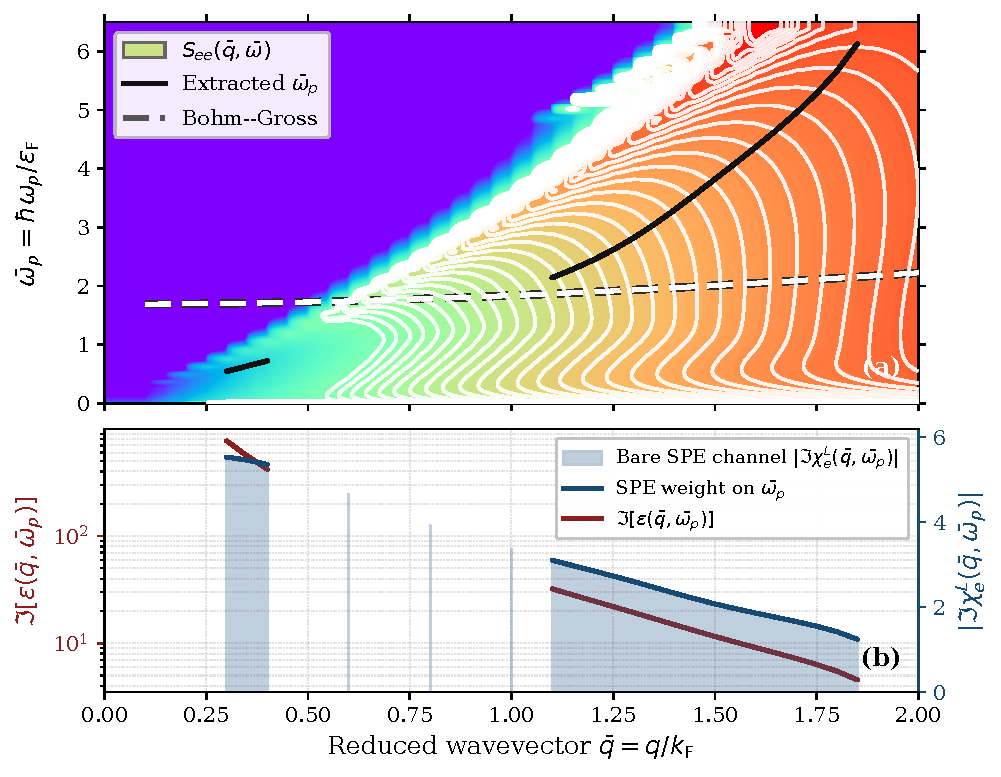
\includegraphics[width=\textwidth]{../output/plasmon_dispersion.pdf}
\vfill
\registerstandalonefigurelabel{fig:plasmon-dispersion}
\figurepaneltag{Fig.~\thesubmitfig}
\end{figure}

\panelpagefigure[fig:t0-limit-validation]{../output/t0_analytic_re_contour.pdf}{fig:t0-re-2d}
\panelpagefigure{../output/t0_analytic_im_contour.pdf}{fig:t0-im-2d}
\panelpagefigure{../output/t0_limit_validation.pdf}{fig:t0-1d-slice}

\panelpagefigure[fig:thermal-anatomy]{../output/thermal_anatomy_a.pdf}{fig:thermal-anatomy-a}
\panelpagefigure{../output/thermal_anatomy_b.pdf}{fig:thermal-anatomy-b}
\panelpagefigure{../output/thermal_anatomy_c.pdf}{fig:thermal-anatomy-c}
\panelpagefigure{../output/thermal_anatomy_d.pdf}{fig:thermal-anatomy-d}

\panelpagefigure[fig:Sq-gamma]{../output/Sq_gamma_ee.pdf}{fig:Sq-gamma-ee}
\panelpagefigure{../output/Sq_gamma_ii.pdf}{fig:Sq-gamma-ii}
\panelpagefigure{../output/Sq_gamma_ei.pdf}{fig:Sq-gamma-ei}

\end{document}
